\section{Experiments}
\label{sec:eval}
In this section, we conduct experiments on four classifiers, various sampling
strategies on eight different many-class short text datasets. 
Our experiments are conducted from four aspects:
\begin{enumerate*}[label=(\arabic*)] 
	\item we show that fastText is a better classifier for AL 
compared with CNN, LSTM as well as BERT. 
	\item we illustrate the significance of AL in alleviating the 
labeling burden especially for many-class. 
	\item we compare the performance of different AL sampling strategies on different classifiers and show the advantage of frequency tuning. 
	\item we try to find out the correlation between different characteristics of datasets with AL performance.
\end{enumerate*}

\begin{figure*}[th]
	\centering
	%\subfloat[Complaint]{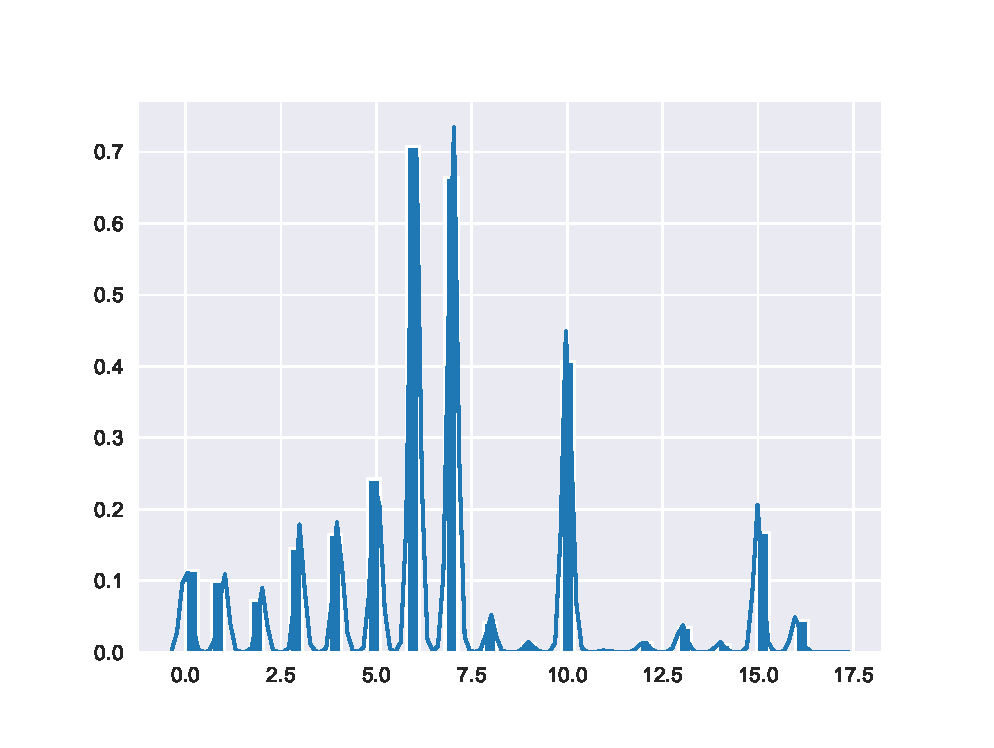
\includegraphics[width=0.2\textwidth]{figs/complaint.eps}}
    \begin{center}
	\subfloat[Reuters (RT)]{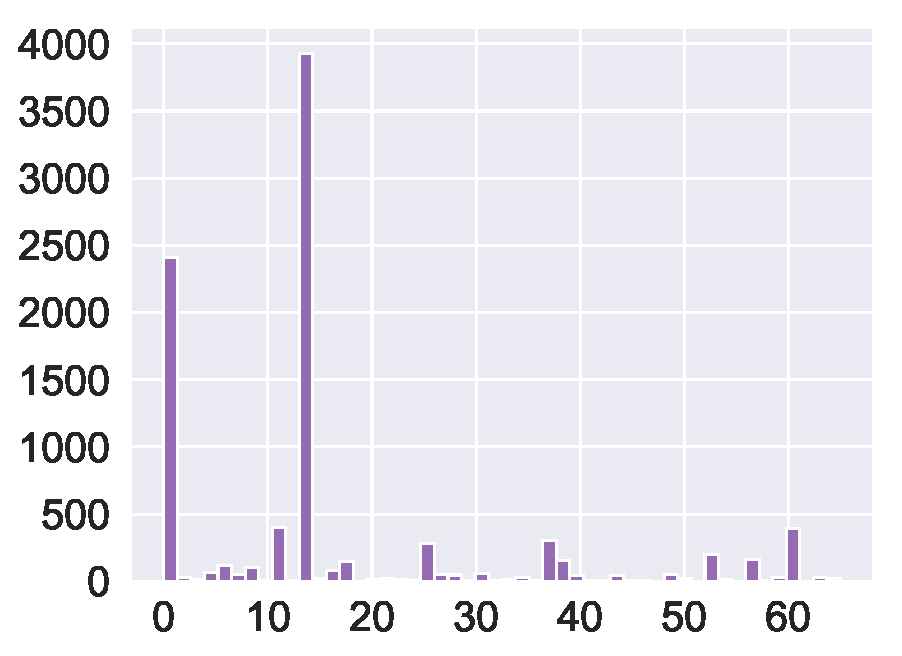
\includegraphics[width=0.2\textwidth, height=0.11\textheight]{figs/reuters_dis.eps}}
	\subfloat[HuffPost (HP)]{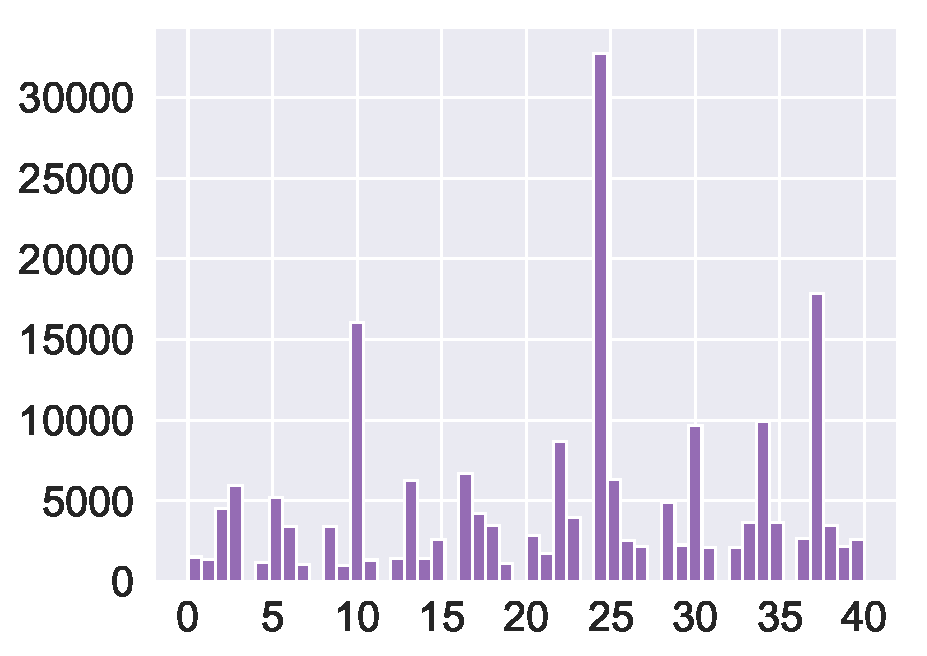
\includegraphics[width=0.2\textwidth, height=0.11\textheight]{figs/news_dis.eps}}
	\subfloat[Biomedical (Bio)]{\includegraphics[width=0.2\textwidth, height=0.11\textheight]{figs/bio_dis.eps}}
	\subfloat[Search Snippets (SS)]{\includegraphics[width=0.2\textwidth, height=0.11\textheight]{figs/search_dis.eps}}\newline      
    \end{center}

	\subfloat[Emoji (EM)]{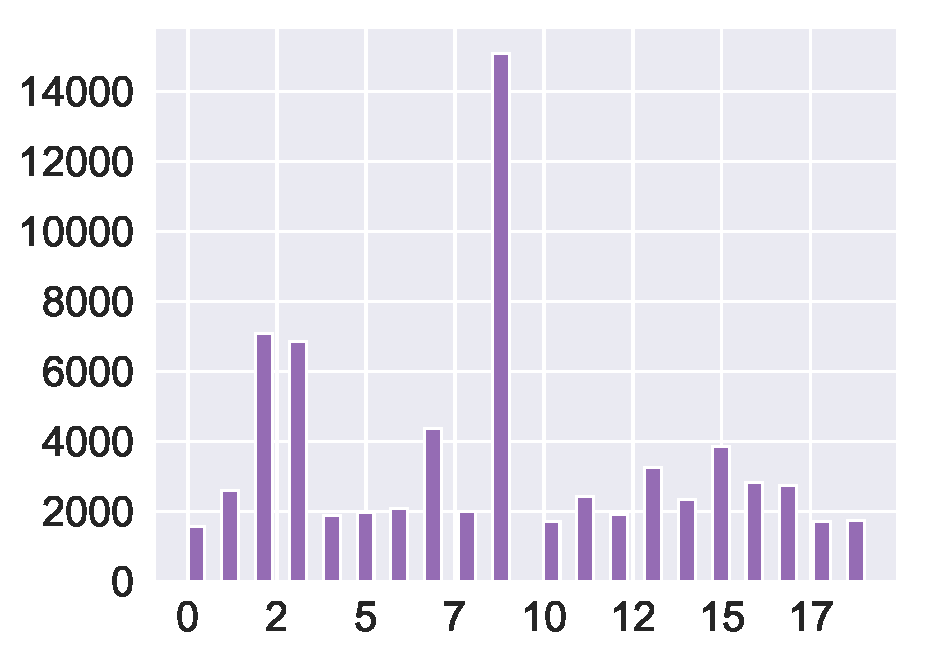
\includegraphics[width=0.2\textwidth, height=0.11\textheight]{figs/emoji_dis.eps}}
	\subfloat[TNEWS (TN)]{\includegraphics[width=0.2\textwidth, height=0.11\textheight]{figs/tnews_dis.eps}}
	\subfloat[GCS]{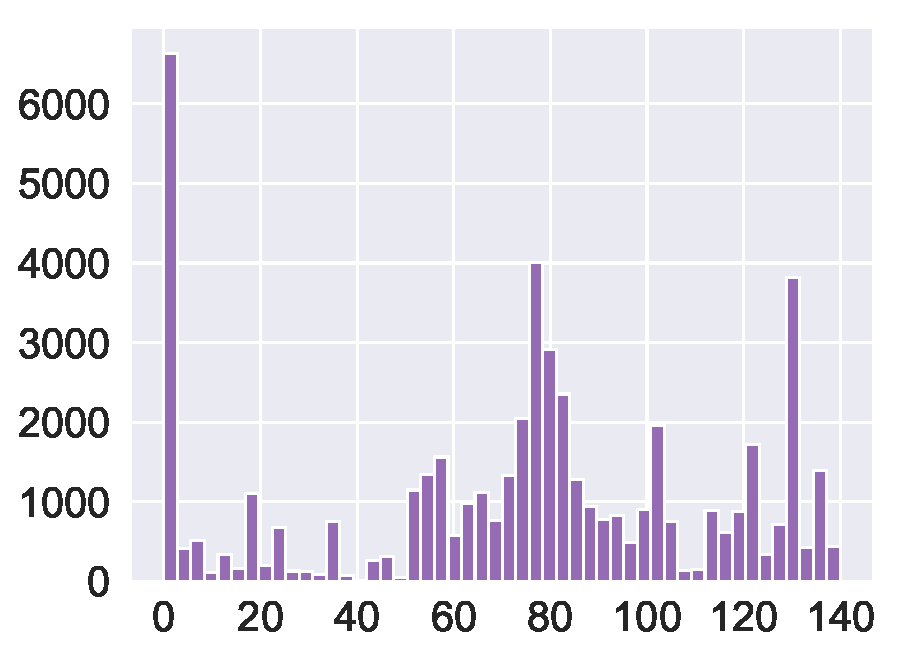
\includegraphics[width=0.2\textwidth, height=0.11\textheight]{figs/yanjing_dis.eps}}
	\subfloat[Book (BK)]{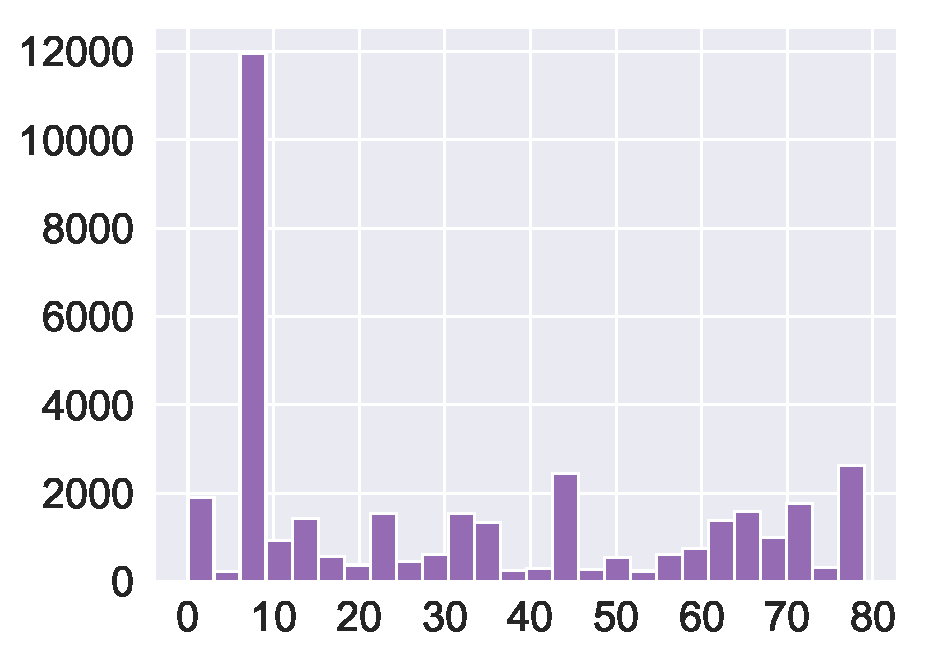
\includegraphics[width=0.2\textwidth, height=0.11\textheight]{figs/book_dis.eps}}\newline
	
	\caption{Label Distribution of Datasets (with abbreviations) (Classes (X) vs. Number of 
instances (Y)). 
%\KZ{The y axis should be the number instances for a class. Why is it less than 1}
} 
\label{fig:distribution}
\end{figure*}

\begin{table*}[th]
	\small
	\centering
	\begin{threeparttable}
	\begin{tabular}{ccccccccc}
		\toprule
		& Reuters\tnote{1}  & HuffPost\tnote{2} & Biomedical\tnote{3}  & SearchSnippets\tnote{3} & Emoji\tnote{4}  & TNEWS \tnote{5}   & GCS\tnote{6}  & Book\tnote{7} \\ \hline
		Classes       & 66      & 41    &20&8  & 20 & 15         & 141                & 80    \\
		\#Samples     & 9,442   &200,853   &20,000&12,340    &70,000       & 325,285    & 63,792                &36,816      \\
		Language      & Eng      & Eng                  & Eng          & Eng    &Eng& Ch         & Ch   &Ch    \\
		Avg Tokens/sample & 6.2      &10.7    &12.9&17.9   &14.5    & 13.2        &     6.0      &6.2      \\
		Min Tokens/sample & 1 &1 & 1 & 1 &1&1         &1&1\\
		Max Tokens/sample & 21 &59 &53&48 &89 & 90 & 151    &170 \\
		OOV &1,020&7,018&4,183&8,156 &34,012 &97,154&4,939   &4,468\\
		Vocabulary& 7,715&55,442&18,787&29,154&82,742&144,235&10,591     &9,722\\
		Desc.         & news title  & news title &paper title&web search transaction &tweets &news title& customer  &customer
   \\ 
	& & &  & & &&request sentence &request sentence \\
		Label         & topic     & topic    &topic &domain  &emoji   & topic   & intention                      &intention\\
		\bottomrule              
	\end{tabular}

\begin{tablenotes}
	\item[1] \url{https://archive.ics.uci.edu/ml/datasets/reuters-21578+text+categorization+collection}
	\item[2] \url{https://www.kaggle.com/rmisra/news-category-dataset}
	\item[3] \url{https://github.com/jacoxu/STC2}
	\item[4] \url{https://www.kaggle.com/hariharasudhanas/twitter-emoji-prediction}
	\item[5] \url{https://github.com/ChineseGLUE/ChineseGLUE}
	\item[6] \url{http://Anonimized.for.blind.review}
	\item[7] \url{http://Anonimized.for.blind.review}
	%\item[7] \url{https://competitions.codalab.org/competitions/17344}
	
\end{tablenotes}

\end{threeparttable}
\caption{Statistics of Datasets.}

\label{table:statsOfDataset}
\end{table*}
\begin{table*}[th]
	\small
	\centering
	\begin{tabular}{c P{11cm}P{3cm}}
	\hline
	Dataset & Input     &      Output          \\ \hline
	Reuters     & COLOMBIA OPENS APRIL/MAY COFFEE REGISTRATIONS & coffee         \\ 
	HuffPost &South Korean President Meets North Korea's Kim Jong Un To Talk Trump Summit &WORLD NEWS\\ 
	Biomediocal & effects of perceptual training at three age levels & aging \\ 
	SearchSnippets & schneier blog archives bank sued for schneier security bank sued unauthorized transaction bank america sued unauthorized transaction mistake & business\\ 
	Emoji & this summer was one to remember because of them @ North Cypress& \_red\_heart\_ \\
	TNEWS & \begin{CJK}{UTF8}{gbsn}理想的游戏手机应该是怎样的?(What should an ideal gaming phone look like?)\end{CJK} & news\_tech \\ 
	GCS     & \begin{CJK}{UTF8}{gbsn}货发了没?(Have you shipped my stuff?)\end{CJK} &  current shipping status      \\ 
	Book & \begin{CJK}{UTF8}{gbsn}退货怎么走流程?(
		How to return the goods)\end{CJK}	&  after-sales operation \\ \hline
	
	\end{tabular}
	\caption{Examples of Dataset.}
	\label{table:exampleOfDataset}
	\end{table*}

\subsection{Experimental Setup}
\subsubsection{Datasets} 

The statistics of the datasets are summarized in \tabref{table:statsOfDataset}
and \figref{fig:distribution}.
%Consumer Complaint Database \footnote{https://catalog.data.gov/dataset/consumer-complaint-database}, 
%Glasses Custom Service (GSC) Dataset.  TNEWS dataset is provided by ByteDance 
%and GCS is offered by Leyan Tech. 
In order to give a rough understanding of datasets, we show one example of
each dataset in \tabref{table:exampleOfDataset}. 
Moreover, in order to understand the difference between many-class tasks and few-class ones, 
we further generate sub-datasets with varying number of classes. 
For each dataset, we rank the classes by the size and select top $k$ classes and forms 
a subset dataset with instances of those $k$ classes.
In our experiment, we set $k$ to 2, 5 and 10. Thus, each dataset has four variants,
including the original dataset itself.

%The detailed information is included in table \ref{table:statsOfDataset}. 
% Moreover, in order to understand the difference between many-class tasks and few-class ones, 
% we further generate sub-datasets with varying number of classes. 
% We rank the classes by the size for each dataset and select top $k$ classes and forms 
% a subset dataset with instances of those $k$ classes. 
% In our experiment, we set $k$ to 2, 5, 10, respectively. Thus, each dataset has four variants,
% including the original dataset itself.
% The first three datasets are in English while the last two are in Chinese. 
% Table ~\ref{table:detailsOfDataset} shows the input and output field of each dataset along with number classes.

% Table ~\ref{table:detailsOfDataset} shows the input and output field of each dataset. An example of Complaint Dataset and Glasses Custom Service Dataset displays in Table ~\ref{table:exampleOfDataset}. 

% \begin{table}[]
% 	\begin{tabular}{ccc}
% 		\hline
% 		& Input     & Output              \\ \hline
% 		Complaint     & complaint & product+subproduct          \\
% 		Reuters       & title     & topics                      \\
% 		SO & post      & tags                       \\
% 		TNEWS         & title     & category                   \\
% 		GCS       &    customer request sentence      &       intention                    \\ \hline
% 	\end{tabular}
% \caption{Input and Output of Dataset. SO is StackOverflow. GCS is Glasses Custom Service.}
% \label{table:detailsOfDataset}
% \end{table}

% \multicolomn{1}{c}{Output}

\subsubsection{Preprocessing}
We use NLTK\footnote{https://github.com/nltk/nltk} for English and jieba\footnote{https://github.com/fxsjy/jieba} for Chinese text.
We remove the stopwords and filter out bad symbols. 
We use 300-dimensional GloVe word embeddings \cite{pennington2014glove} 
for English and fastText wiki-news embeddings \cite{mikolov2018advances} for Chinese.
% Specially, we choose a word2vec embedding trained on StackOverflow posts\footnote{https://github.com/vefstathiou/SO\_word2vec}  to solve OOV (Out-of-Vocabulary) on SQD and StackOverflow. We randomly split each subset into 80\% training and 20\% test. 

\subsubsection{Model and Hyperparameters}
We use the most vanilla configuration for LSTM and CNN. We use single-layer unidirectional LSTM whose hidden state dimension is 256. The hidden state of last LSTM cell is considered the feature vector. For CNN, we follow the model architecture of \cite{kim2014convolutional}. The filter window sizes are 2, 3, 4 with 200 feature maps each. We consider the vector after max-pooling step as feature vector. For the above two models, the feature vector is passed through a single fully-connected layer to calculate the probability distribution. 

For fastText, we specify the API parameters as follows: \emph{wordNgrams=2, minn=2, maxn=3}. 

We choose \emph{BERT-Base, Uncased} for English and \emph{BERT-Base, Chinese} for Chinese.

The training epoch is 5 for BERT and 25 for other three models.


\subsubsection{AL Parameters and Evaluation Metric}
% To compare the performance of sampling strategies on different number of classes, we further create smaller subsets from the datasets with 2, 5, 10 and all classes according to the number of samples of the classes. 

In order to achieve comparable results, we set the batch size $\mathcal{B}$ to 100, namely, selecting 100 points at one time step. For each subset, we typically start with 100 fixed data samples and stop at 3000 data samples. 
We select macro-average F1 score as our primary accuracy metric because it handles
class imbalance better than micro-F1. Finally, we record F1 score at each time step, 
and use the area under the curve (denoted as AUC*) as the evaluation criteria for different
sampling strategies. 

% We define strategies as follows: concatenation with \textit{freq} means the original method is tuned with $frequency$ and \textit{sqrtfreq} means tuning with $\sqrt{frequency}$. 
% We design three experiments \KZ{give the purposes of these 3 experiments}: 
% \begin{enumerate}[(a)]
% 	\item Comparison between our proposed method \textbf{Radius freq} and other traditionsampling strategies: \textbf{Random, Entropy, Density, Active, Center}.
% 	\item Comparison between vanilla method and tuned strategies: \textbf{Entropy, Entropy freq, Entropy sqrtfreq; Density, Density freq, Density sqrtfreq}.
% 	\item fastText using \textbf{Radius freq} sampling method, incrementally trained from 100 samples to all samples.
% \end{enumerate}

\subsection{Results and Analysis}
\label{sec:results}

\begin{figure*}[th!]%[!hbt]
\begin{center}
\subfloat[Legend]{\includegraphics[scale=0.55]{res/legend.eps}}
\end{center}
\noindent
	\begin{center}
		\subfloat[Reuters]{\includegraphics[width=0.23\textwidth]{res/ft_reuters_new_acc_all.eps}}
		\subfloat[HuffPost]{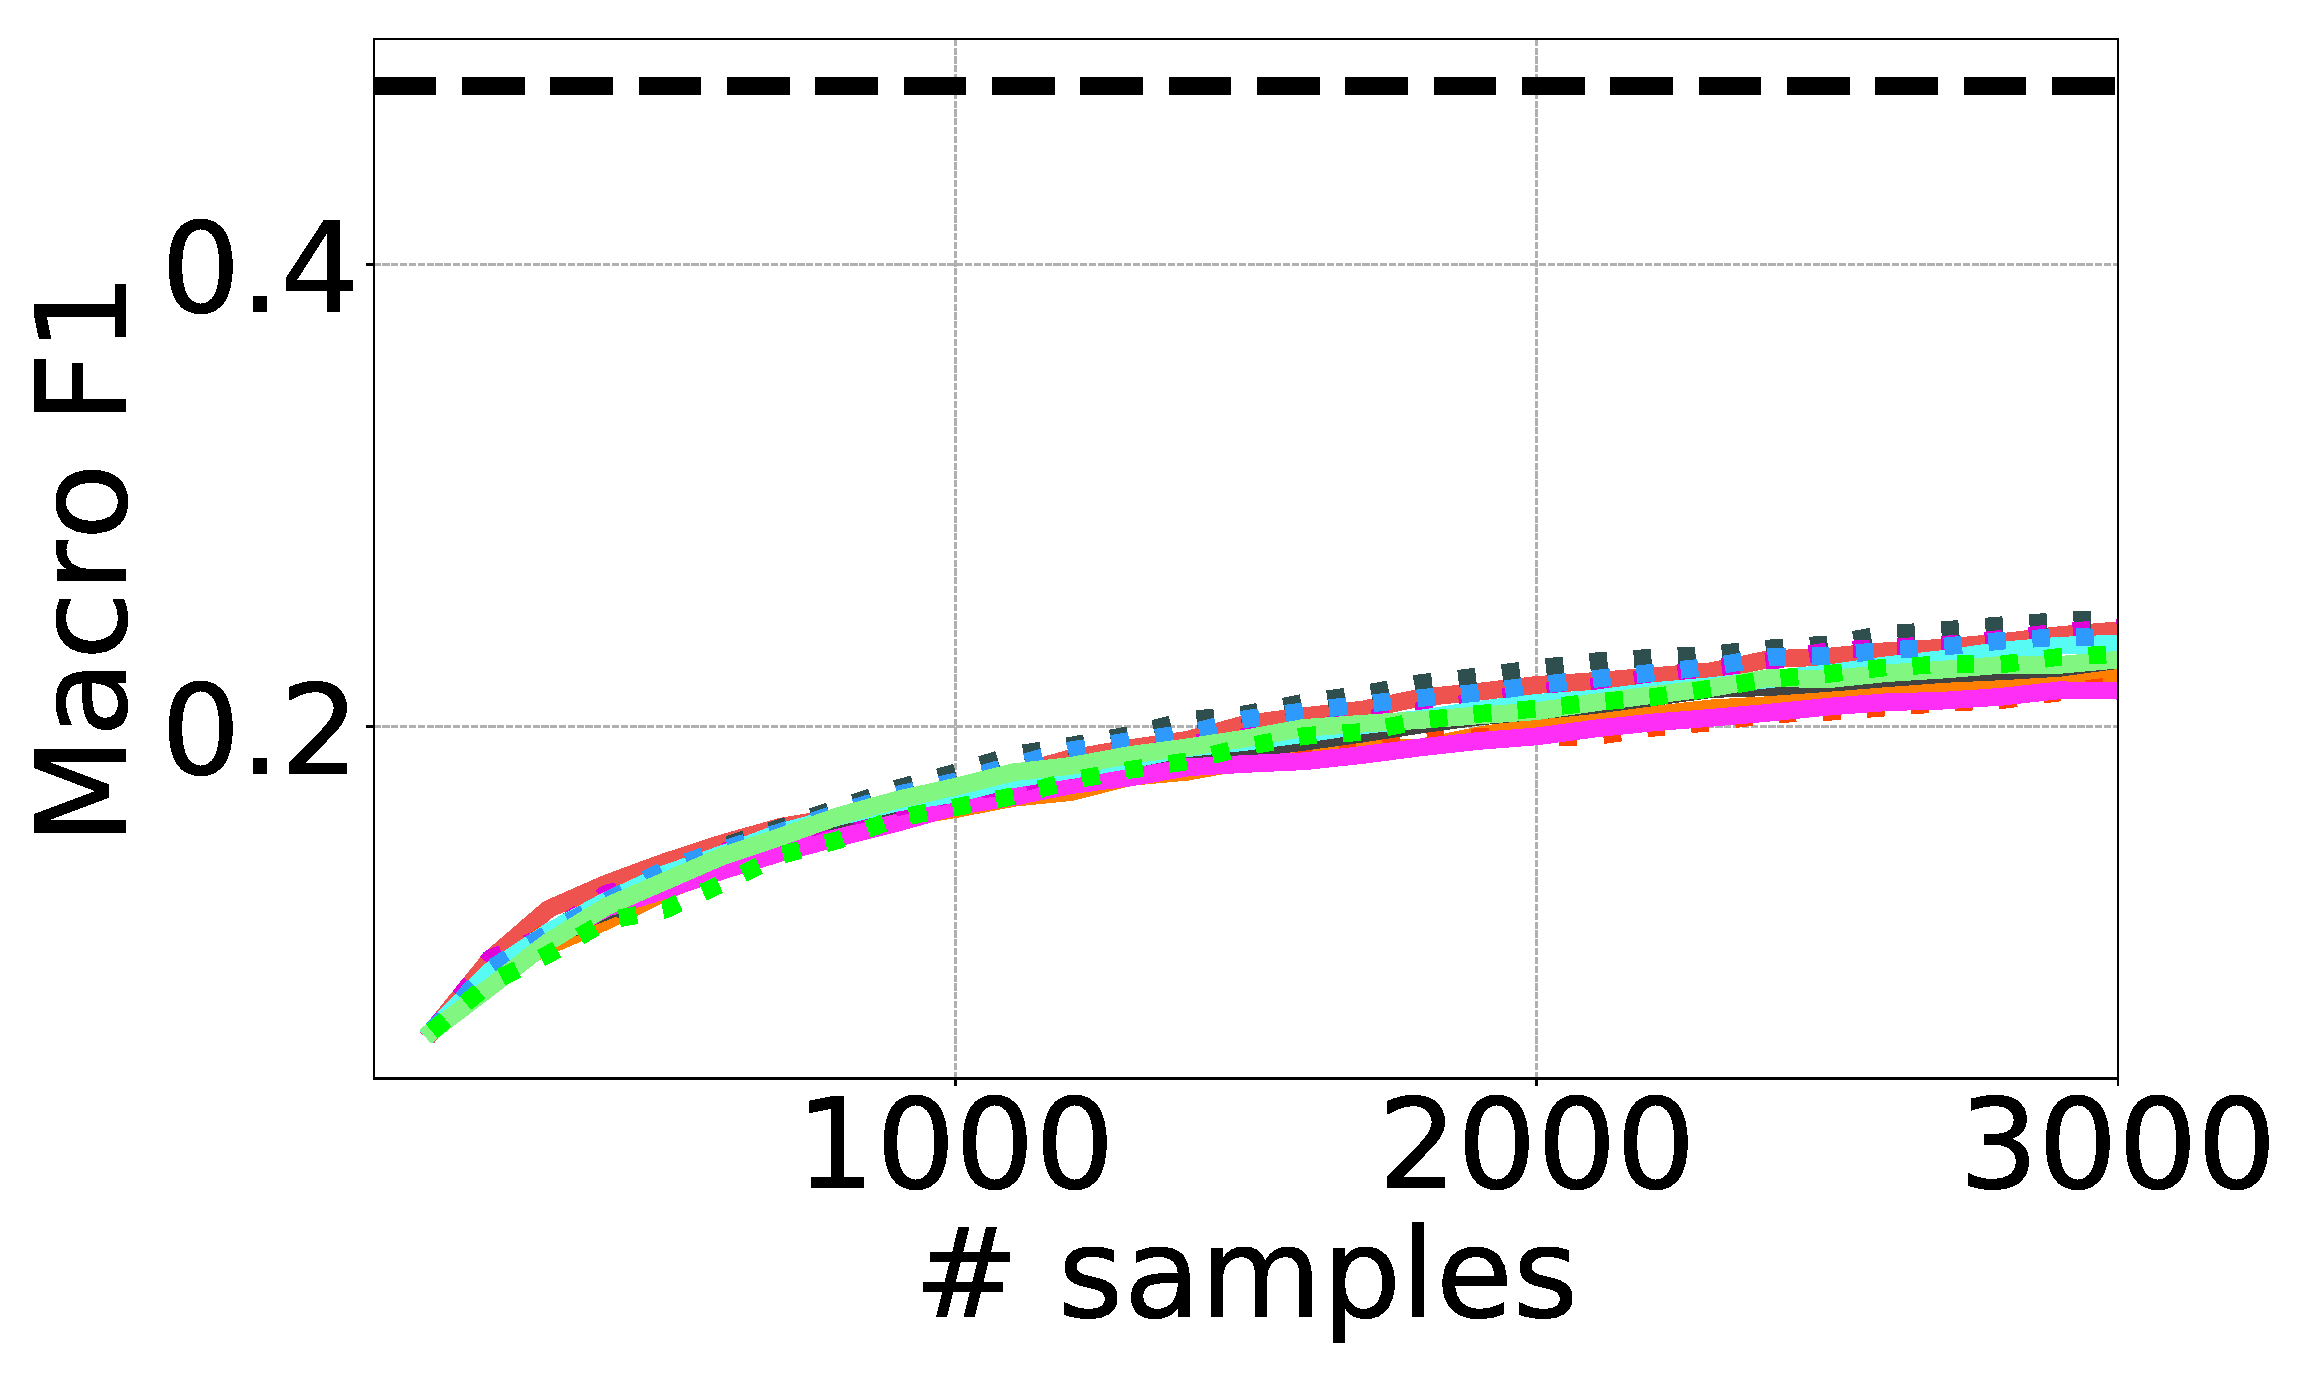
\includegraphics[width=0.23\textwidth]{res/ft_news_tokenized_norm_acc_all.eps}}
		\subfloat[Biomedical]{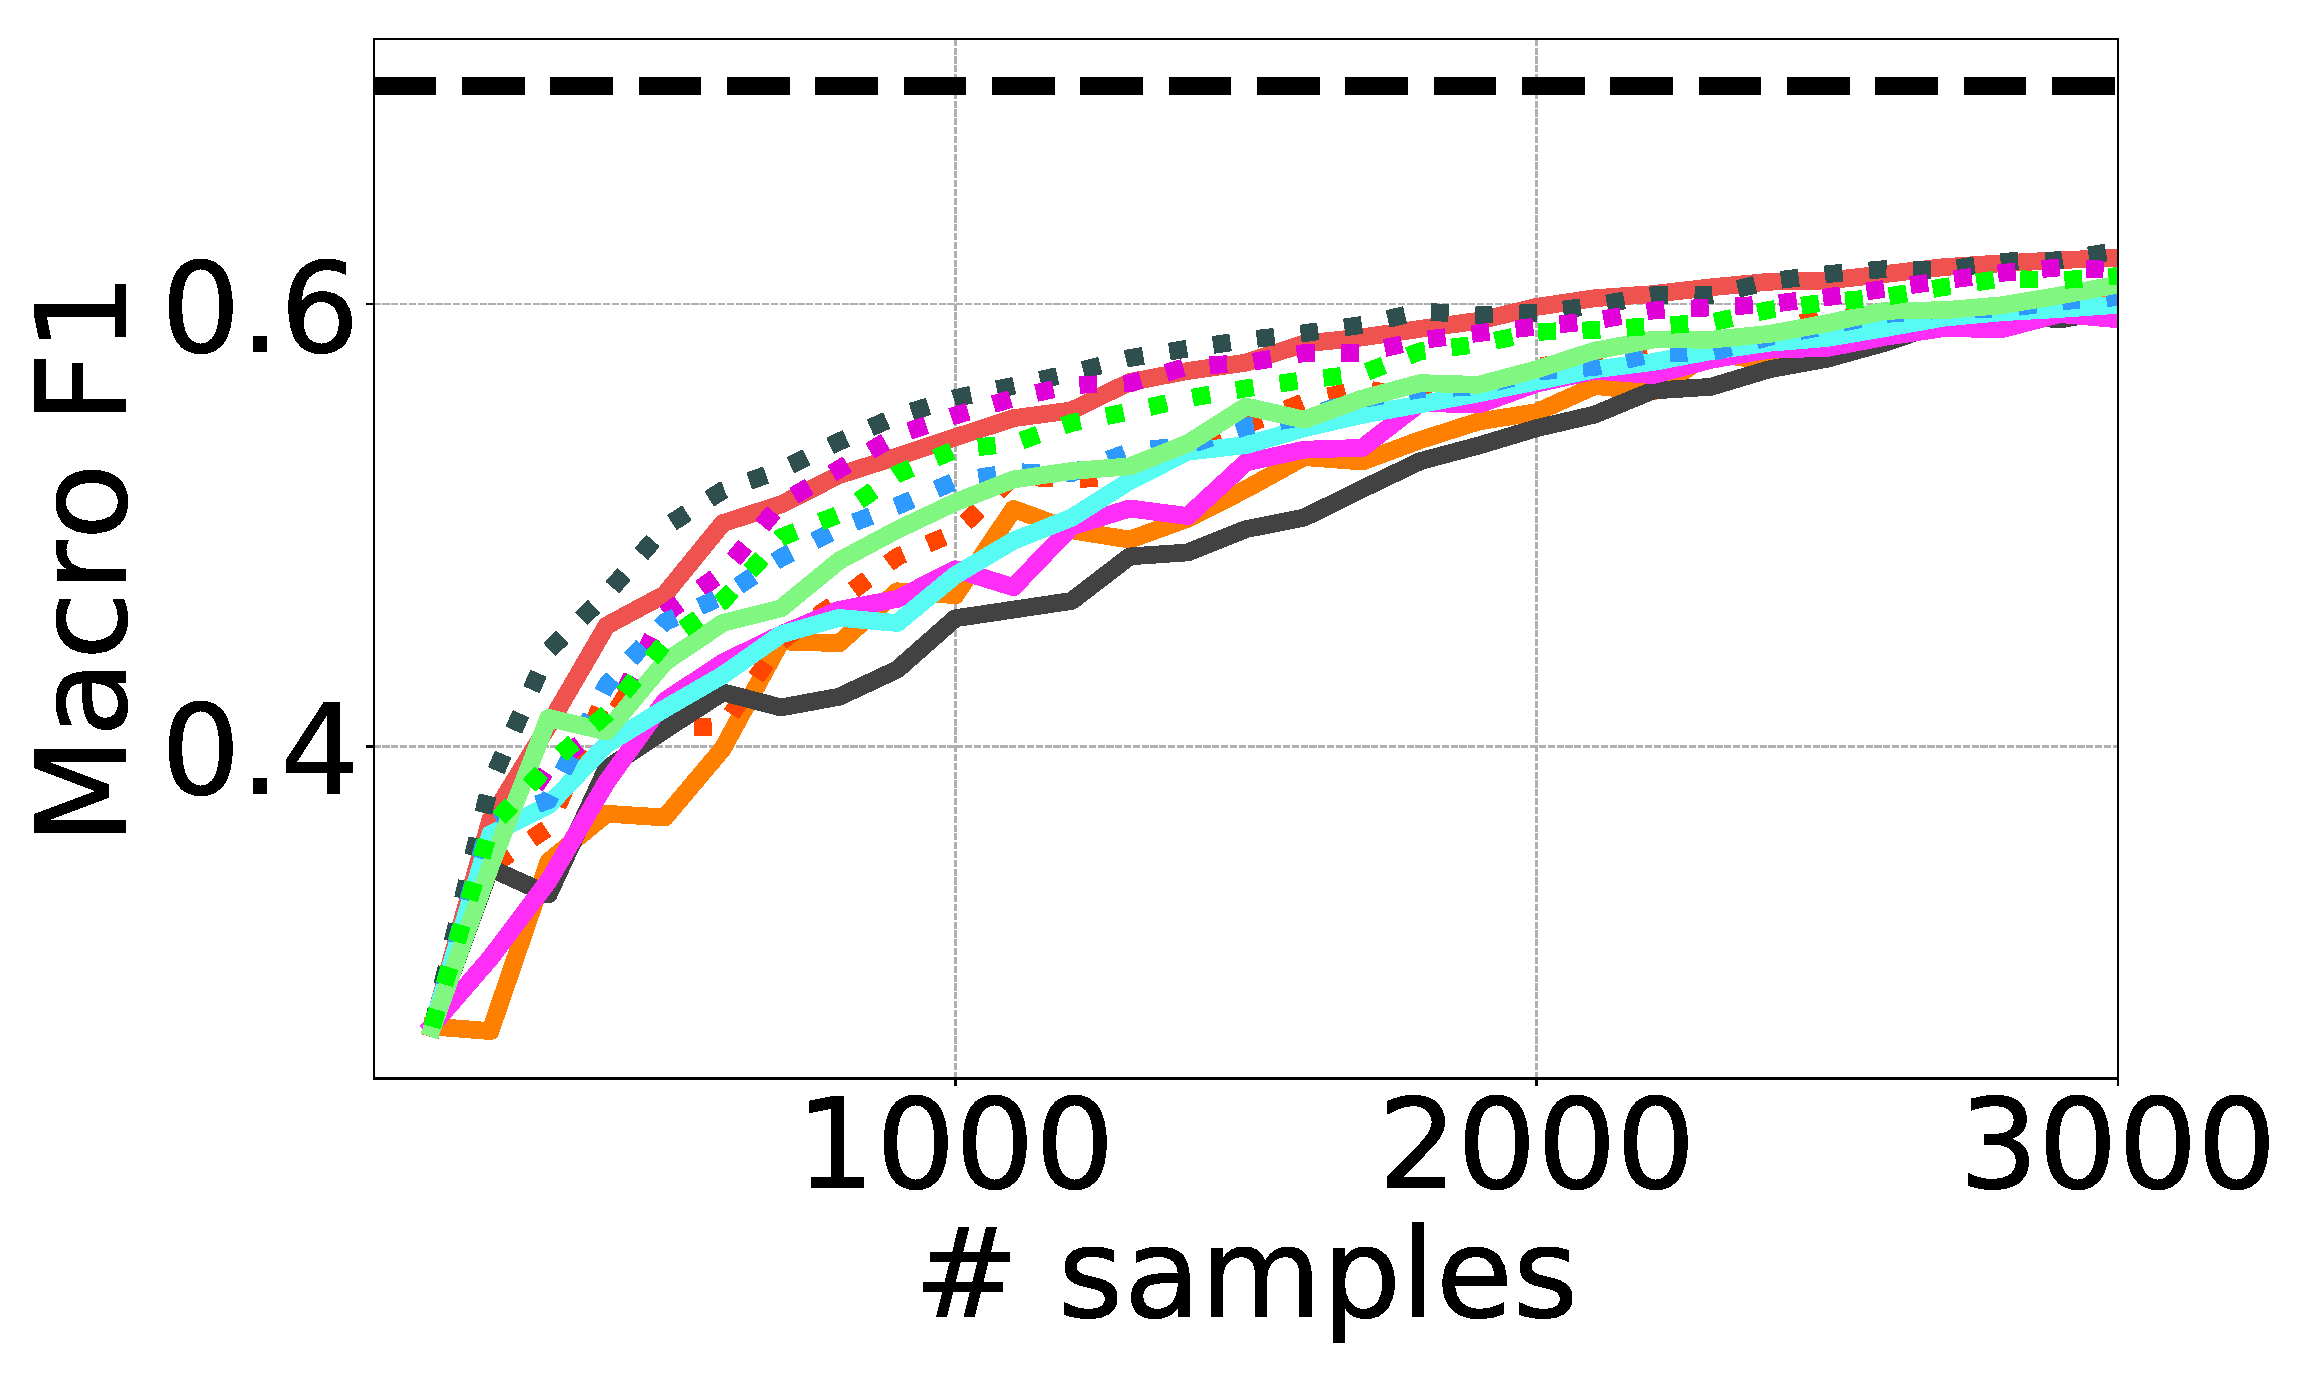
\includegraphics[width=0.23\textwidth]{res/ft_Biomedical_tokenized_acc_all.eps}} % \newline
		%\subfloat[StackOverflow]{\includegraphics[width=0.24\textwidth]{figs/ft_SO_tokenized_acc_all.pdf}}
		\subfloat[SearchSnippets]{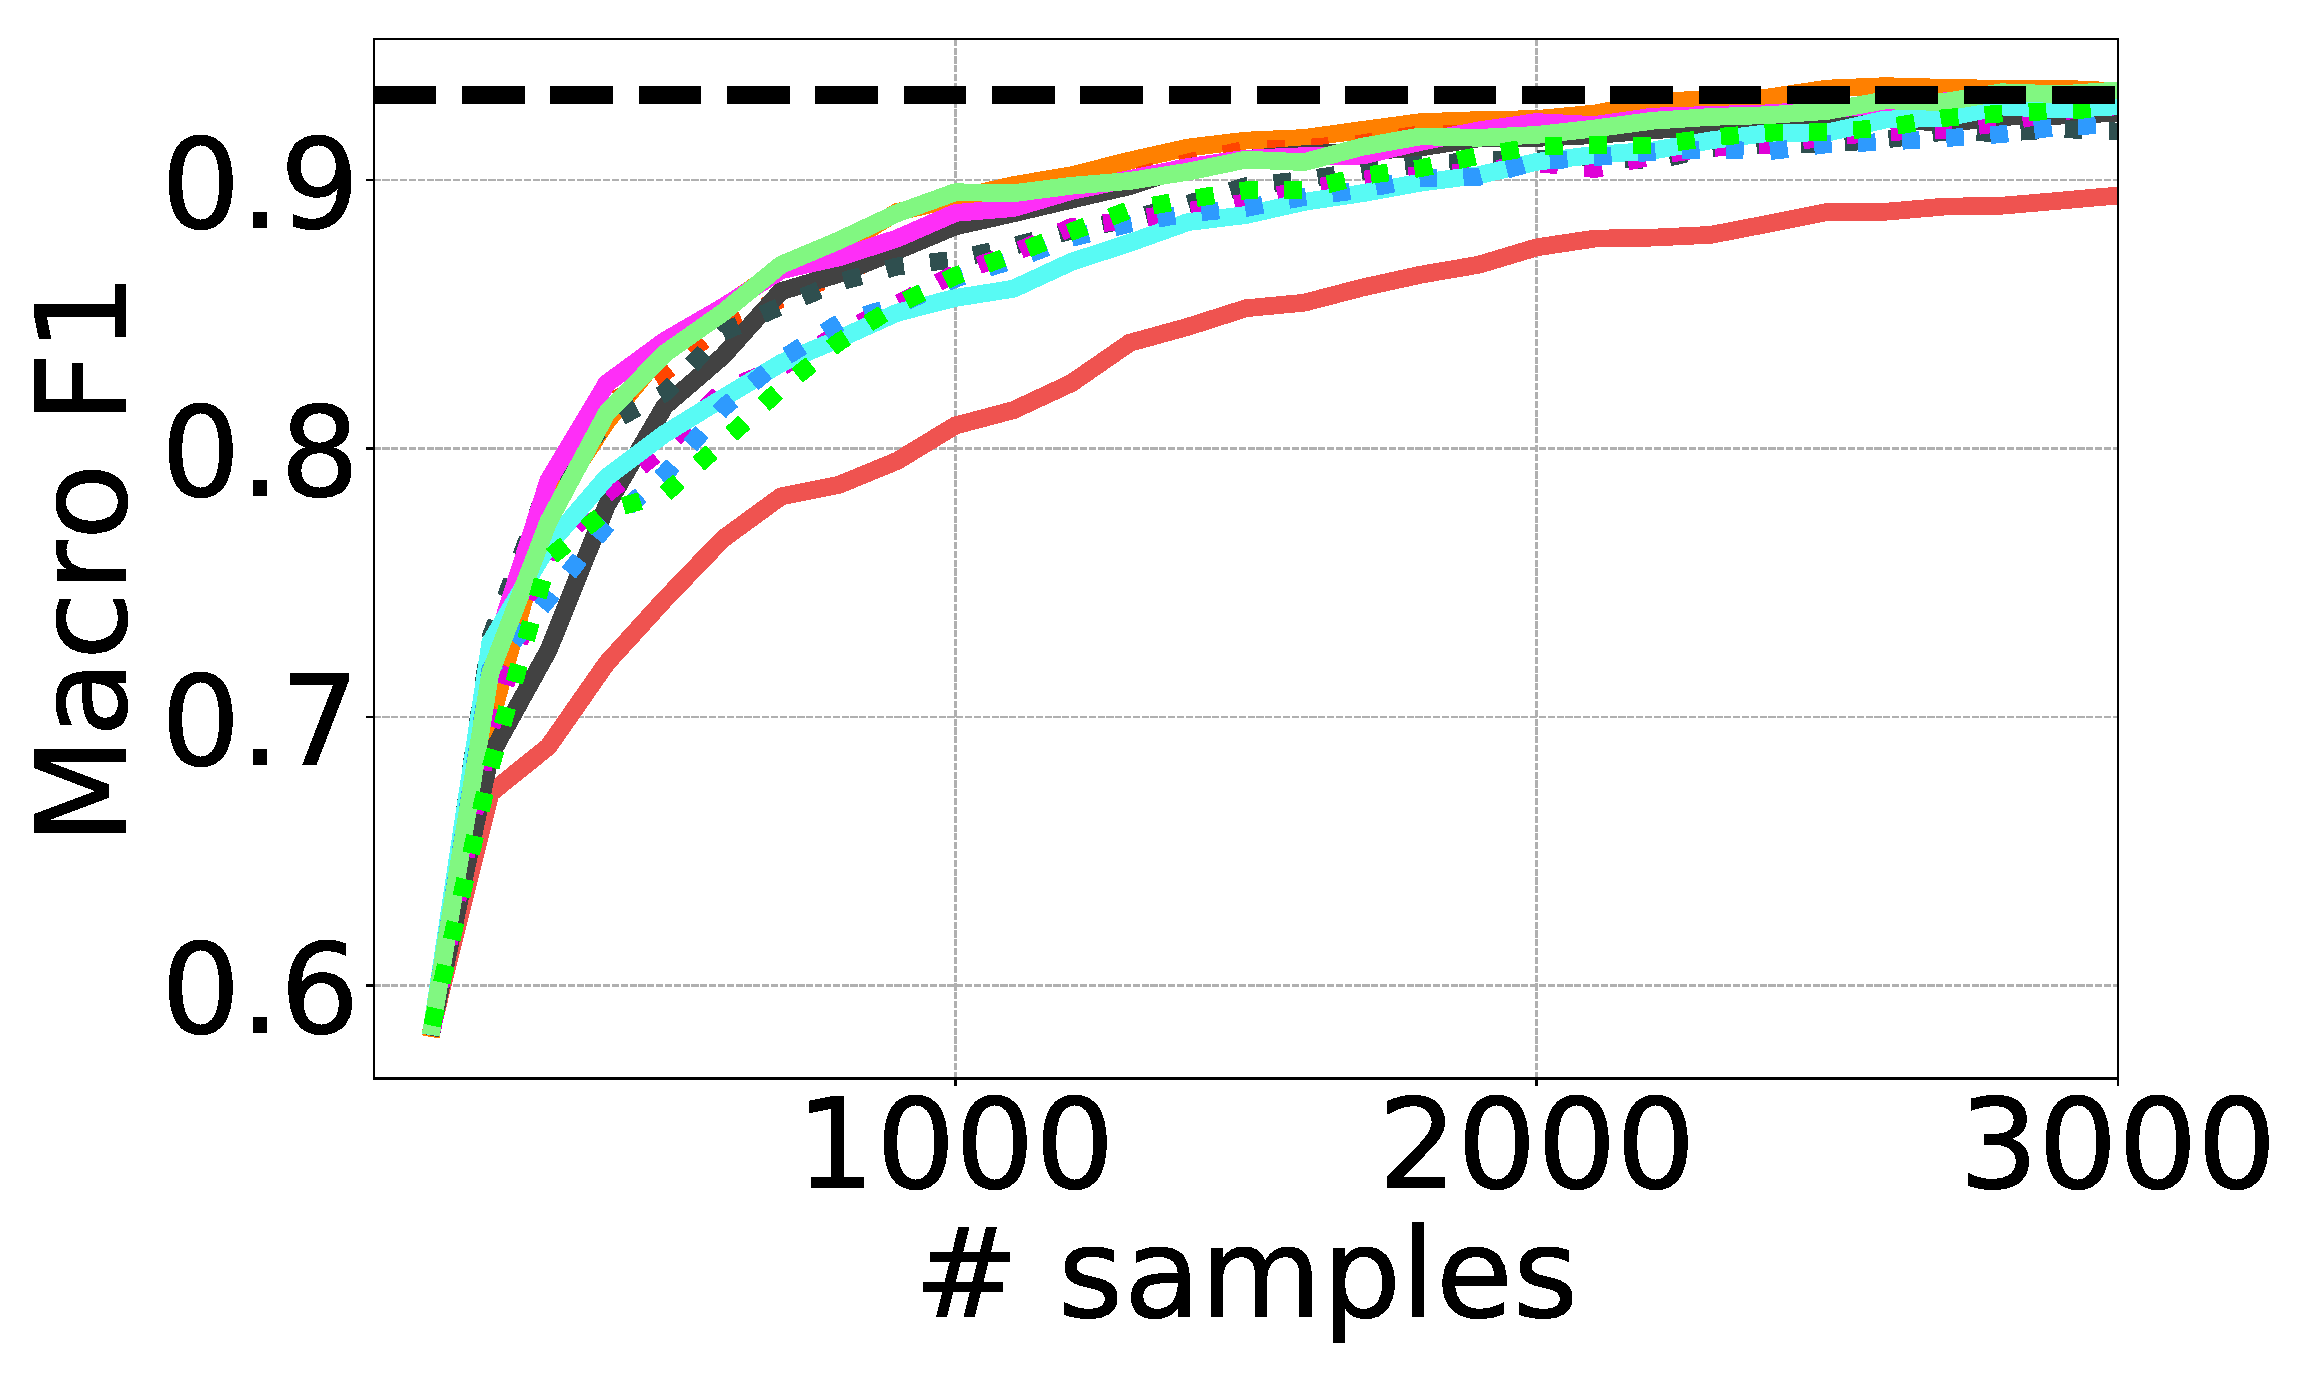
\includegraphics[width=0.23\textwidth]{res/ft_SearchSnippets_tokenized_acc_all.eps}}
	\end{center}
	\noindent
	
	\begin{center}
		\subfloat[Emoji]{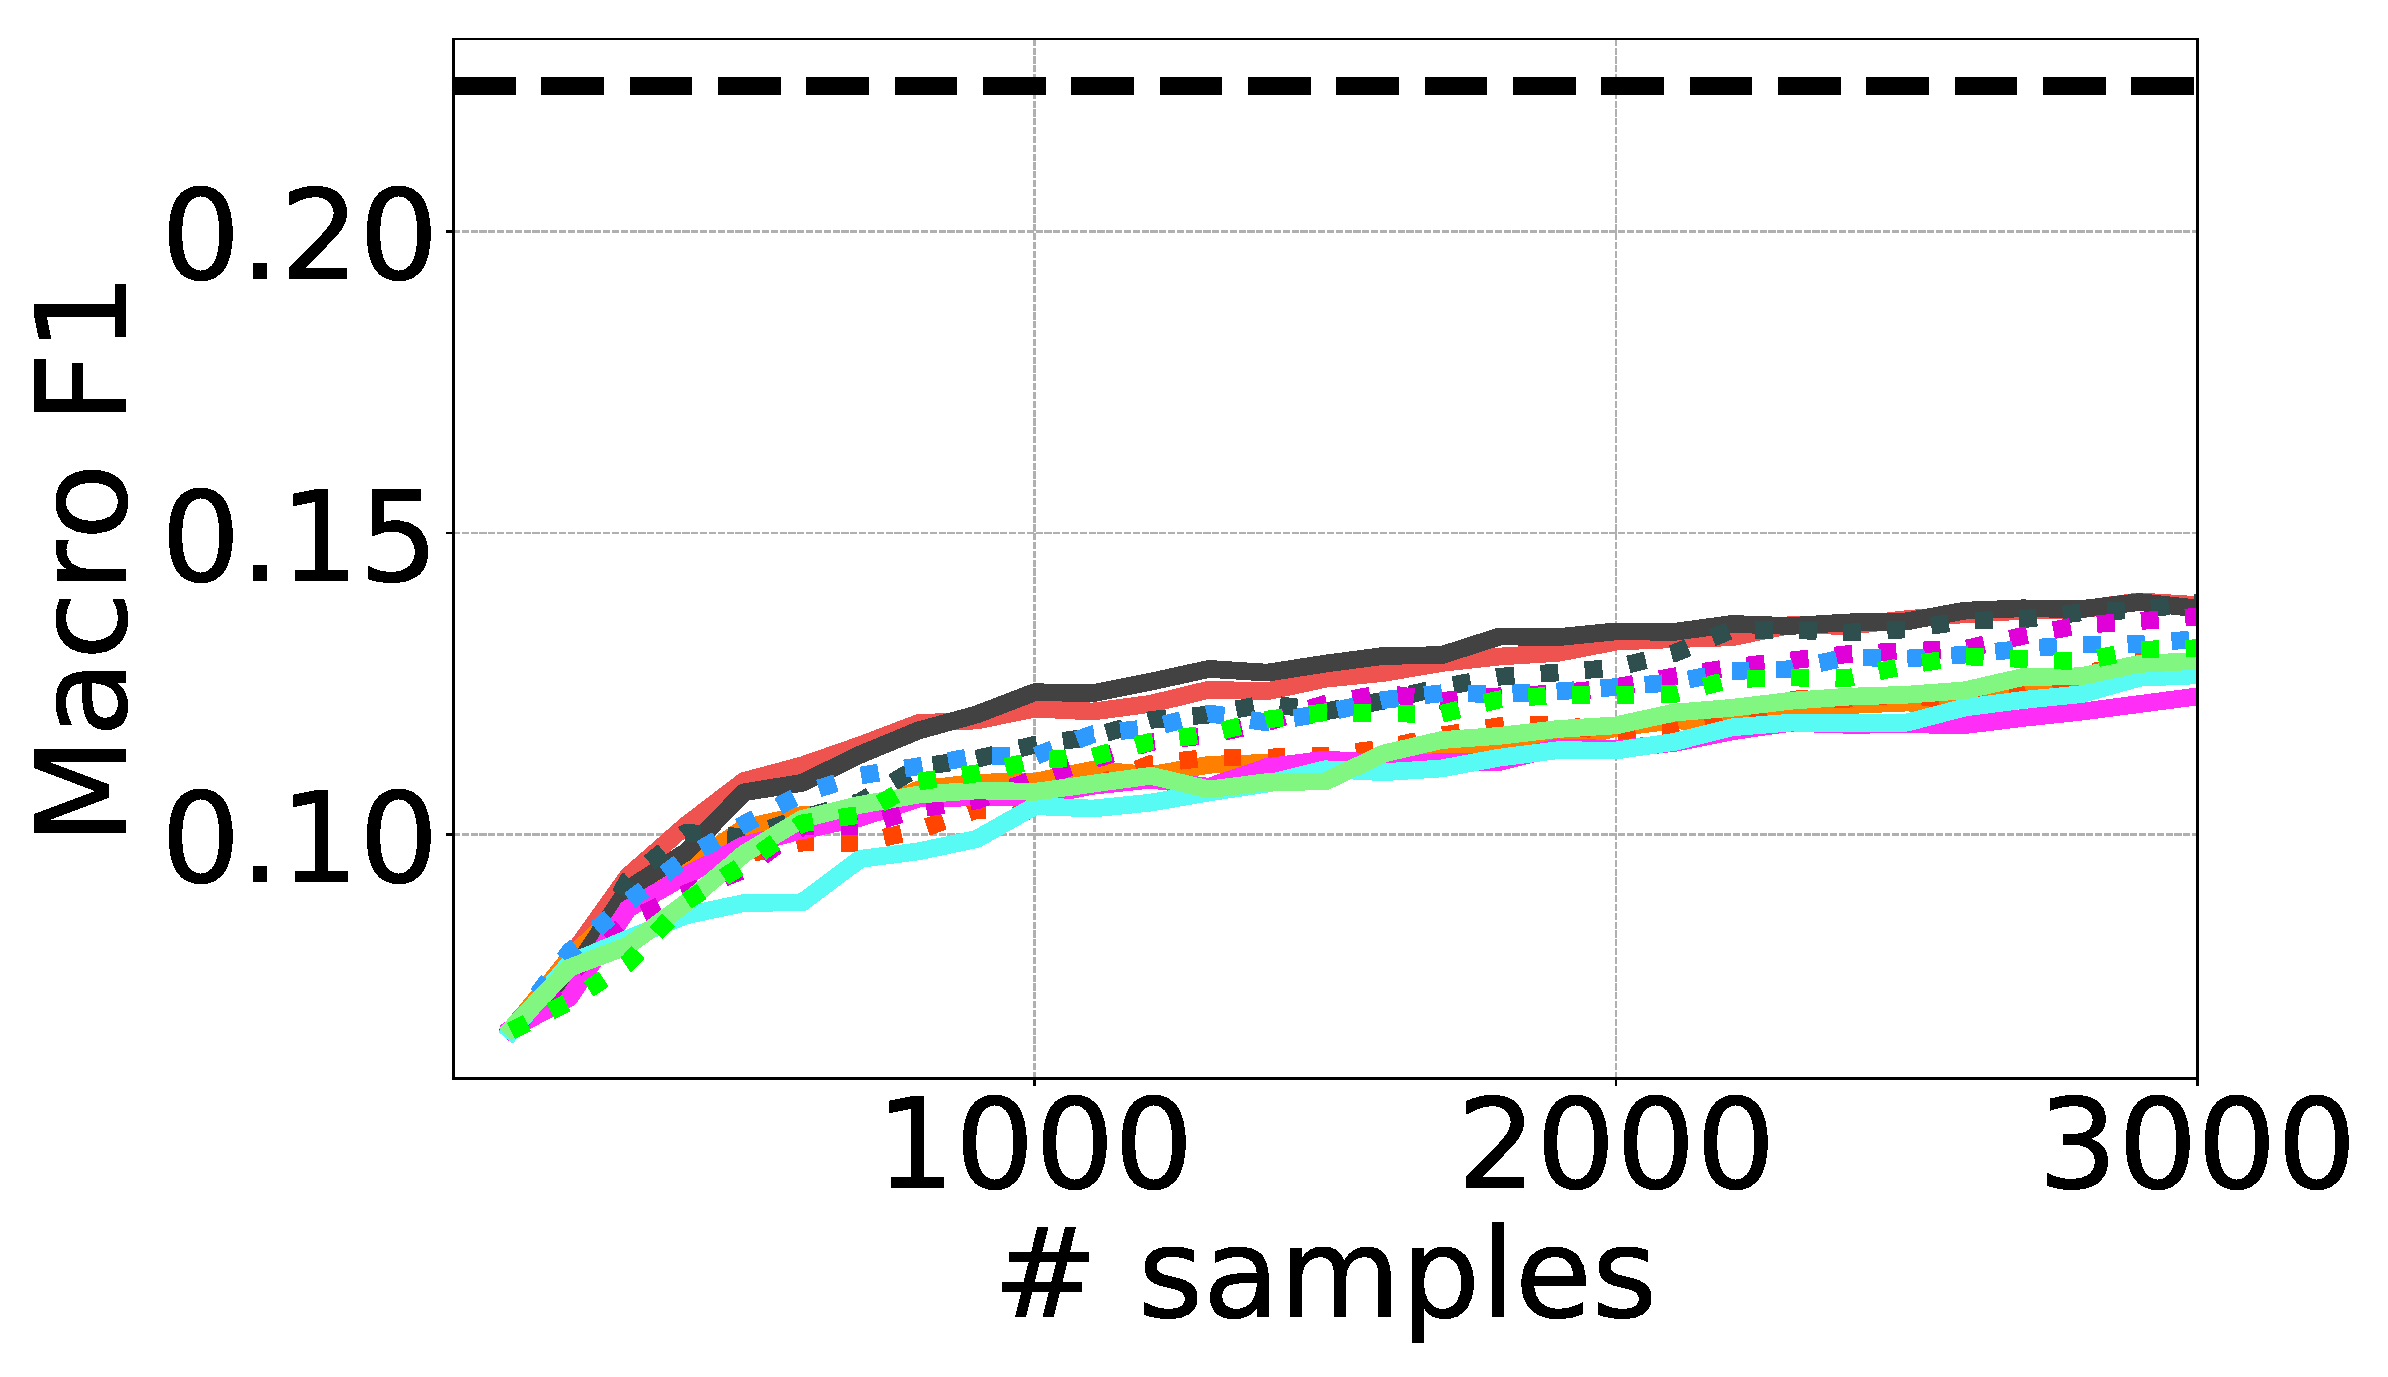
\includegraphics[width=0.23\textwidth]{res/ft_emoji_tokenized_acc_all.eps}}
		\subfloat[TNEWS]{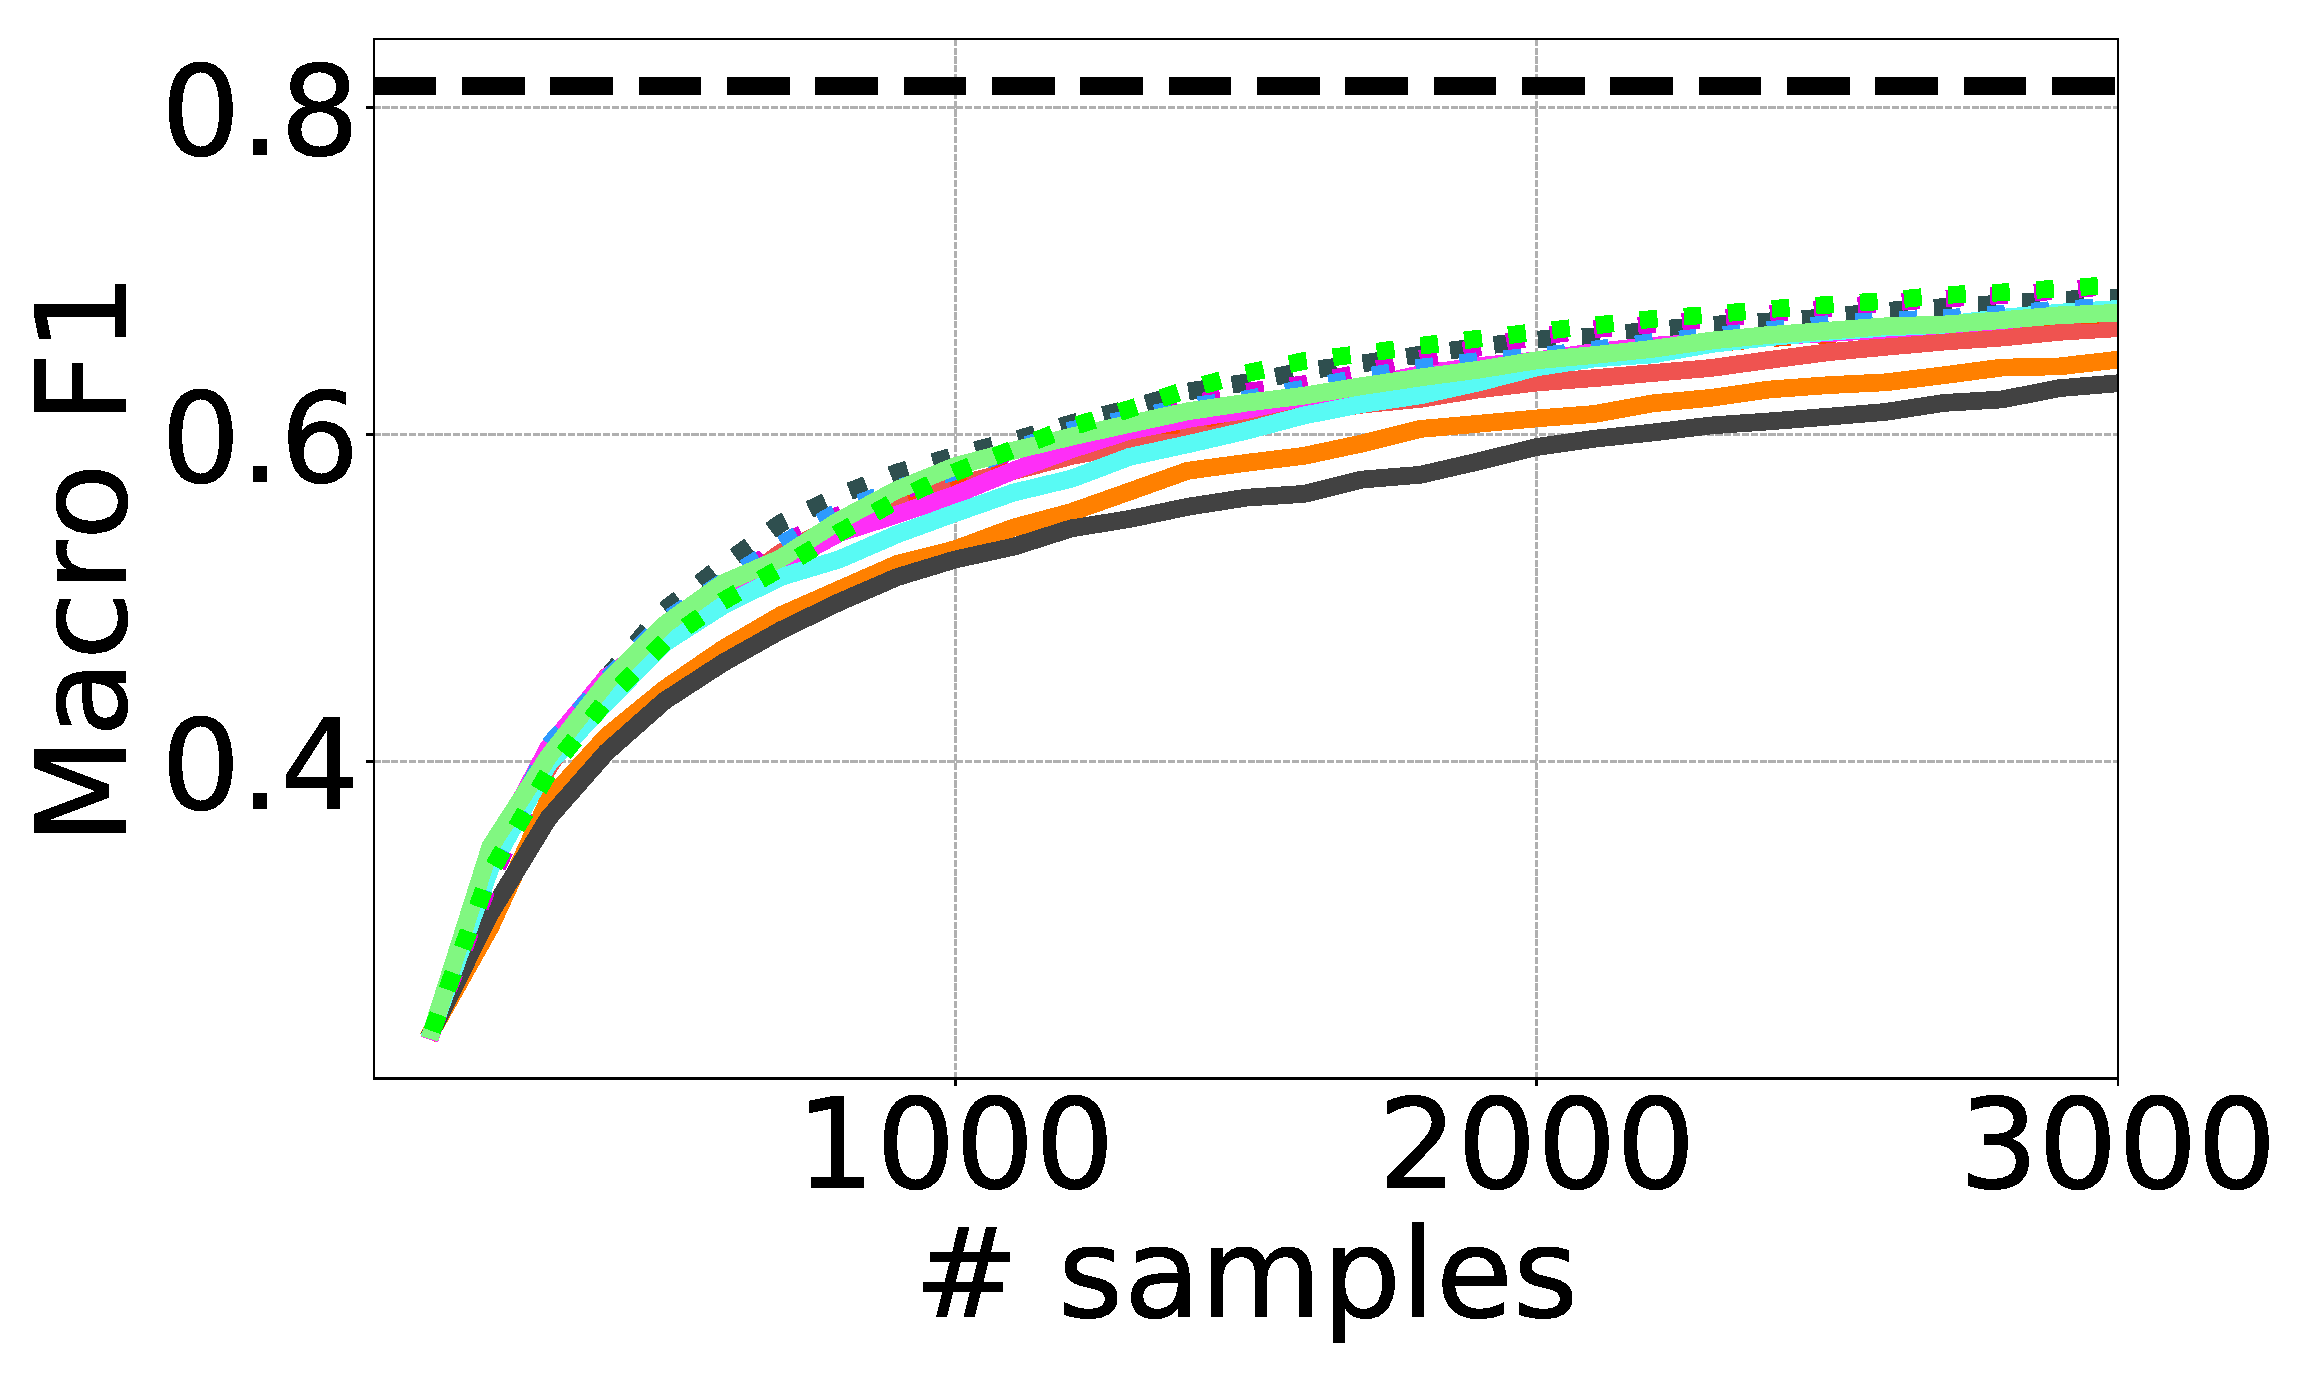
\includegraphics[width=0.23\textwidth]{res/ft_tnews_tokenized_acc_all.eps}} % \newline
		\subfloat[GCS]{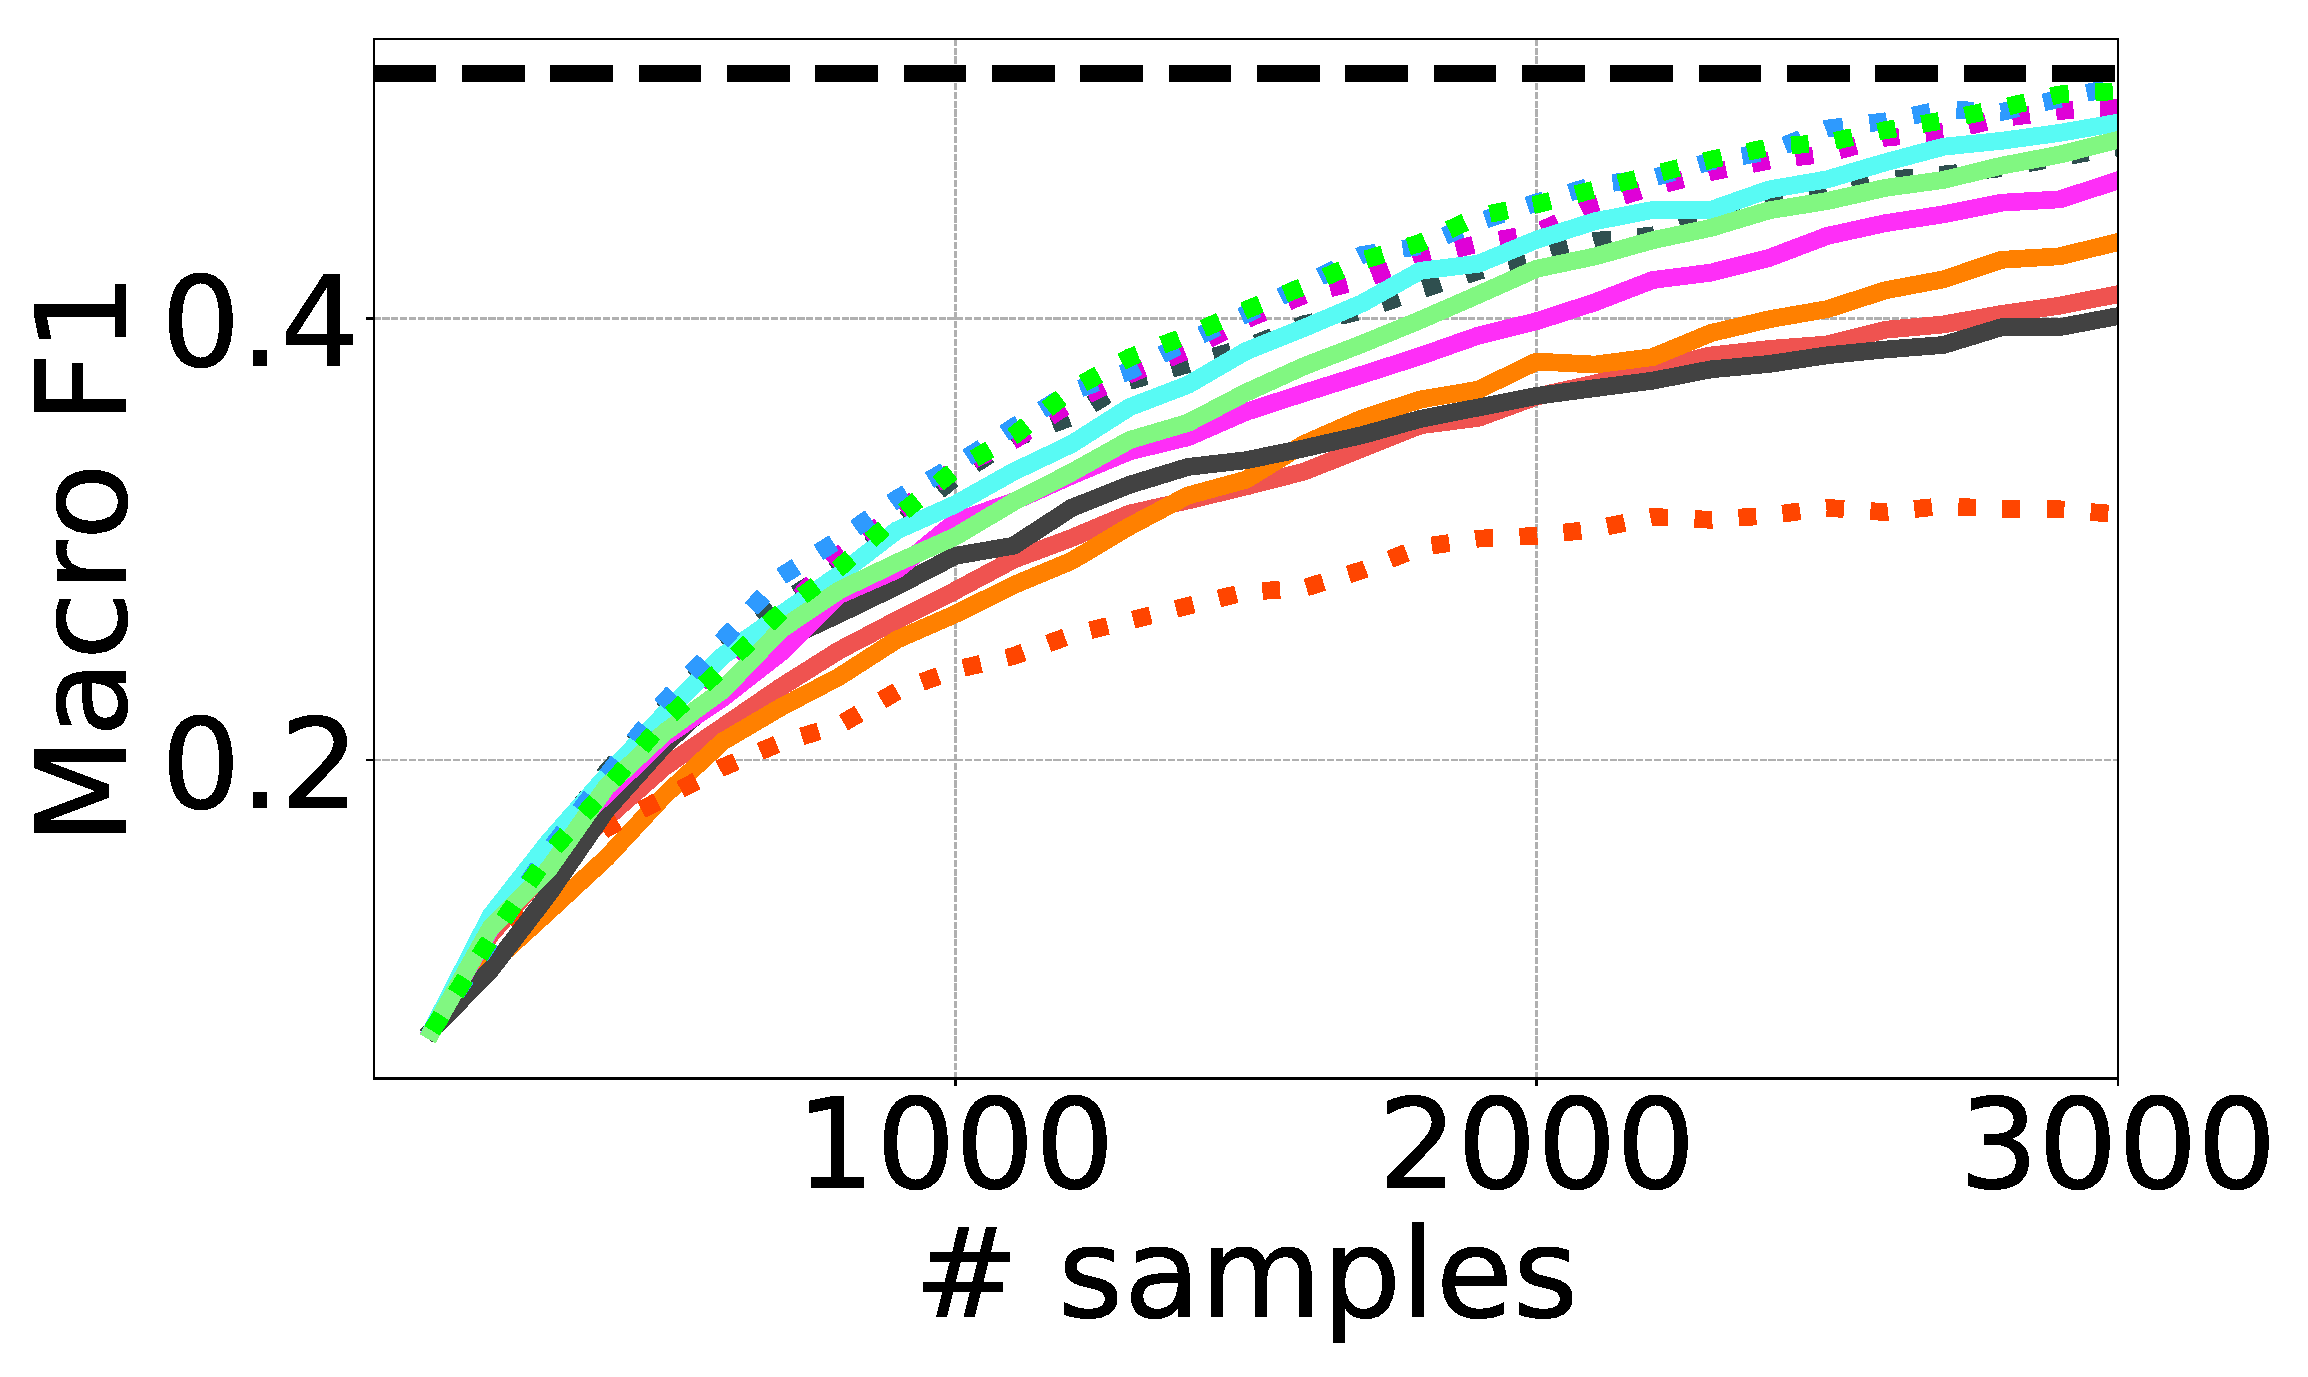
\includegraphics[width=0.23\textwidth]{res/ft_yanjing_tokenized_acc_all.eps}}
		\subfloat[Book]{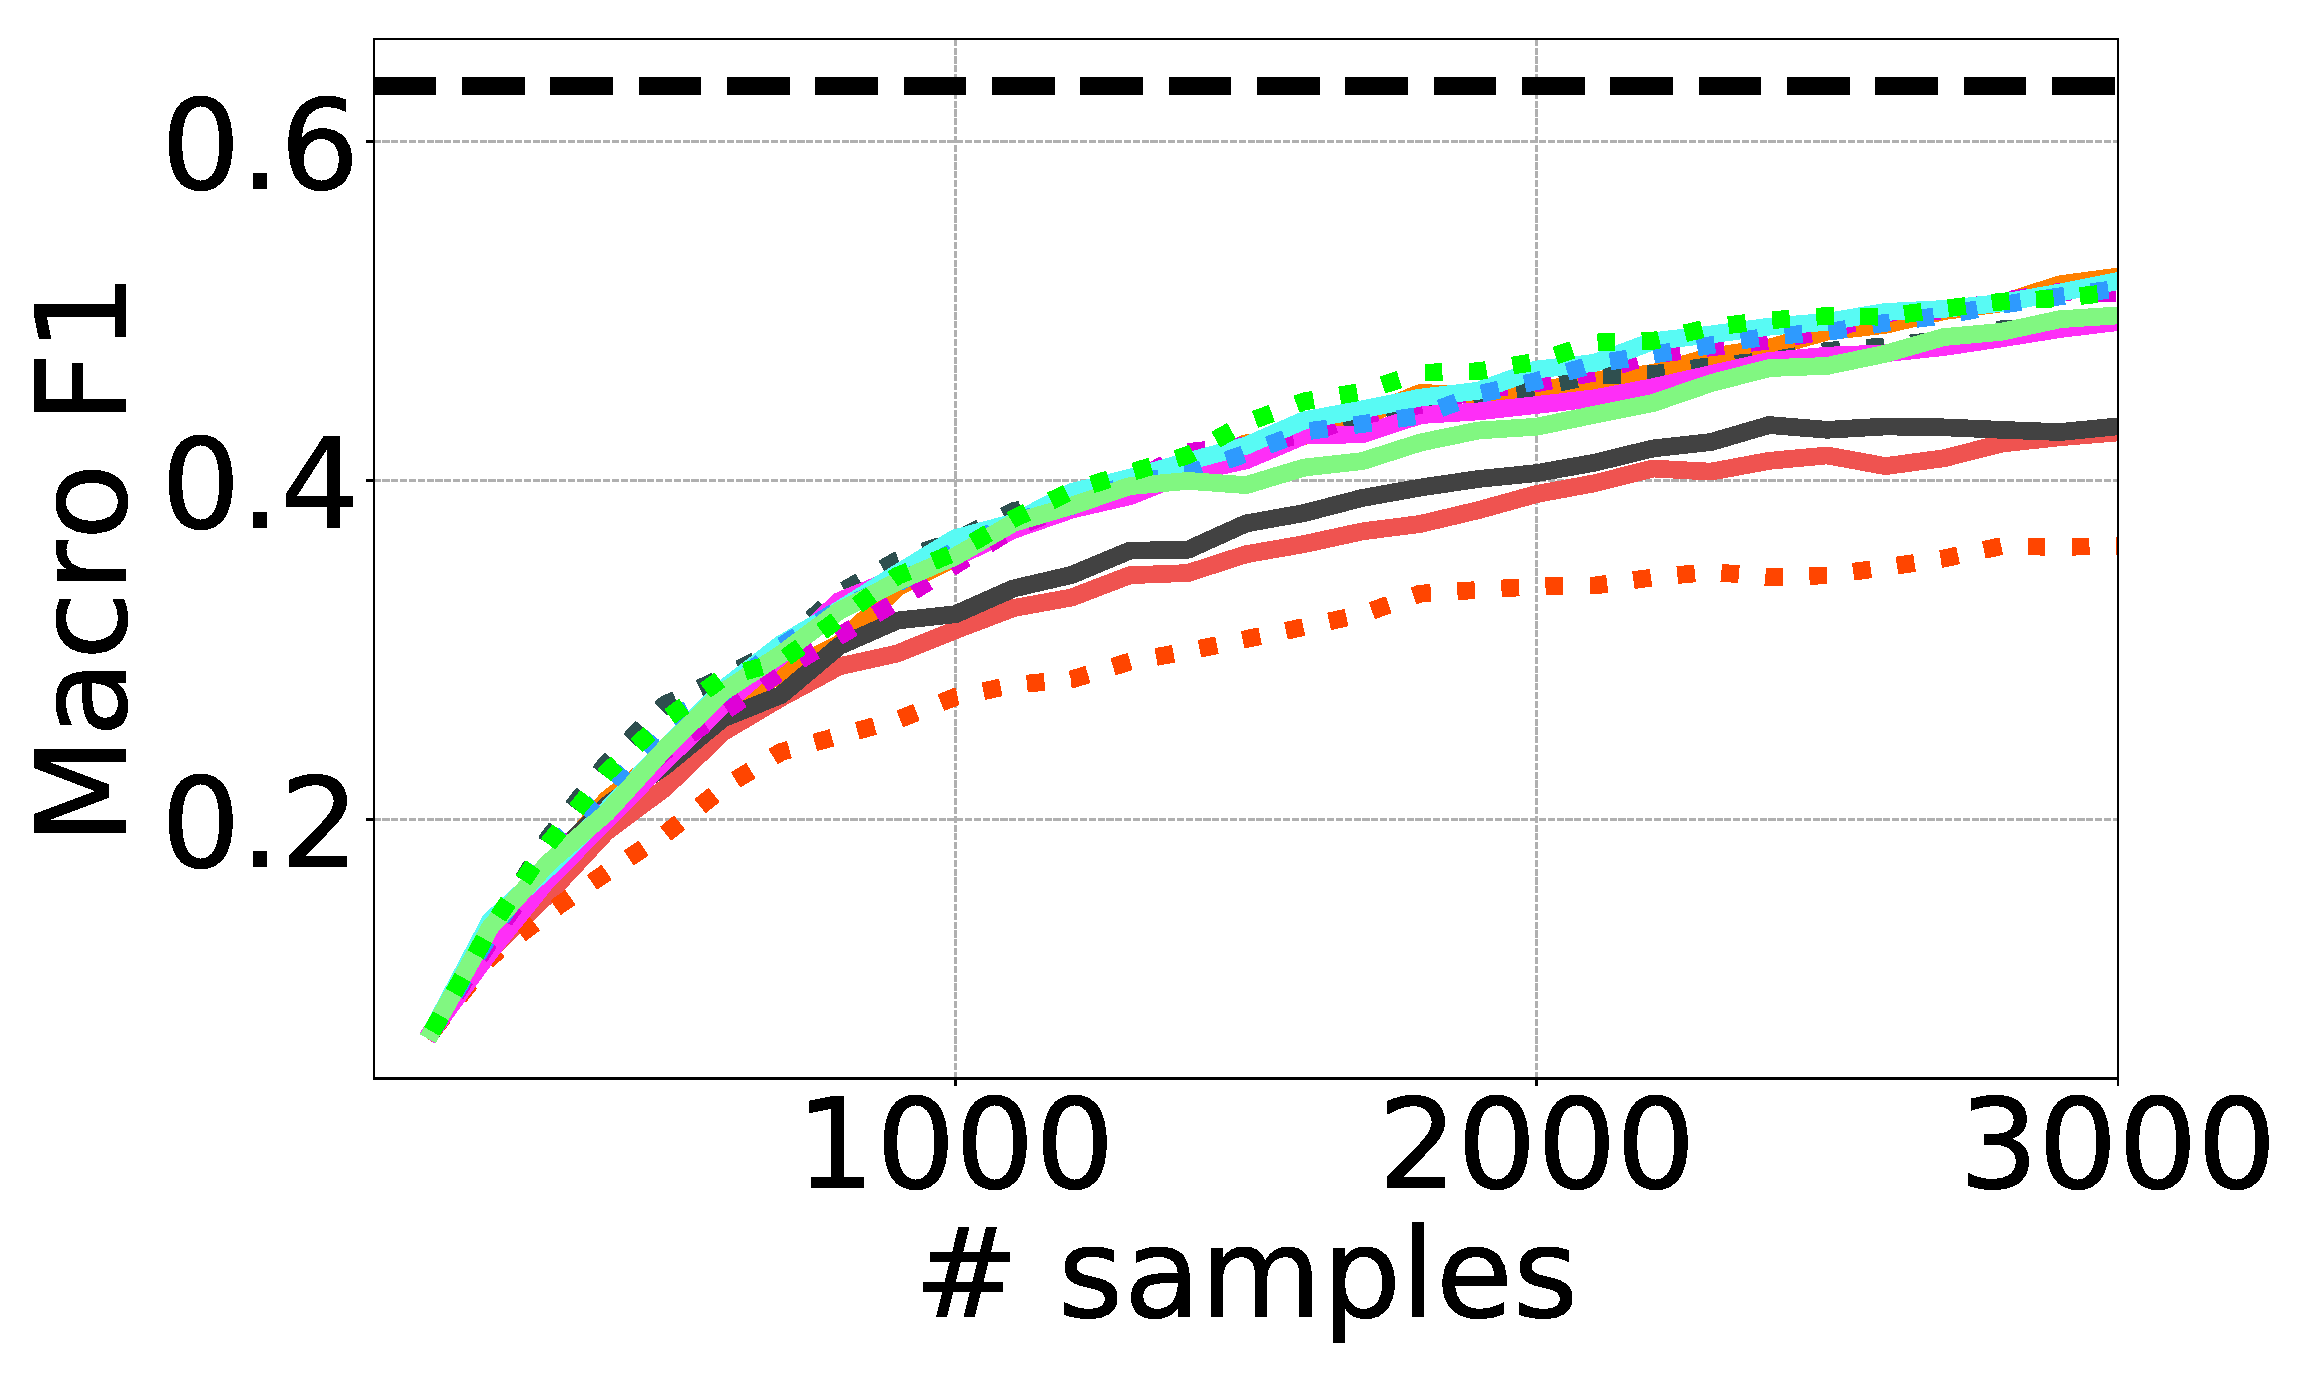
\includegraphics[width=0.23\textwidth]{res/ft_book_tokenized_acc_all.eps}}
	\end{center}
\caption{Macro F1 curve of AL approaches on 8 datasets using fastText.}
\label{fig:acc_all}
\end{figure*}


\begin{figure*}[th!]%[!hbt]
	\noindent
	\begin{center}
		\subfloat[Reuters]{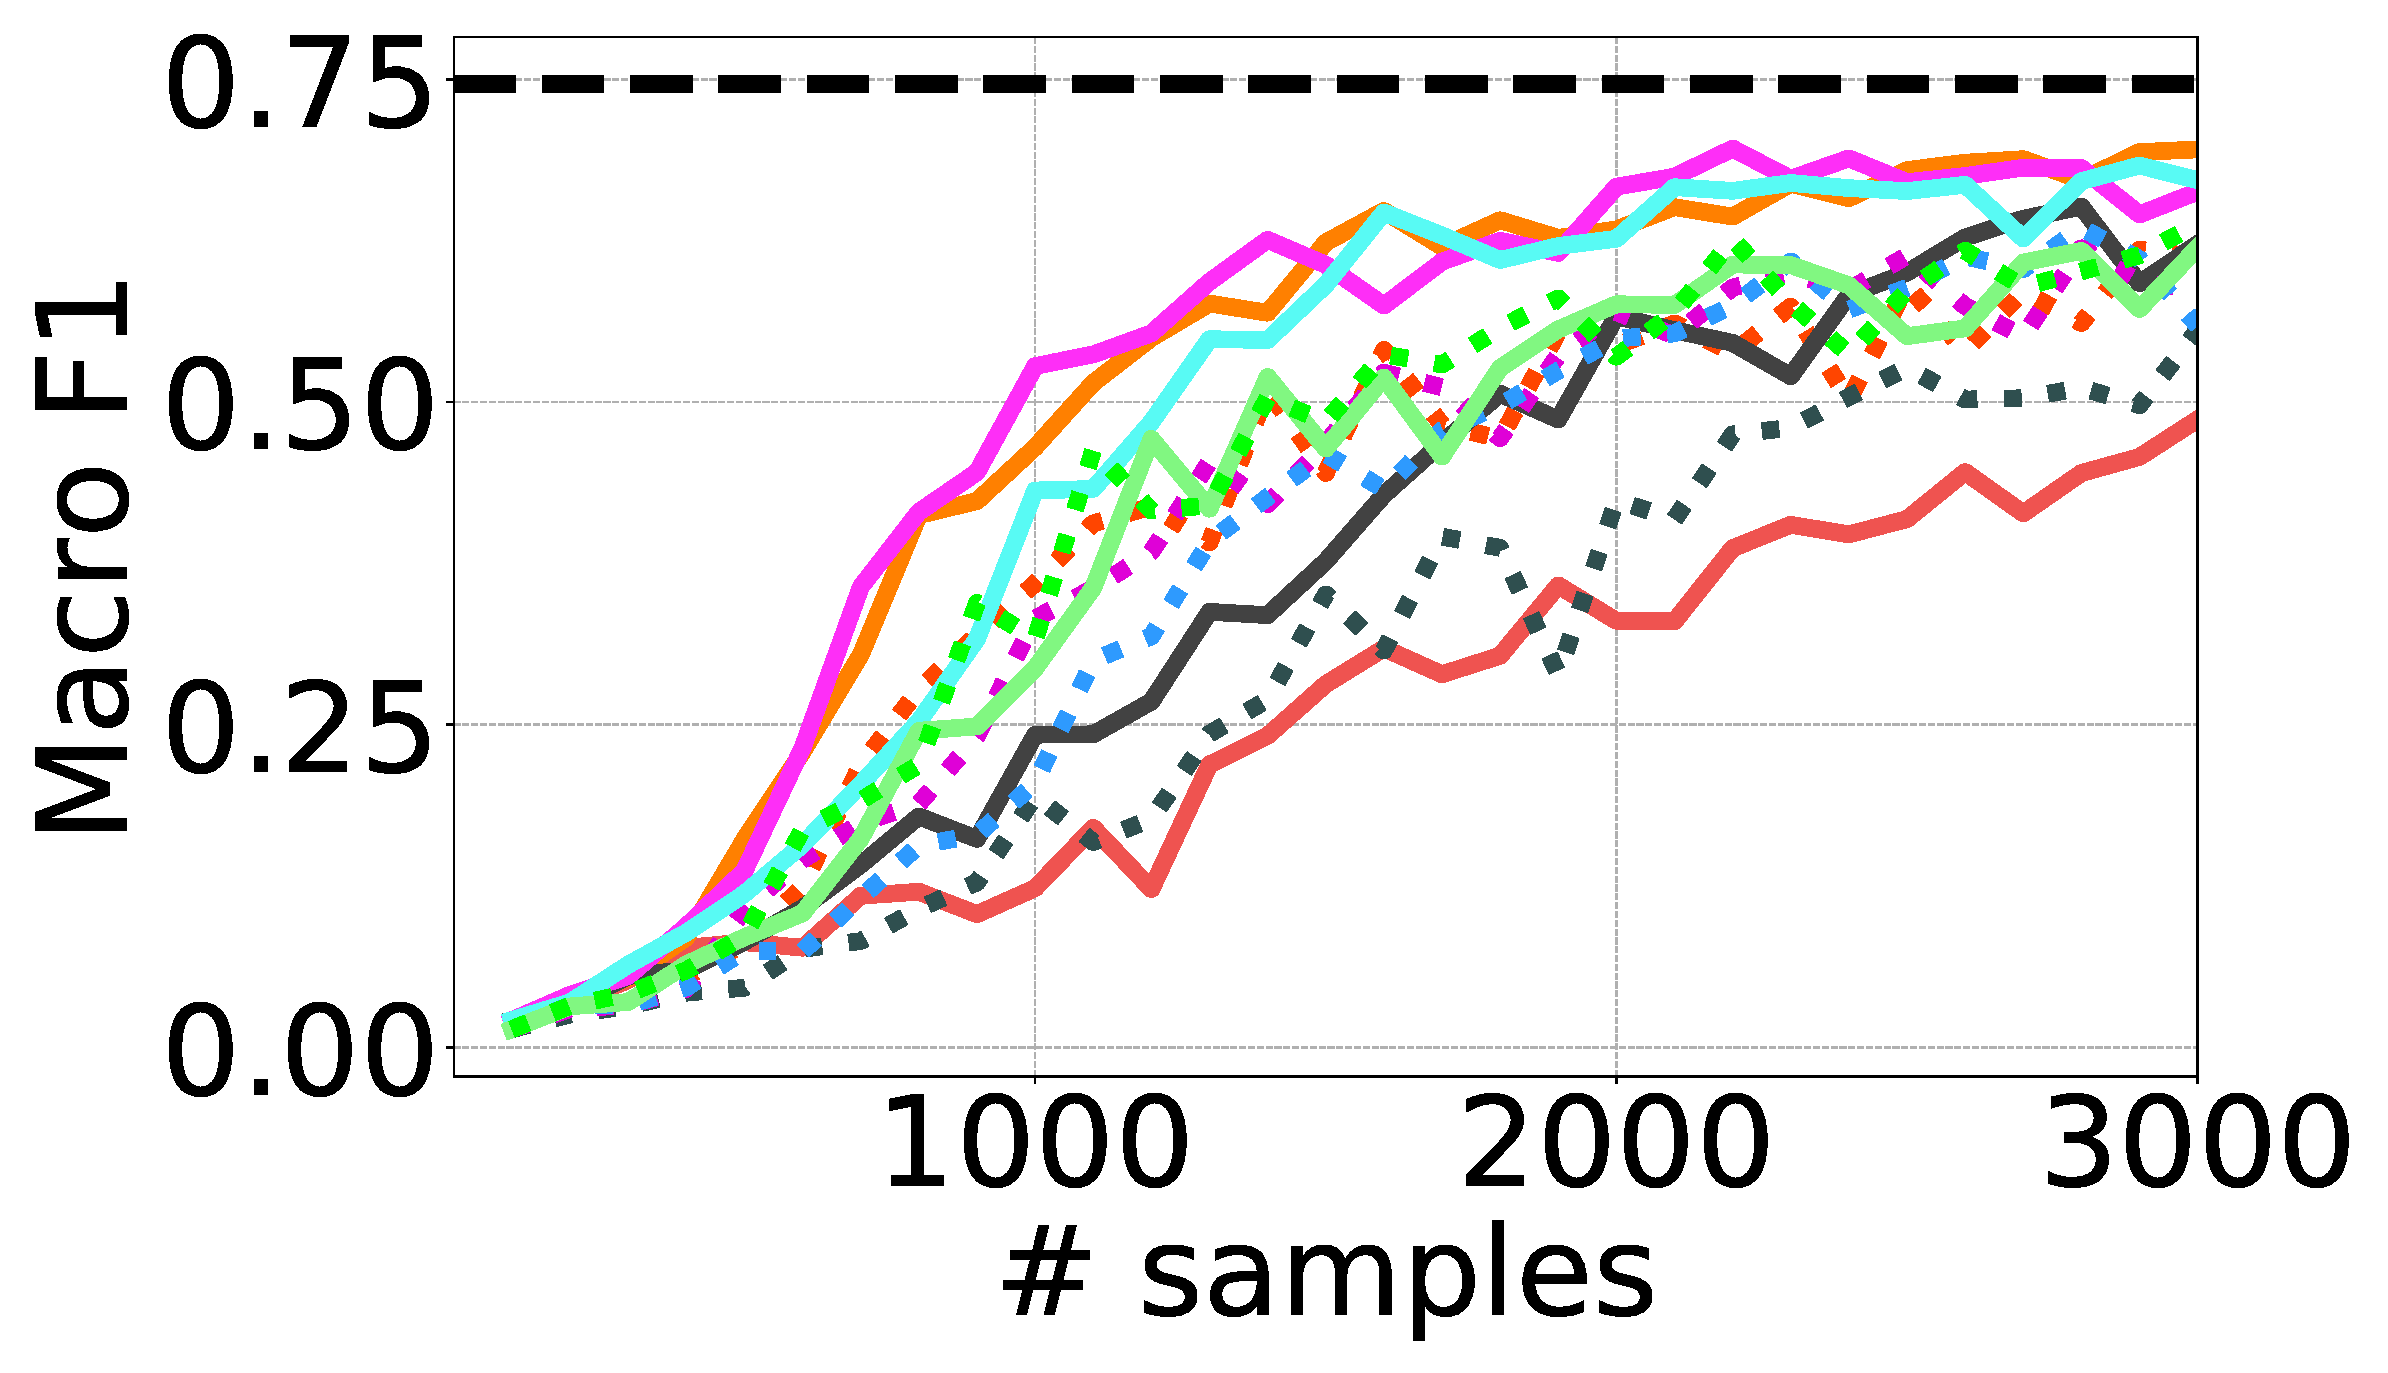
\includegraphics[width=0.23\textwidth]{figs/bert_reuters_new_epoch5_acc_all.eps}}
		\subfloat[HuffPost]{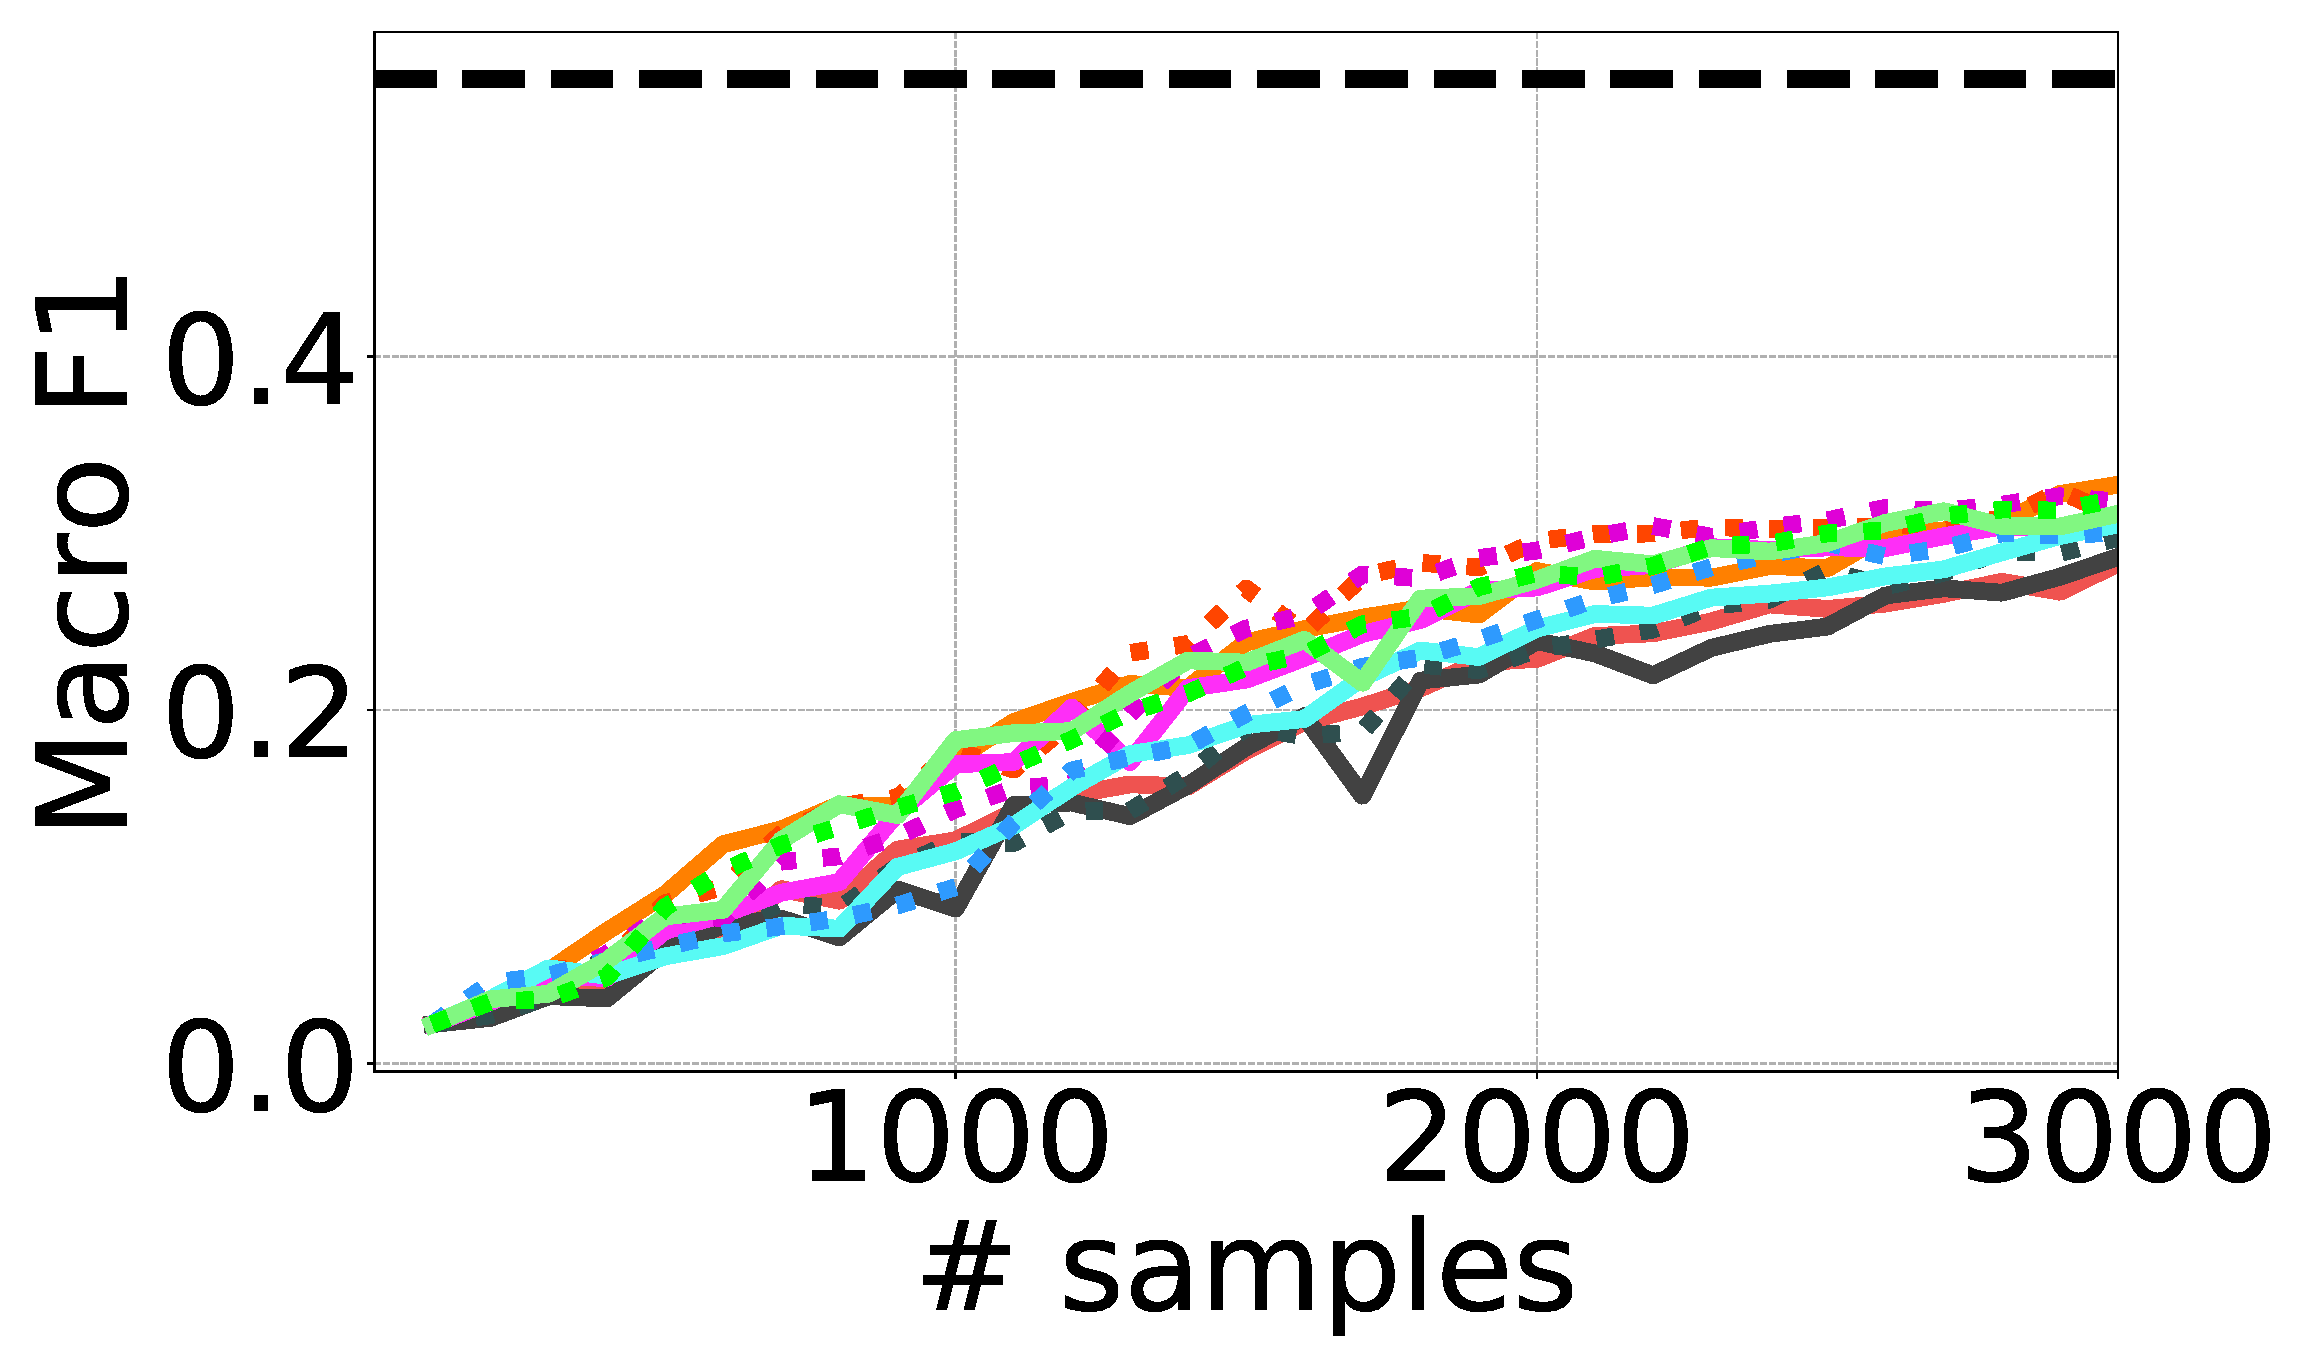
\includegraphics[width=0.23\textwidth]{figs/bert_news_epoch5_acc_all.eps}}
		\subfloat[Biomedical]{\includegraphics[width=0.23\textwidth]{figs/bert_Bio_epoch5_run1_acc_all.eps}}
		\subfloat[SearchSnippets]{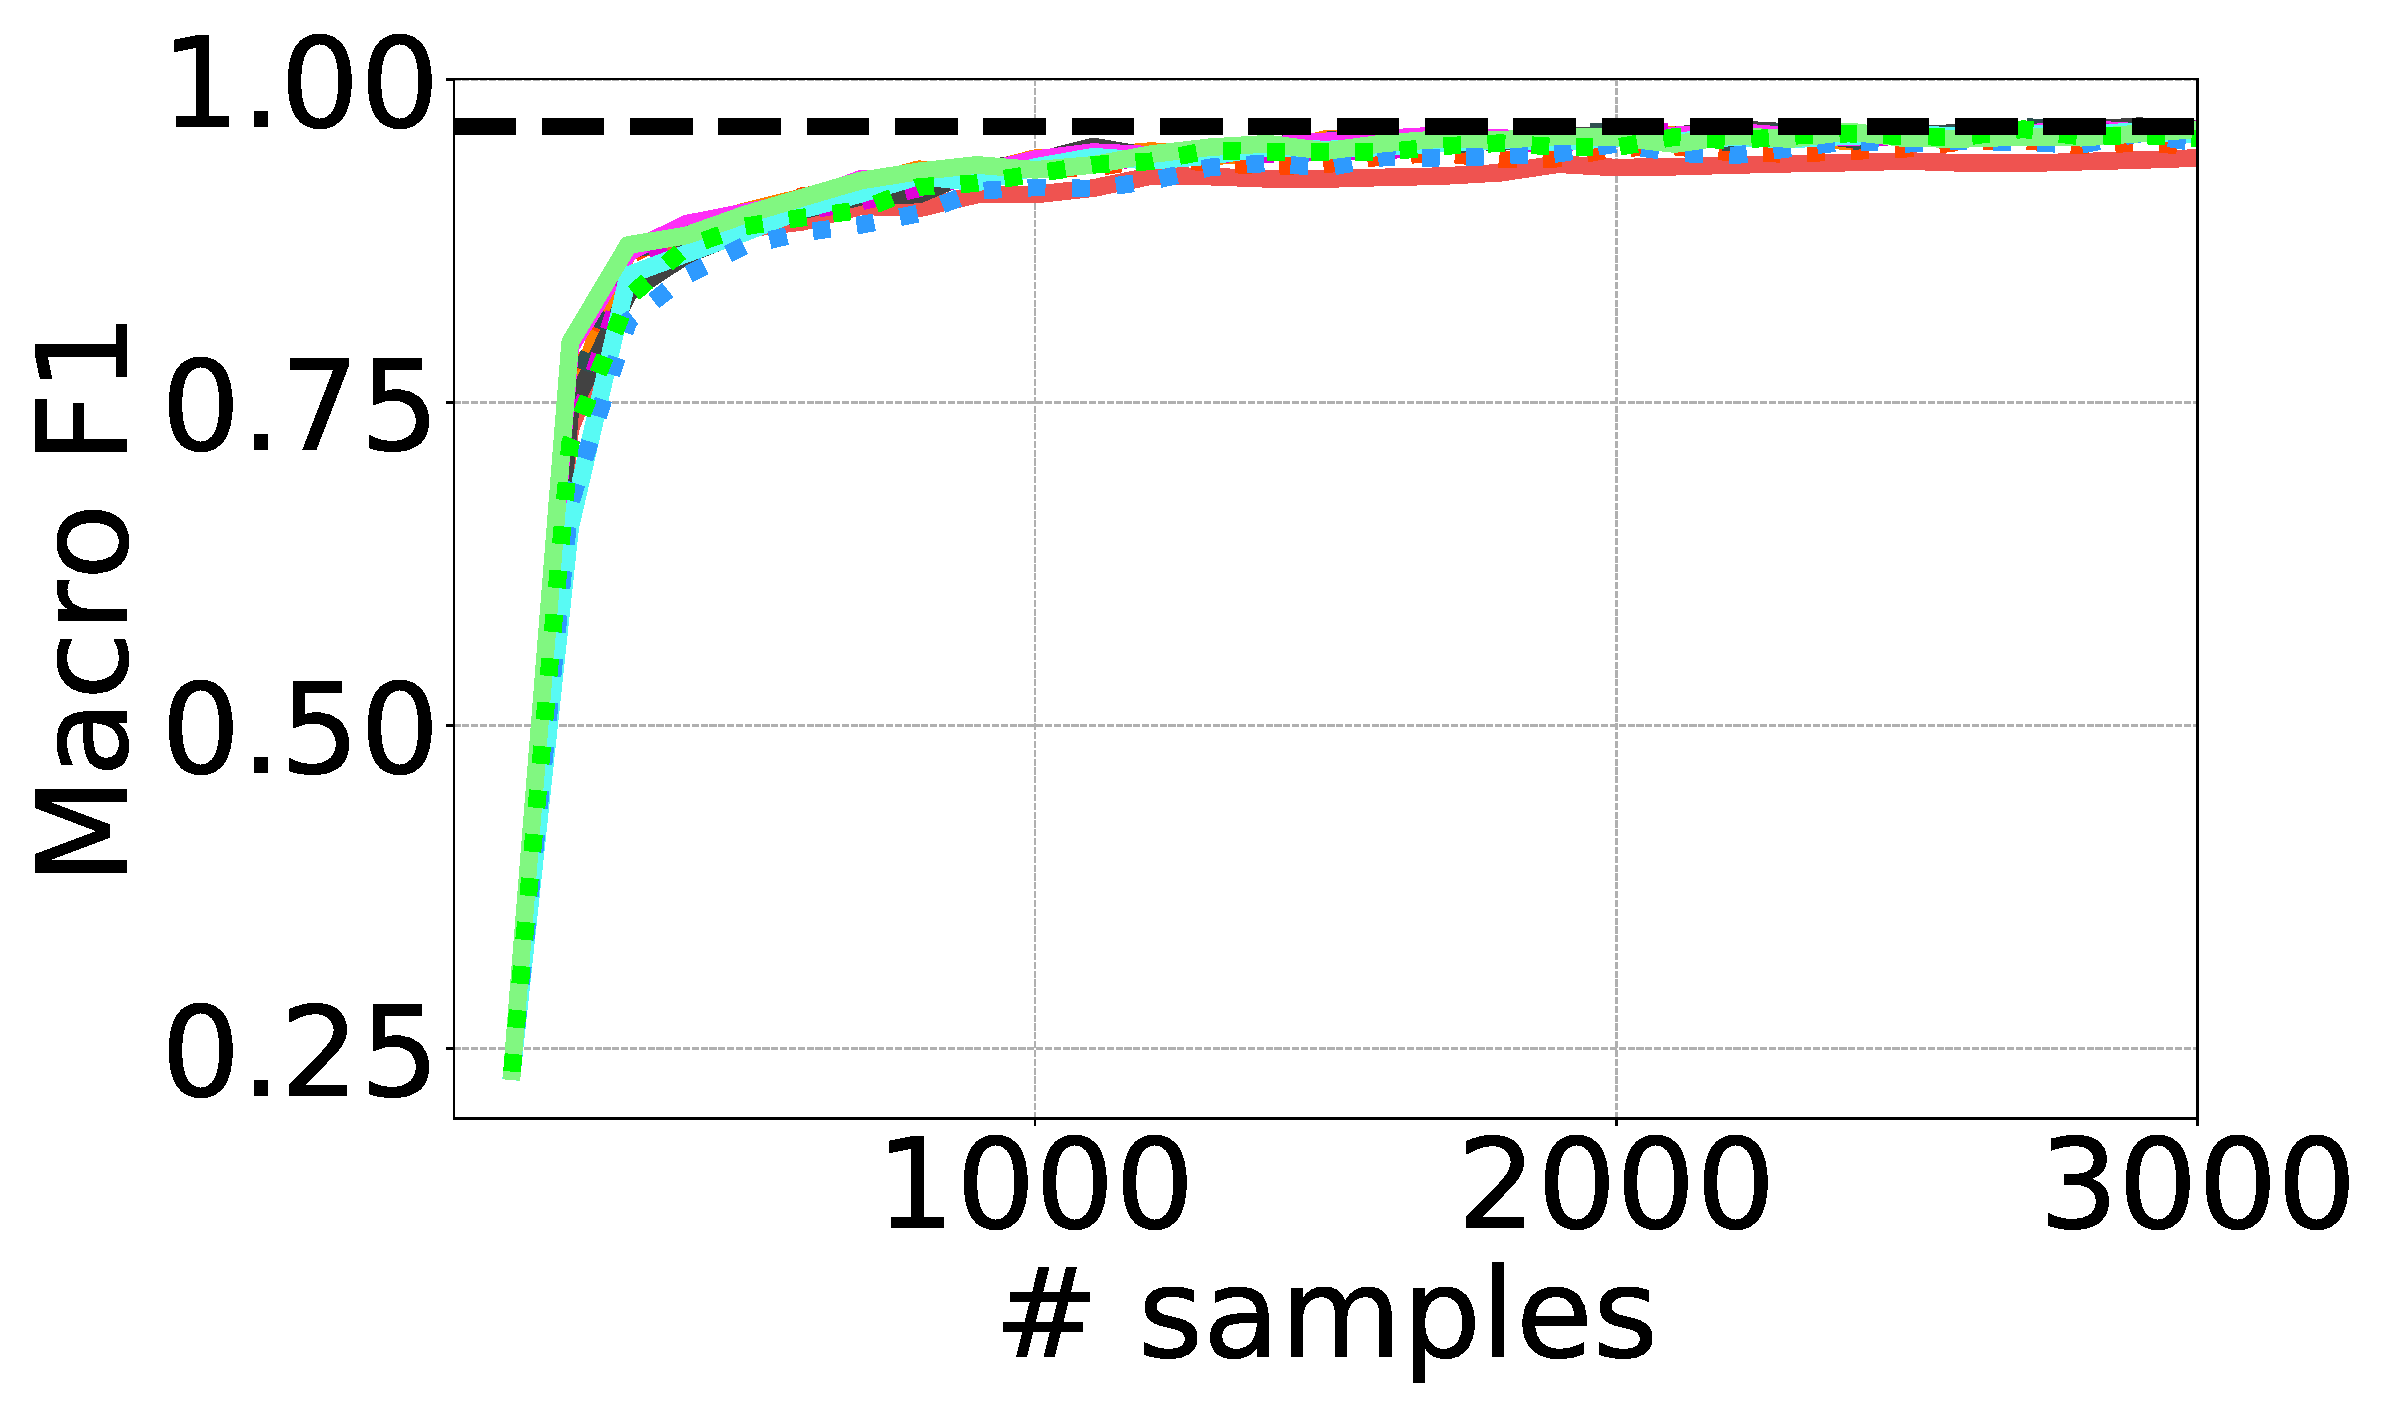
\includegraphics[width=0.23\textwidth]{figs/bert_Search_epoch5_run1_acc_all.eps}}
	\end{center}
	\noindent
	\begin{center}
		\subfloat[Emoji]{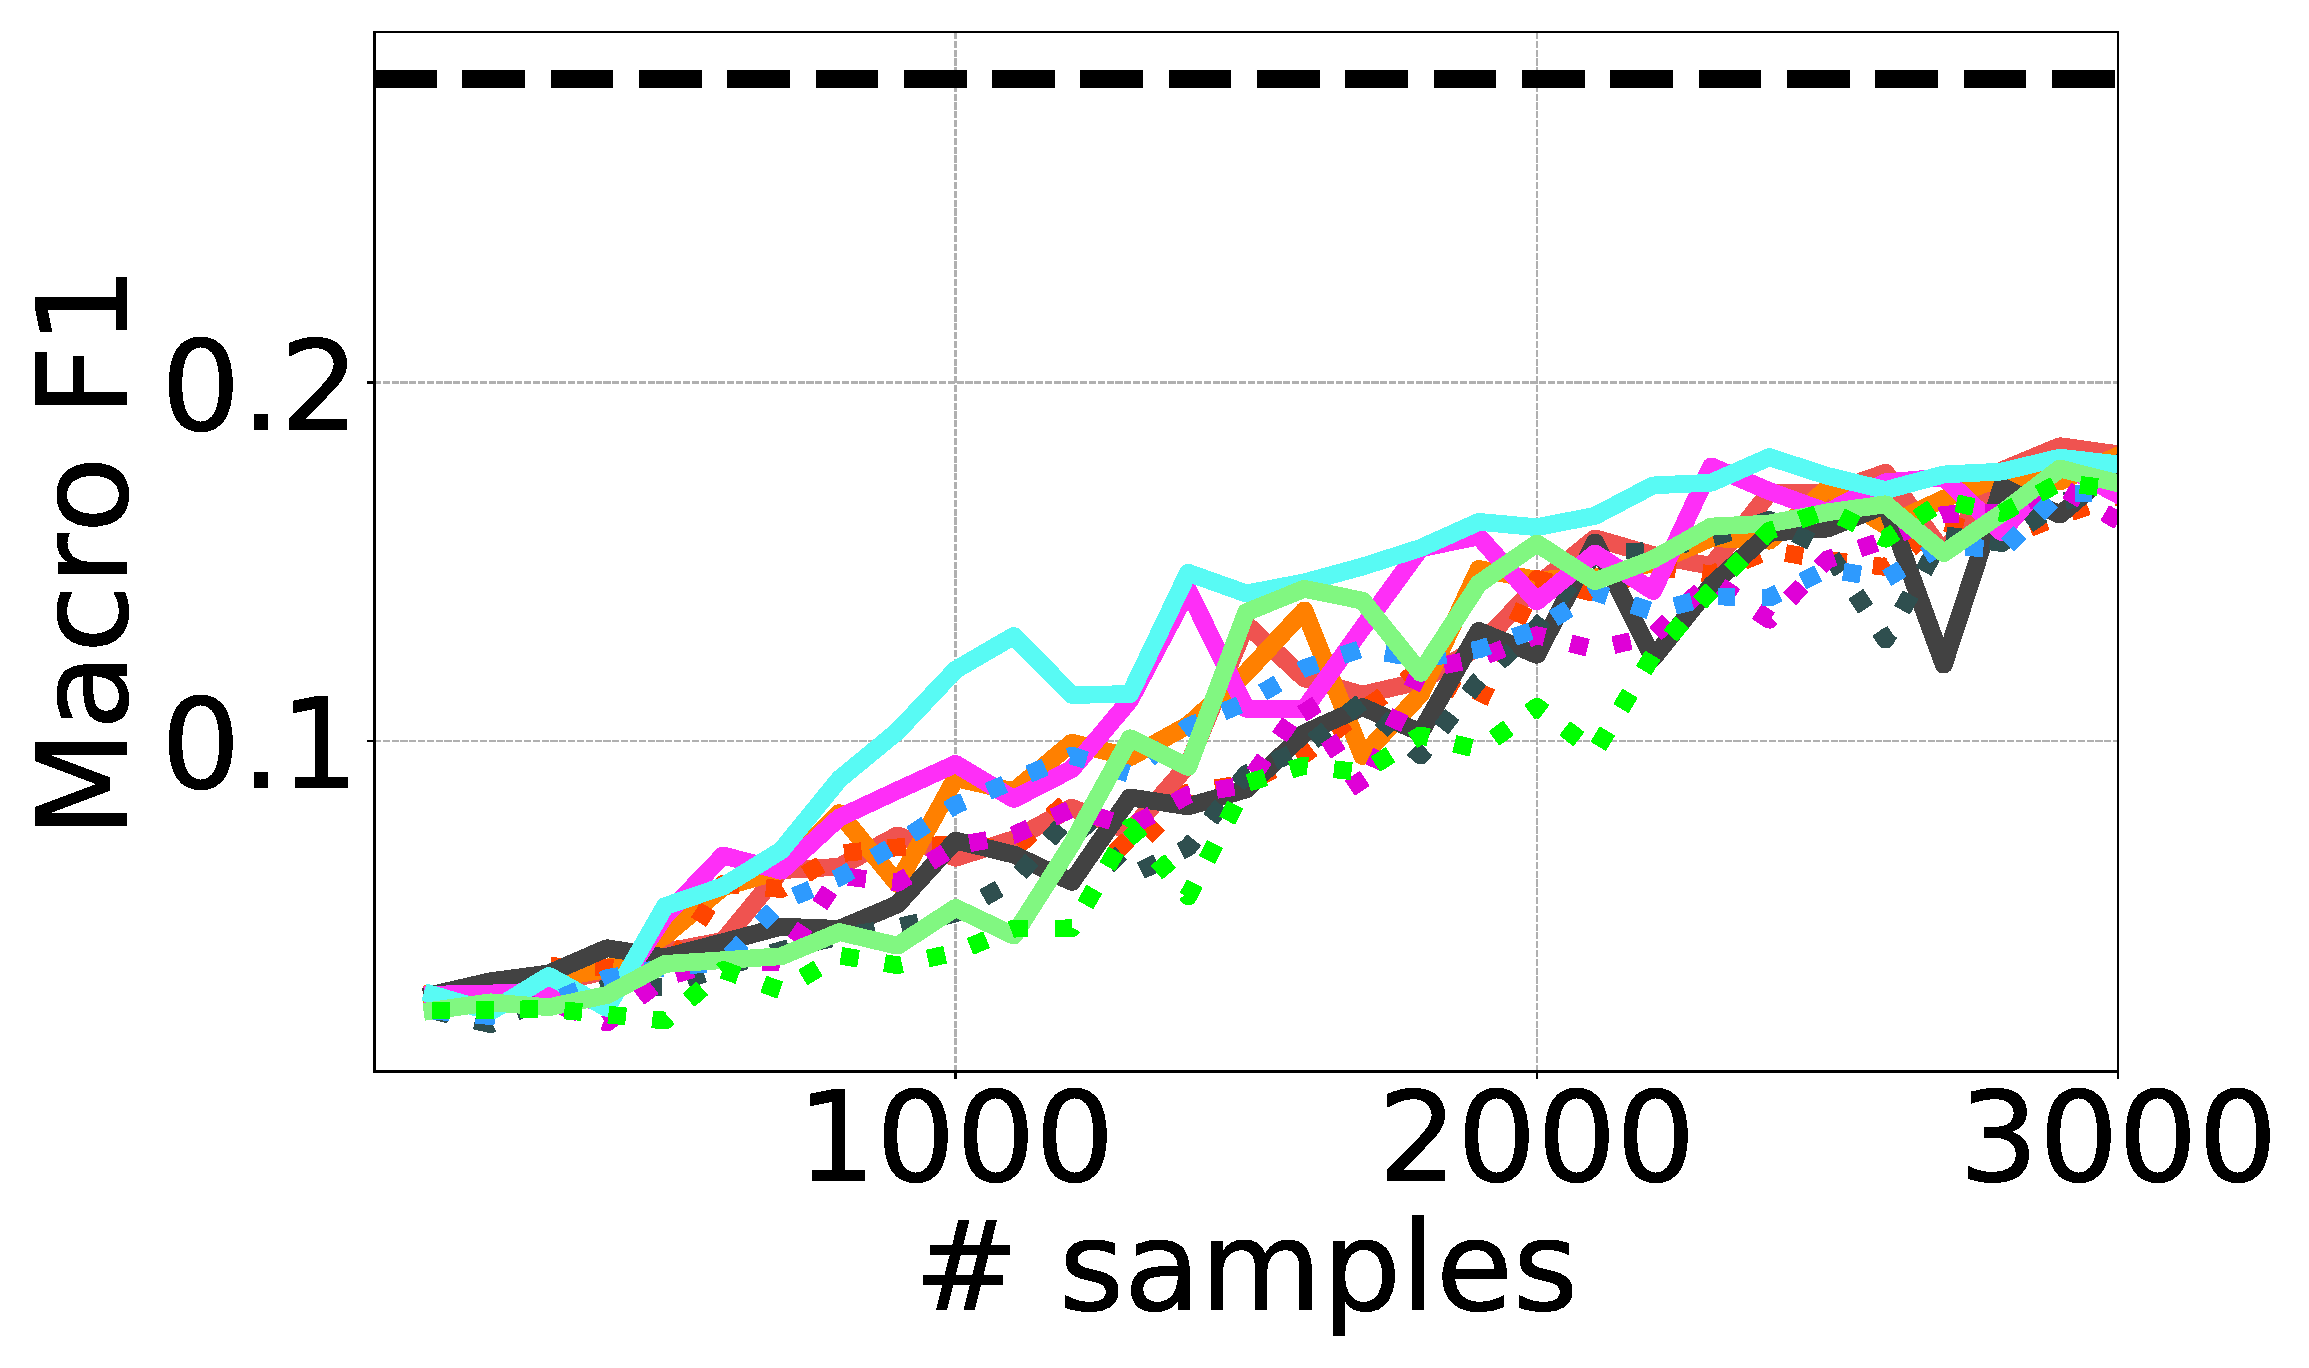
\includegraphics[width=0.23\textwidth]{figs/bert_emoji_epoch5_run1_acc_all.eps}}
		\subfloat[TNEWS]{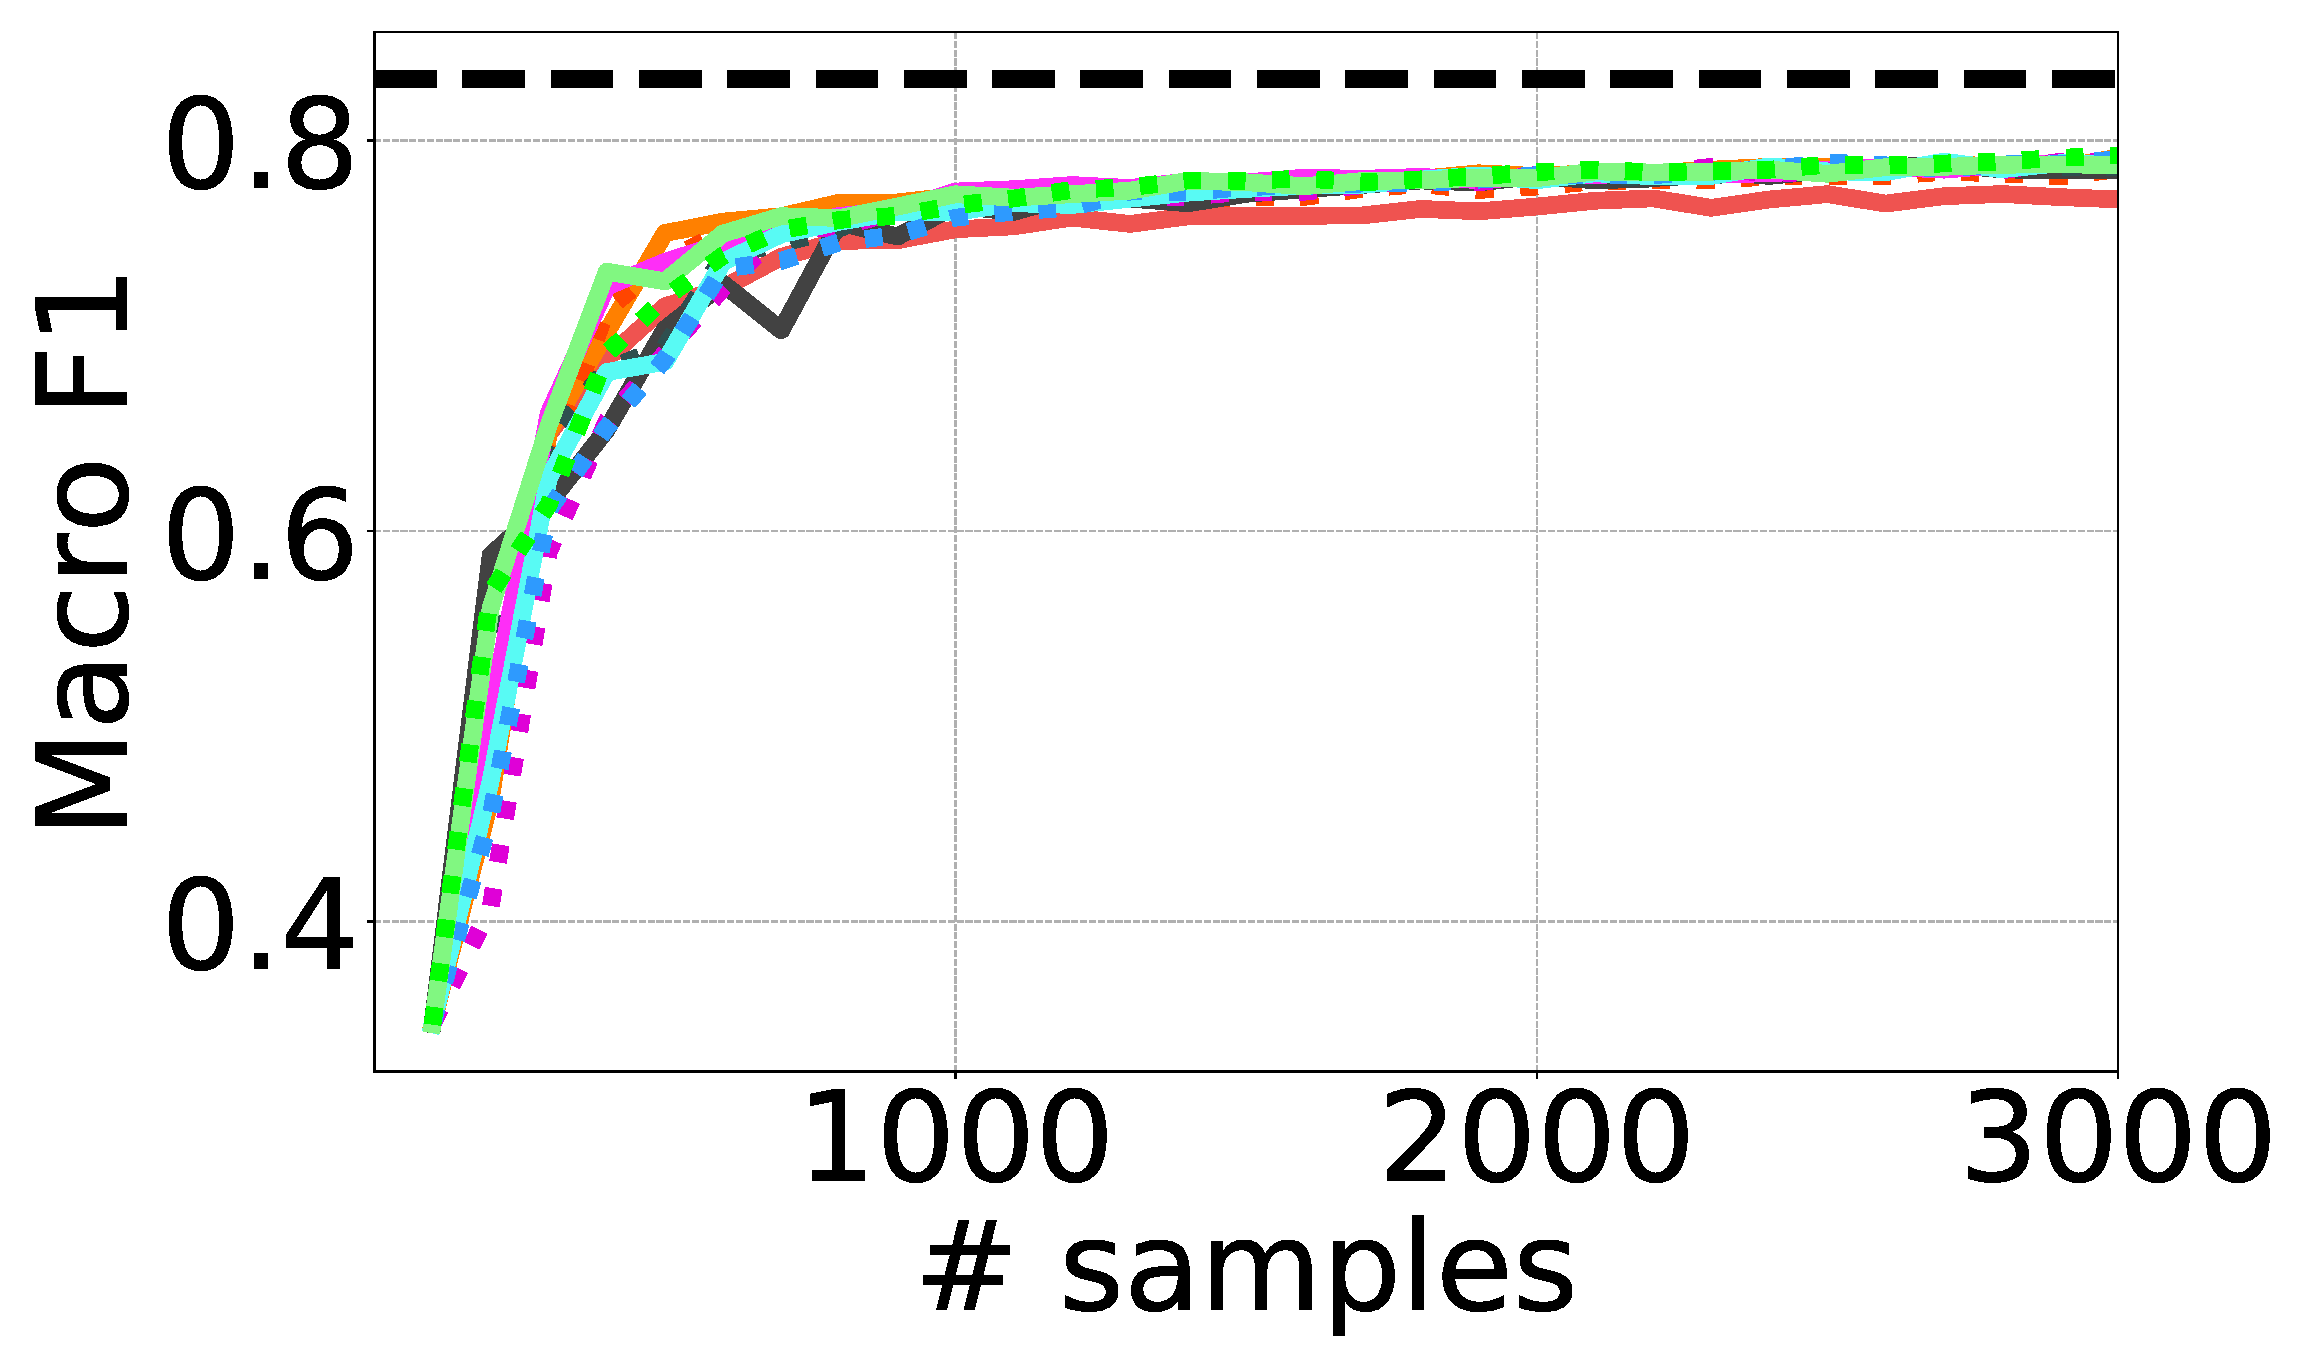
\includegraphics[width=0.23\textwidth]{figs/bert_tnews_epoch5_acc_all.eps}}
		\subfloat[GCS]{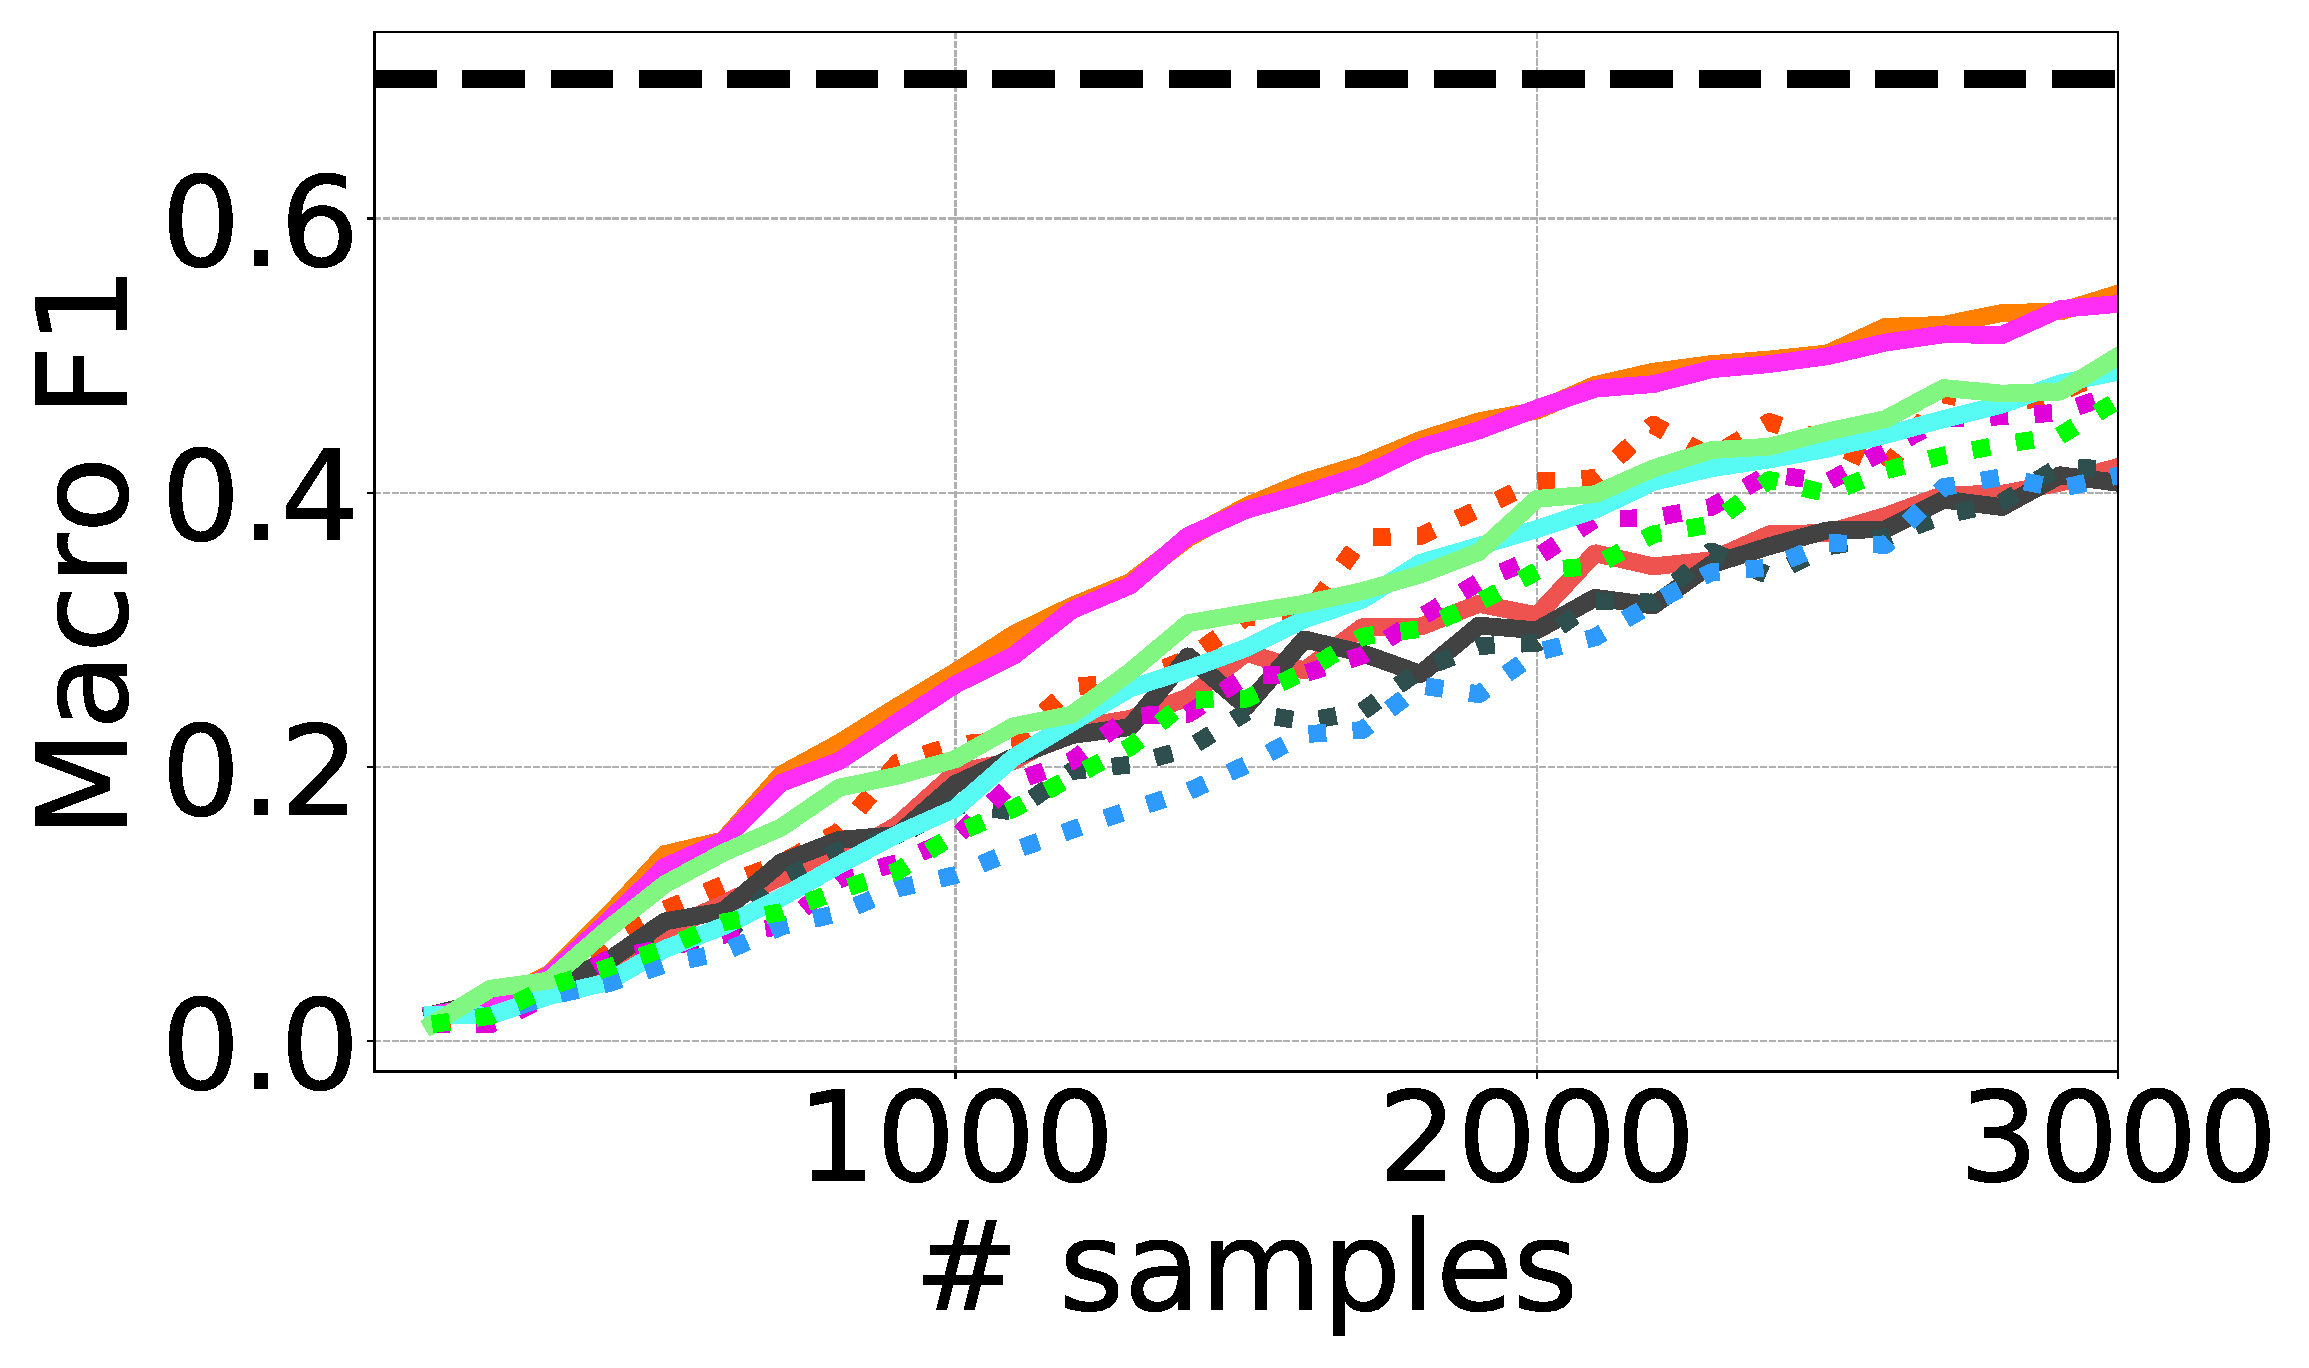
\includegraphics[width=0.23\textwidth]{figs/bert_yanjing_epoch5_acc_all.eps}}
		\subfloat[Book]{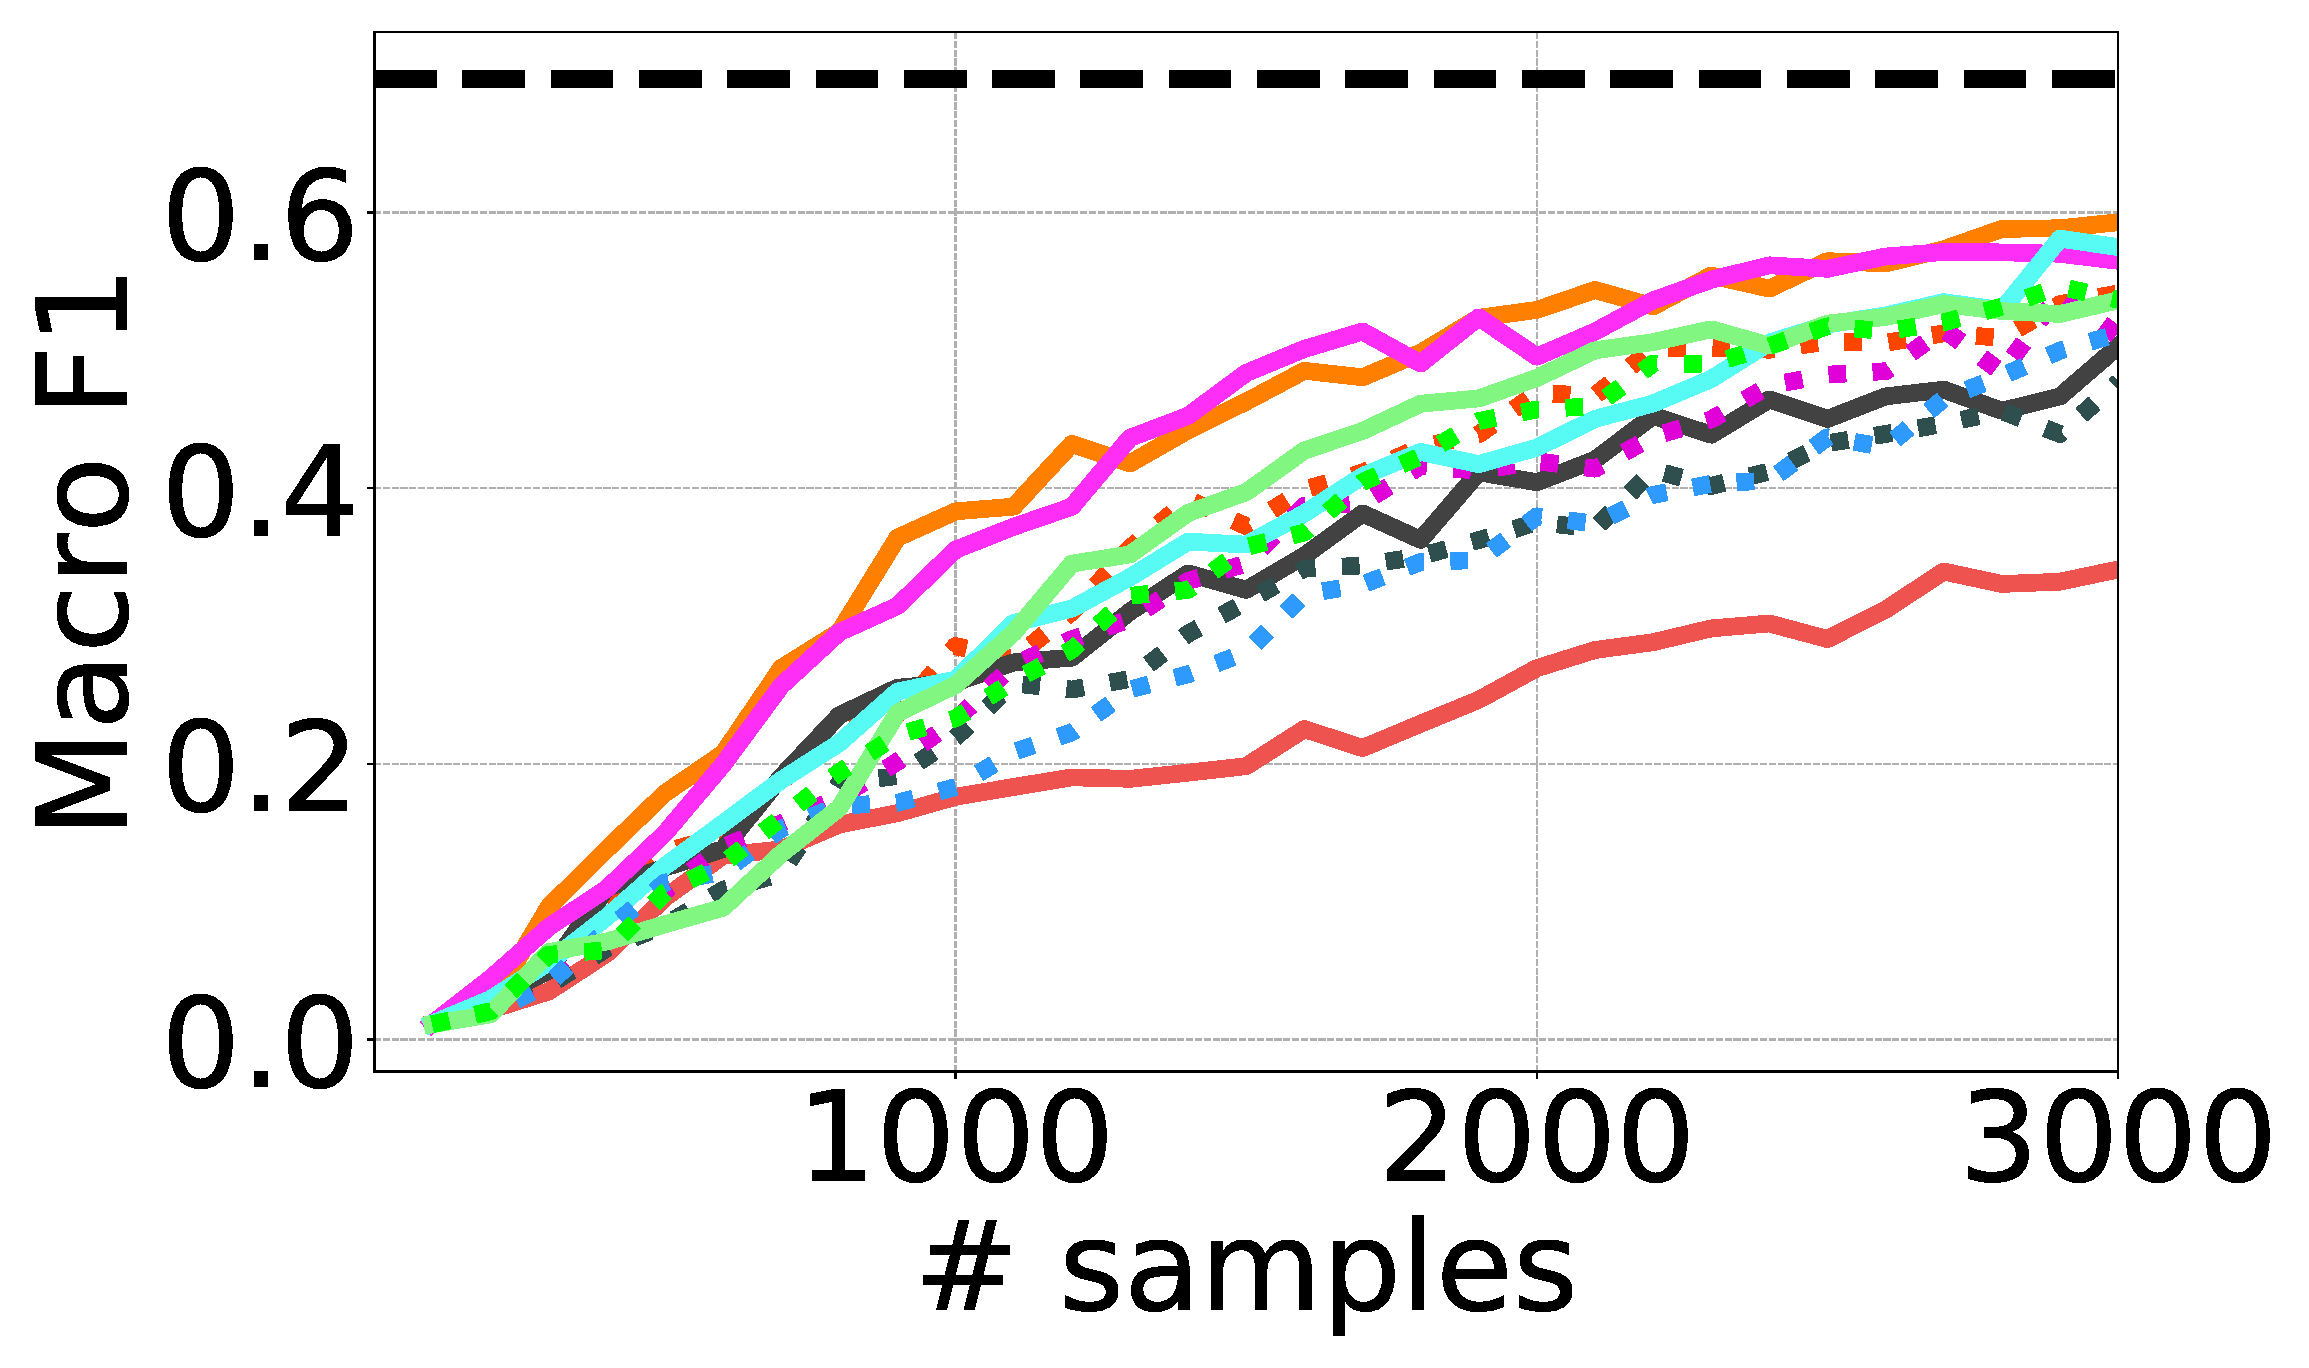
\includegraphics[width=0.23\textwidth]{figs/bert_book_epoch5_run1_acc_all.eps}}
	\end{center}

	\caption{Macro F1 curve of AL approaches on 8 datasets using BERT.}
	\label{fig:acc_all_bert}
\end{figure*}

\begin{figure*}[th!]%[!hbt]
	\noindent
	\begin{center}
		\subfloat[Reuters]{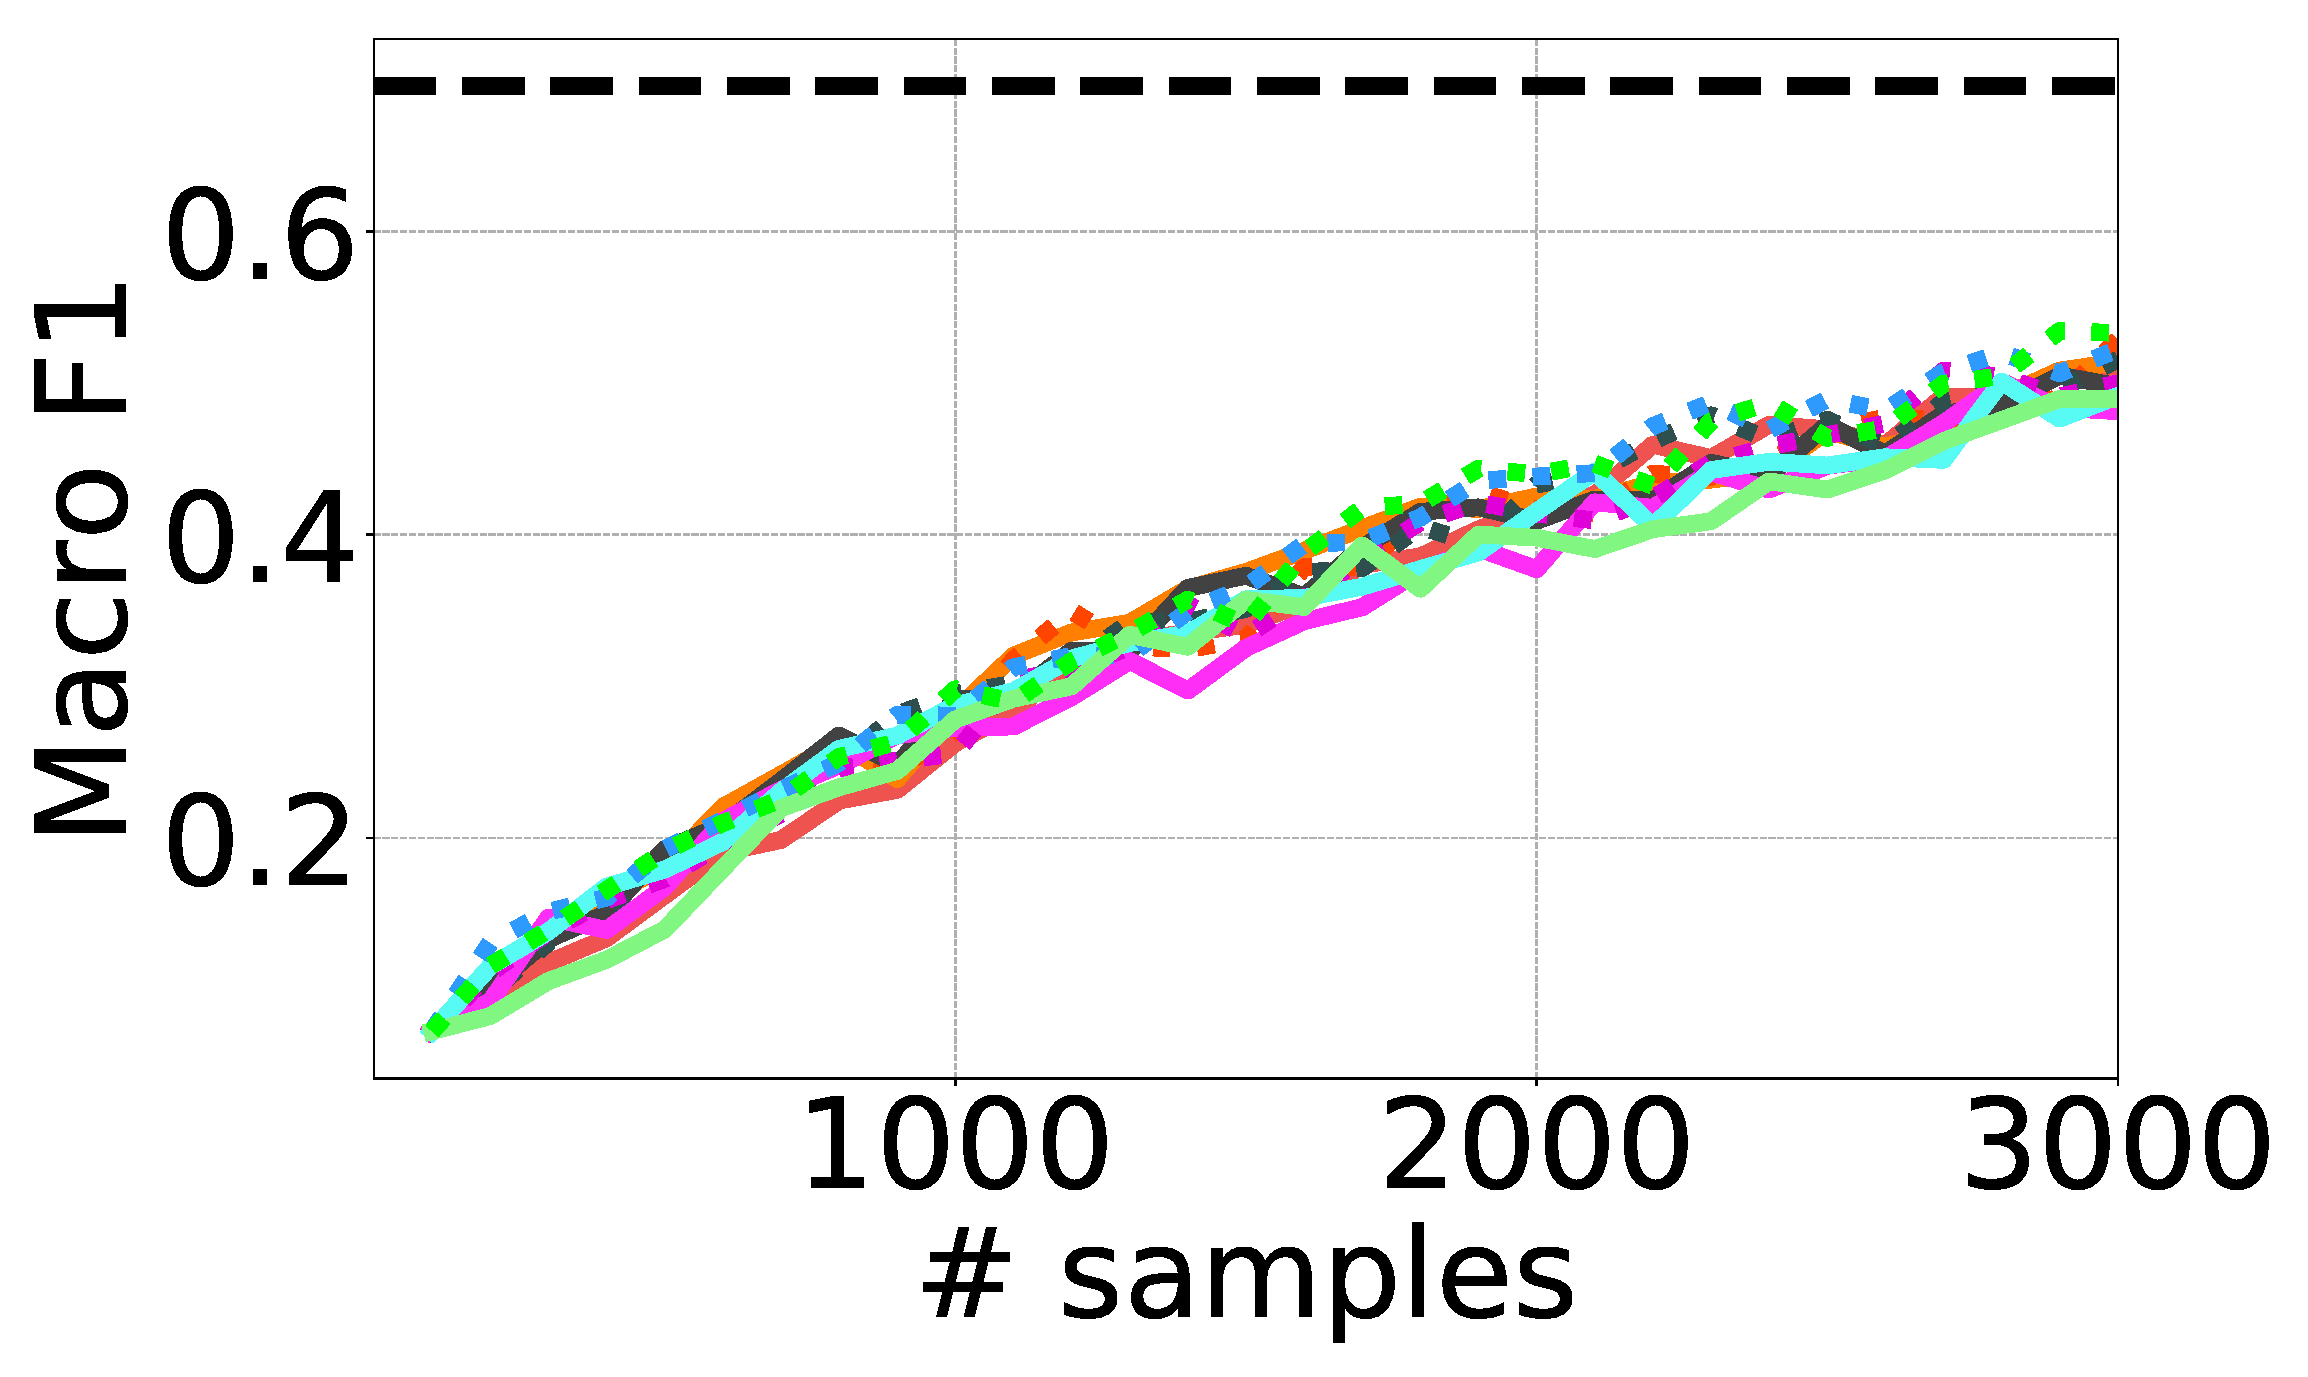
\includegraphics[width=0.23\textwidth]{res/lstm_pytorch_reuters_new_acc_all.eps}}
		\subfloat[HuffPost]{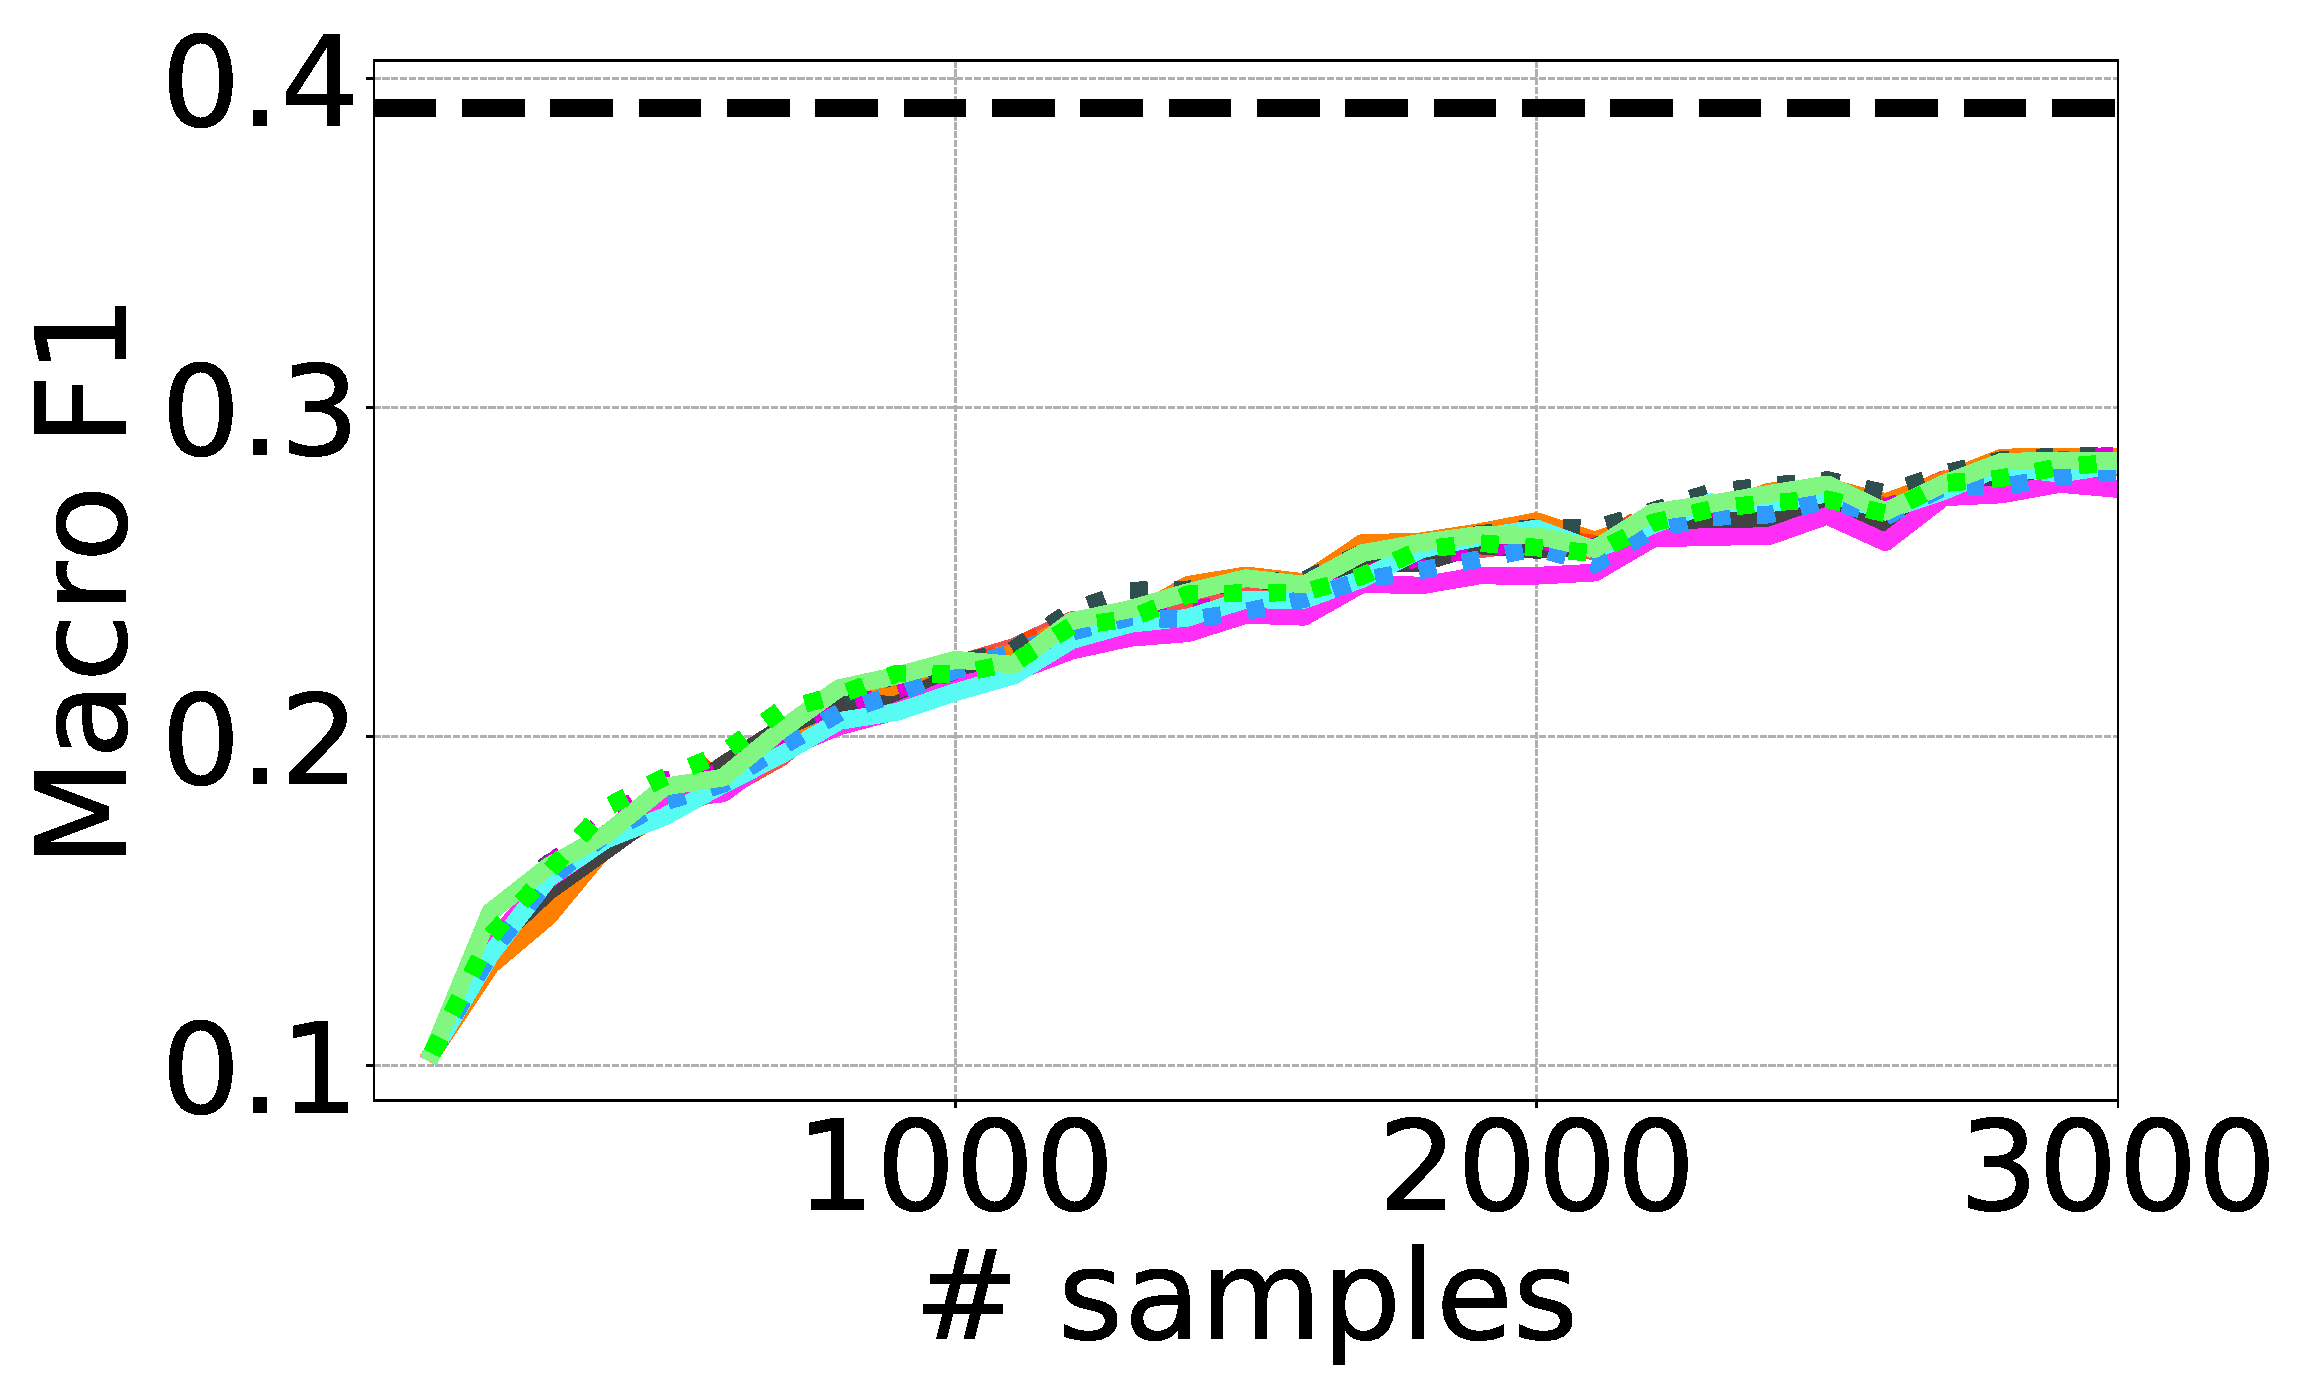
\includegraphics[width=0.23\textwidth]{res/lstm_pytorch_news_reshuffle_tokenized_acc_all.eps}}
		\subfloat[Biomedical]{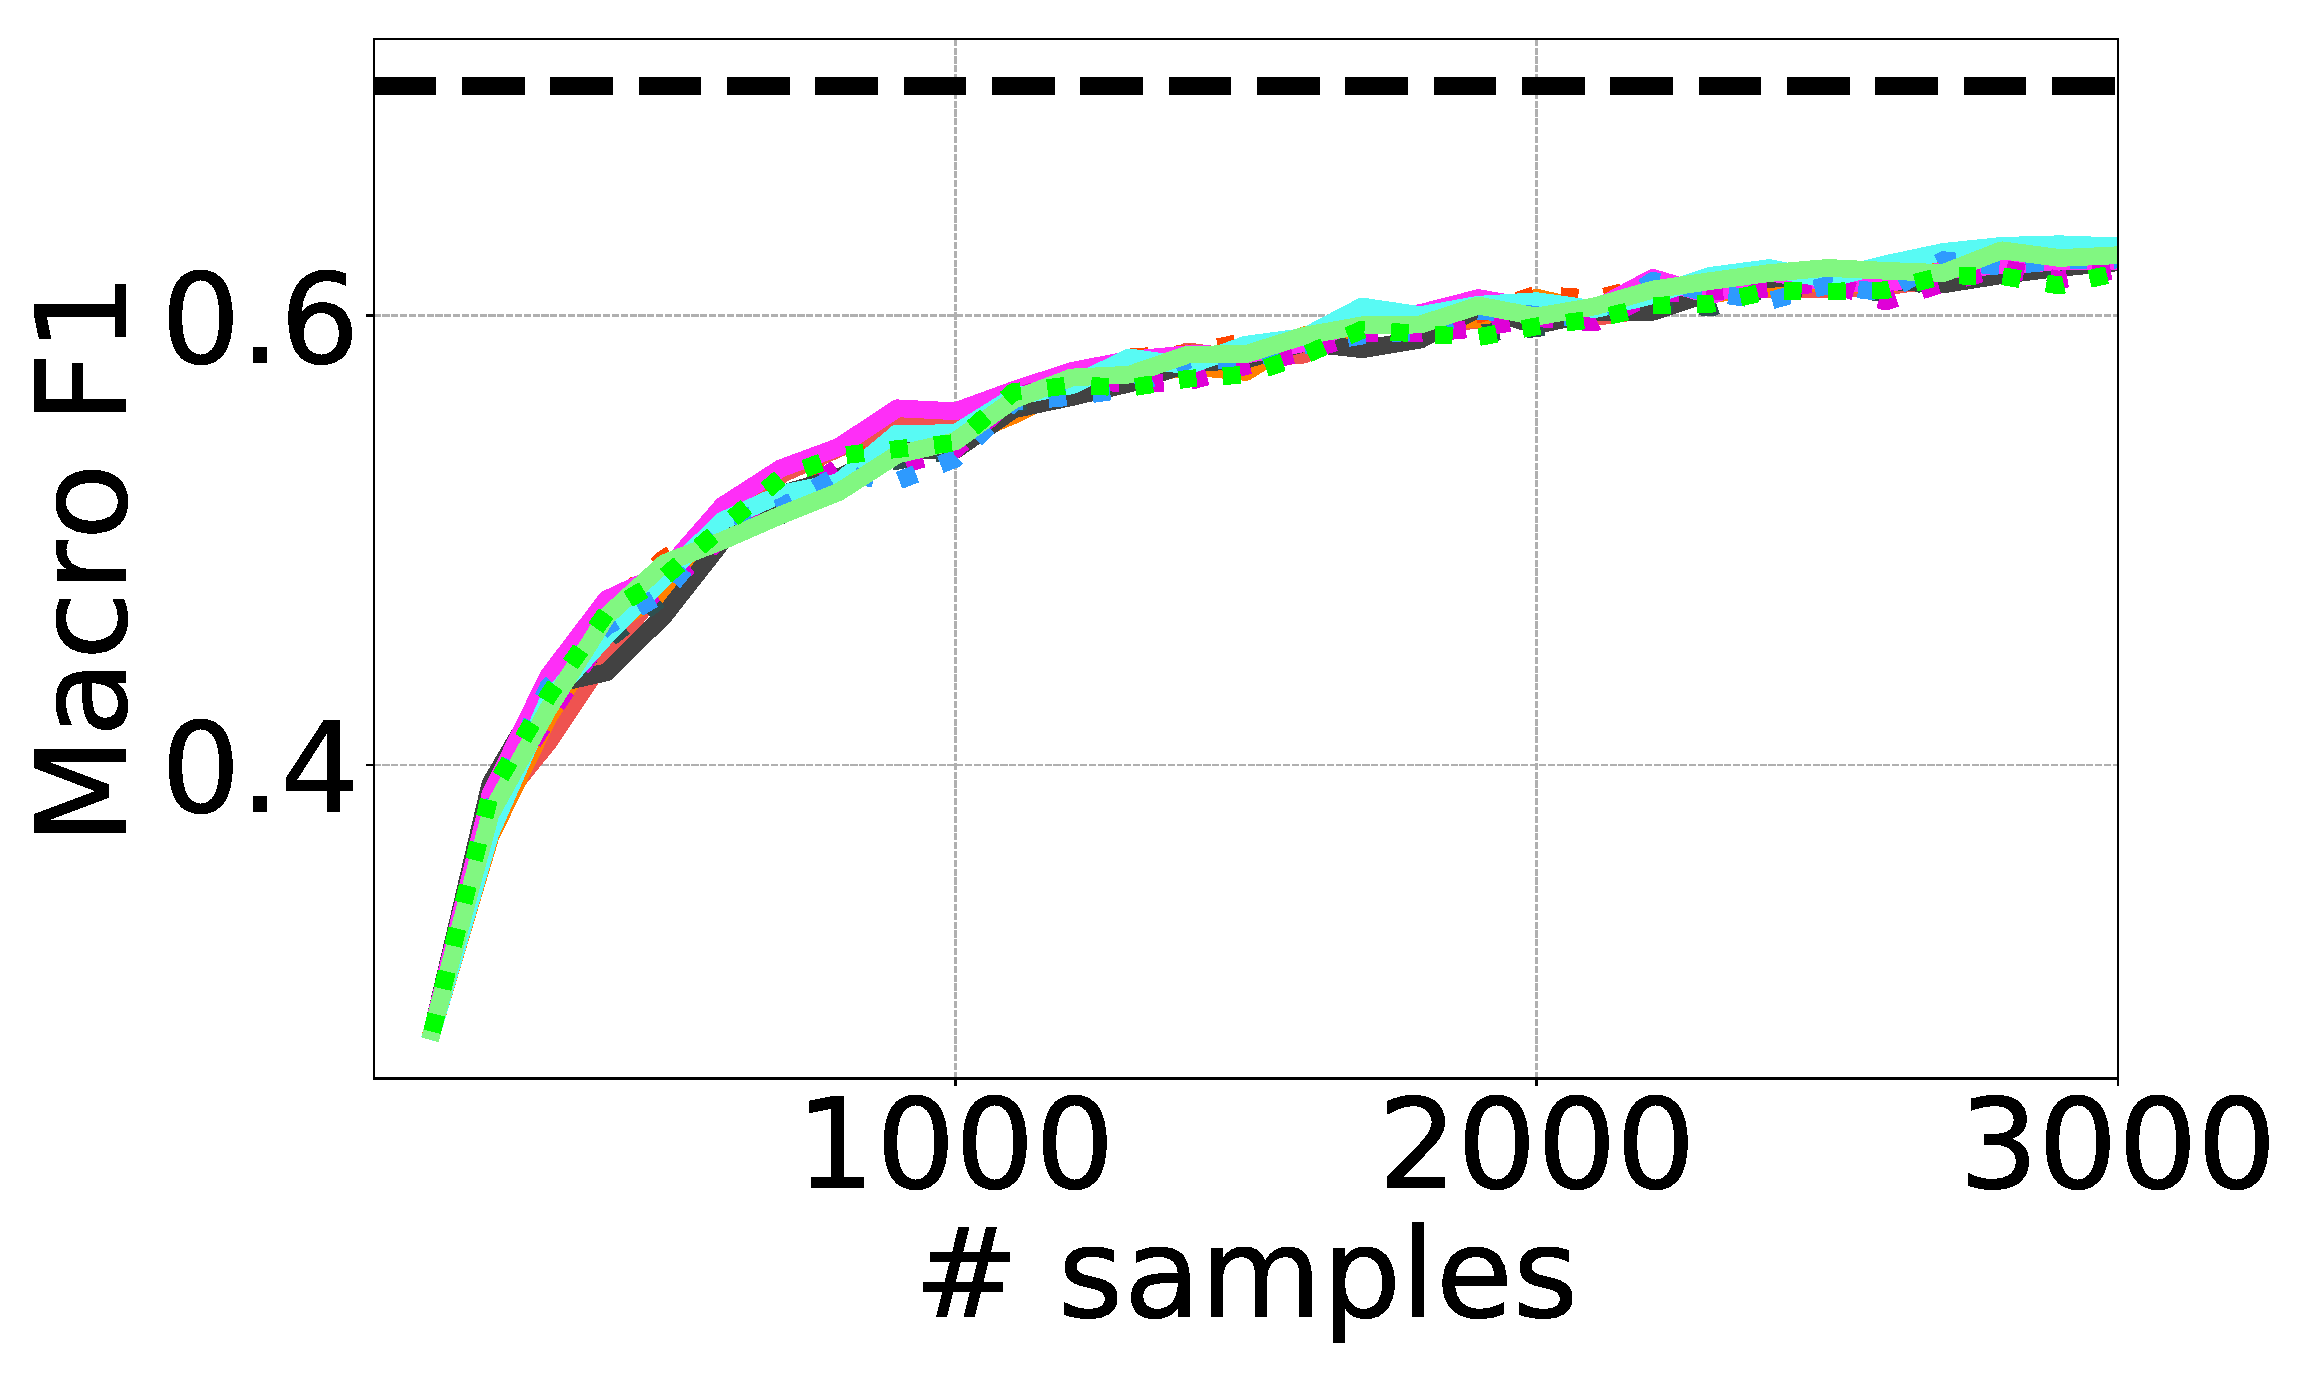
\includegraphics[width=0.23\textwidth]{res/lstm_pytorch_Biomedical_tokenized_acc_all.eps}}
		\subfloat[SearchSnippets]{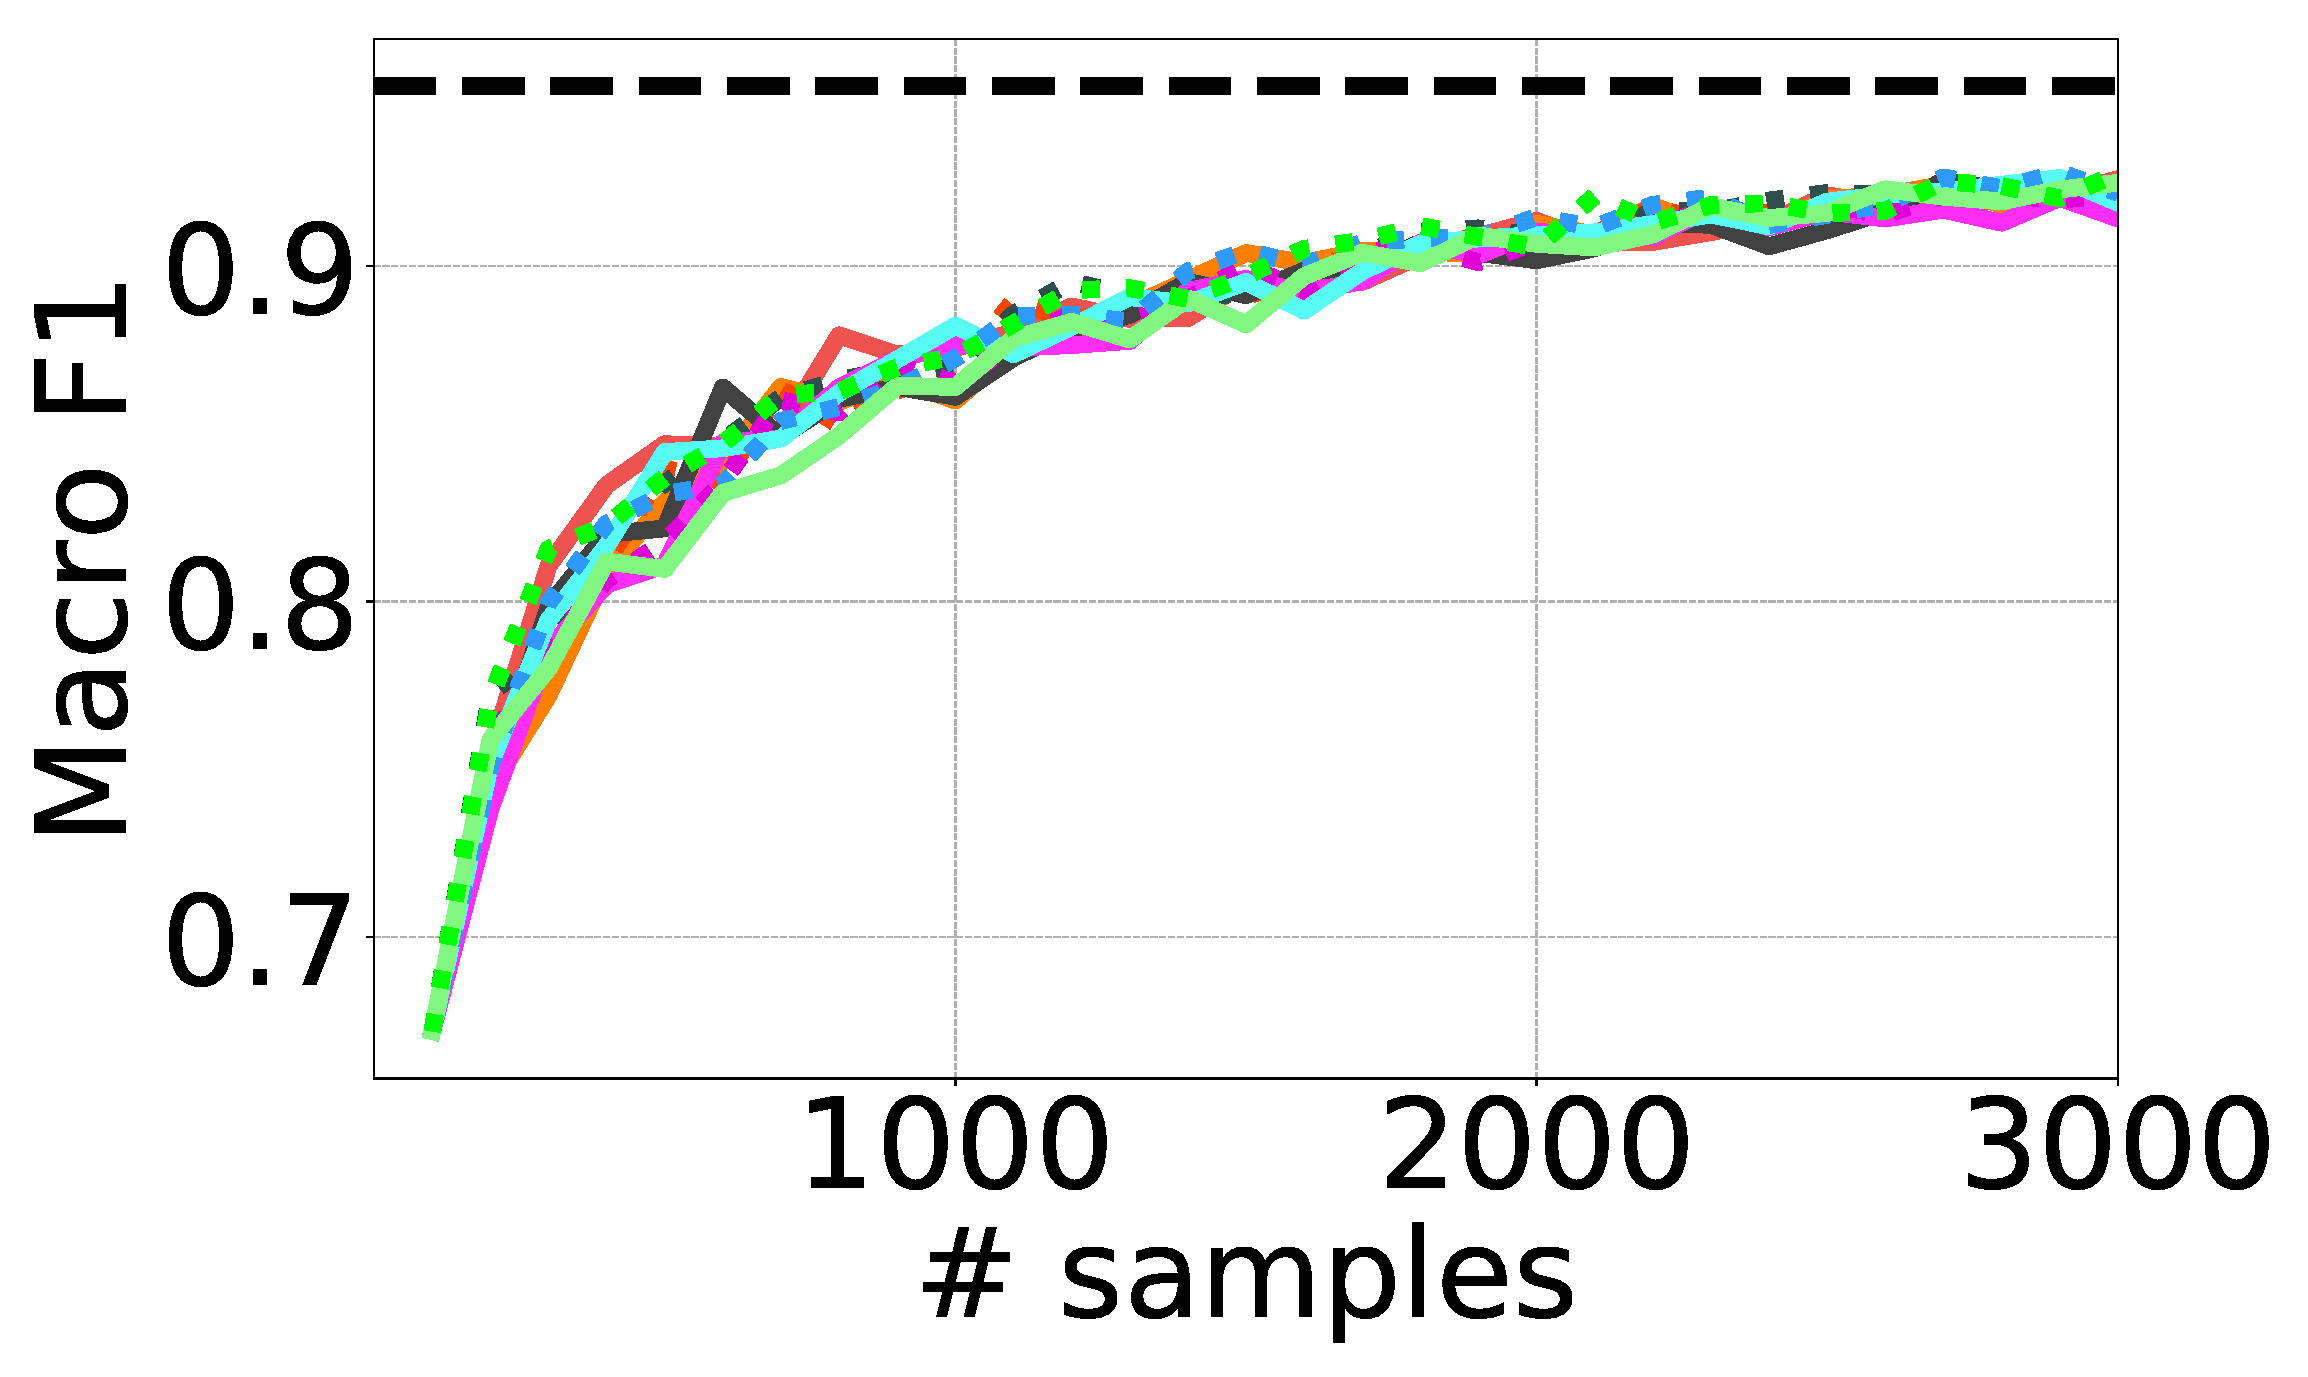
\includegraphics[width=0.23\textwidth]{res/lstm_pytorch_SearchSnippets_tokenized_acc_all.eps}}
	\end{center}
	\noindent
	\begin{center}
		\subfloat[Emoji]{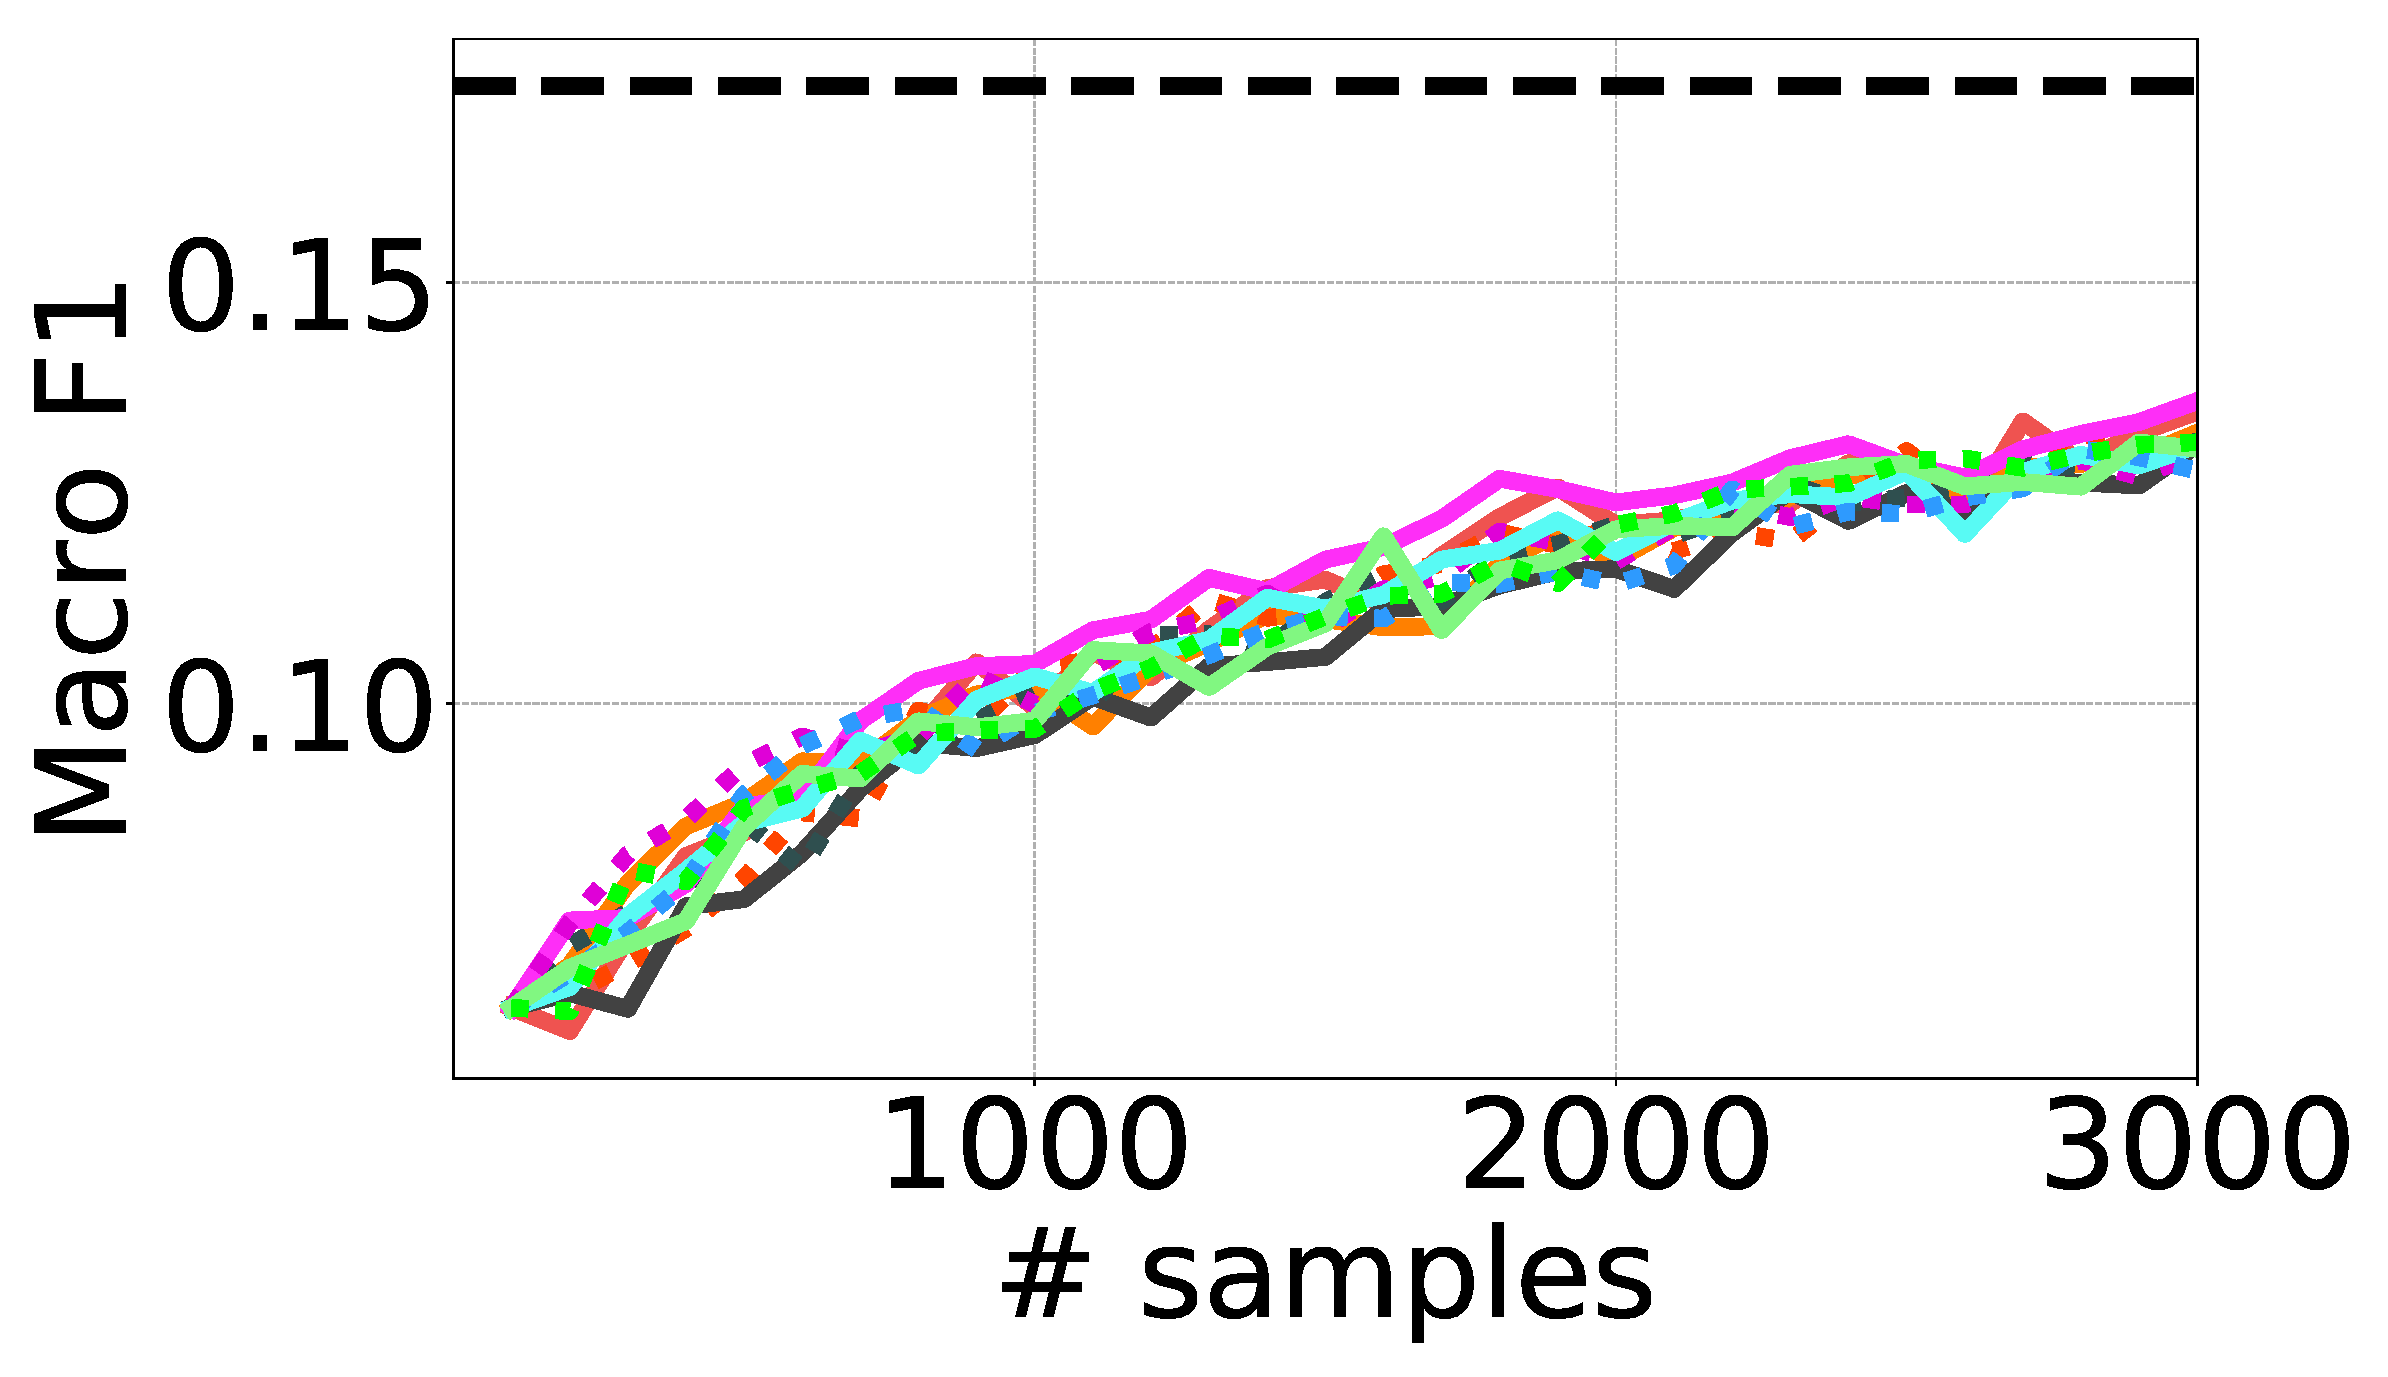
\includegraphics[width=0.23\textwidth]{res/lstm_pytorch_emoji_tokenized_acc_all.eps}} 
		\subfloat[TNEWS]{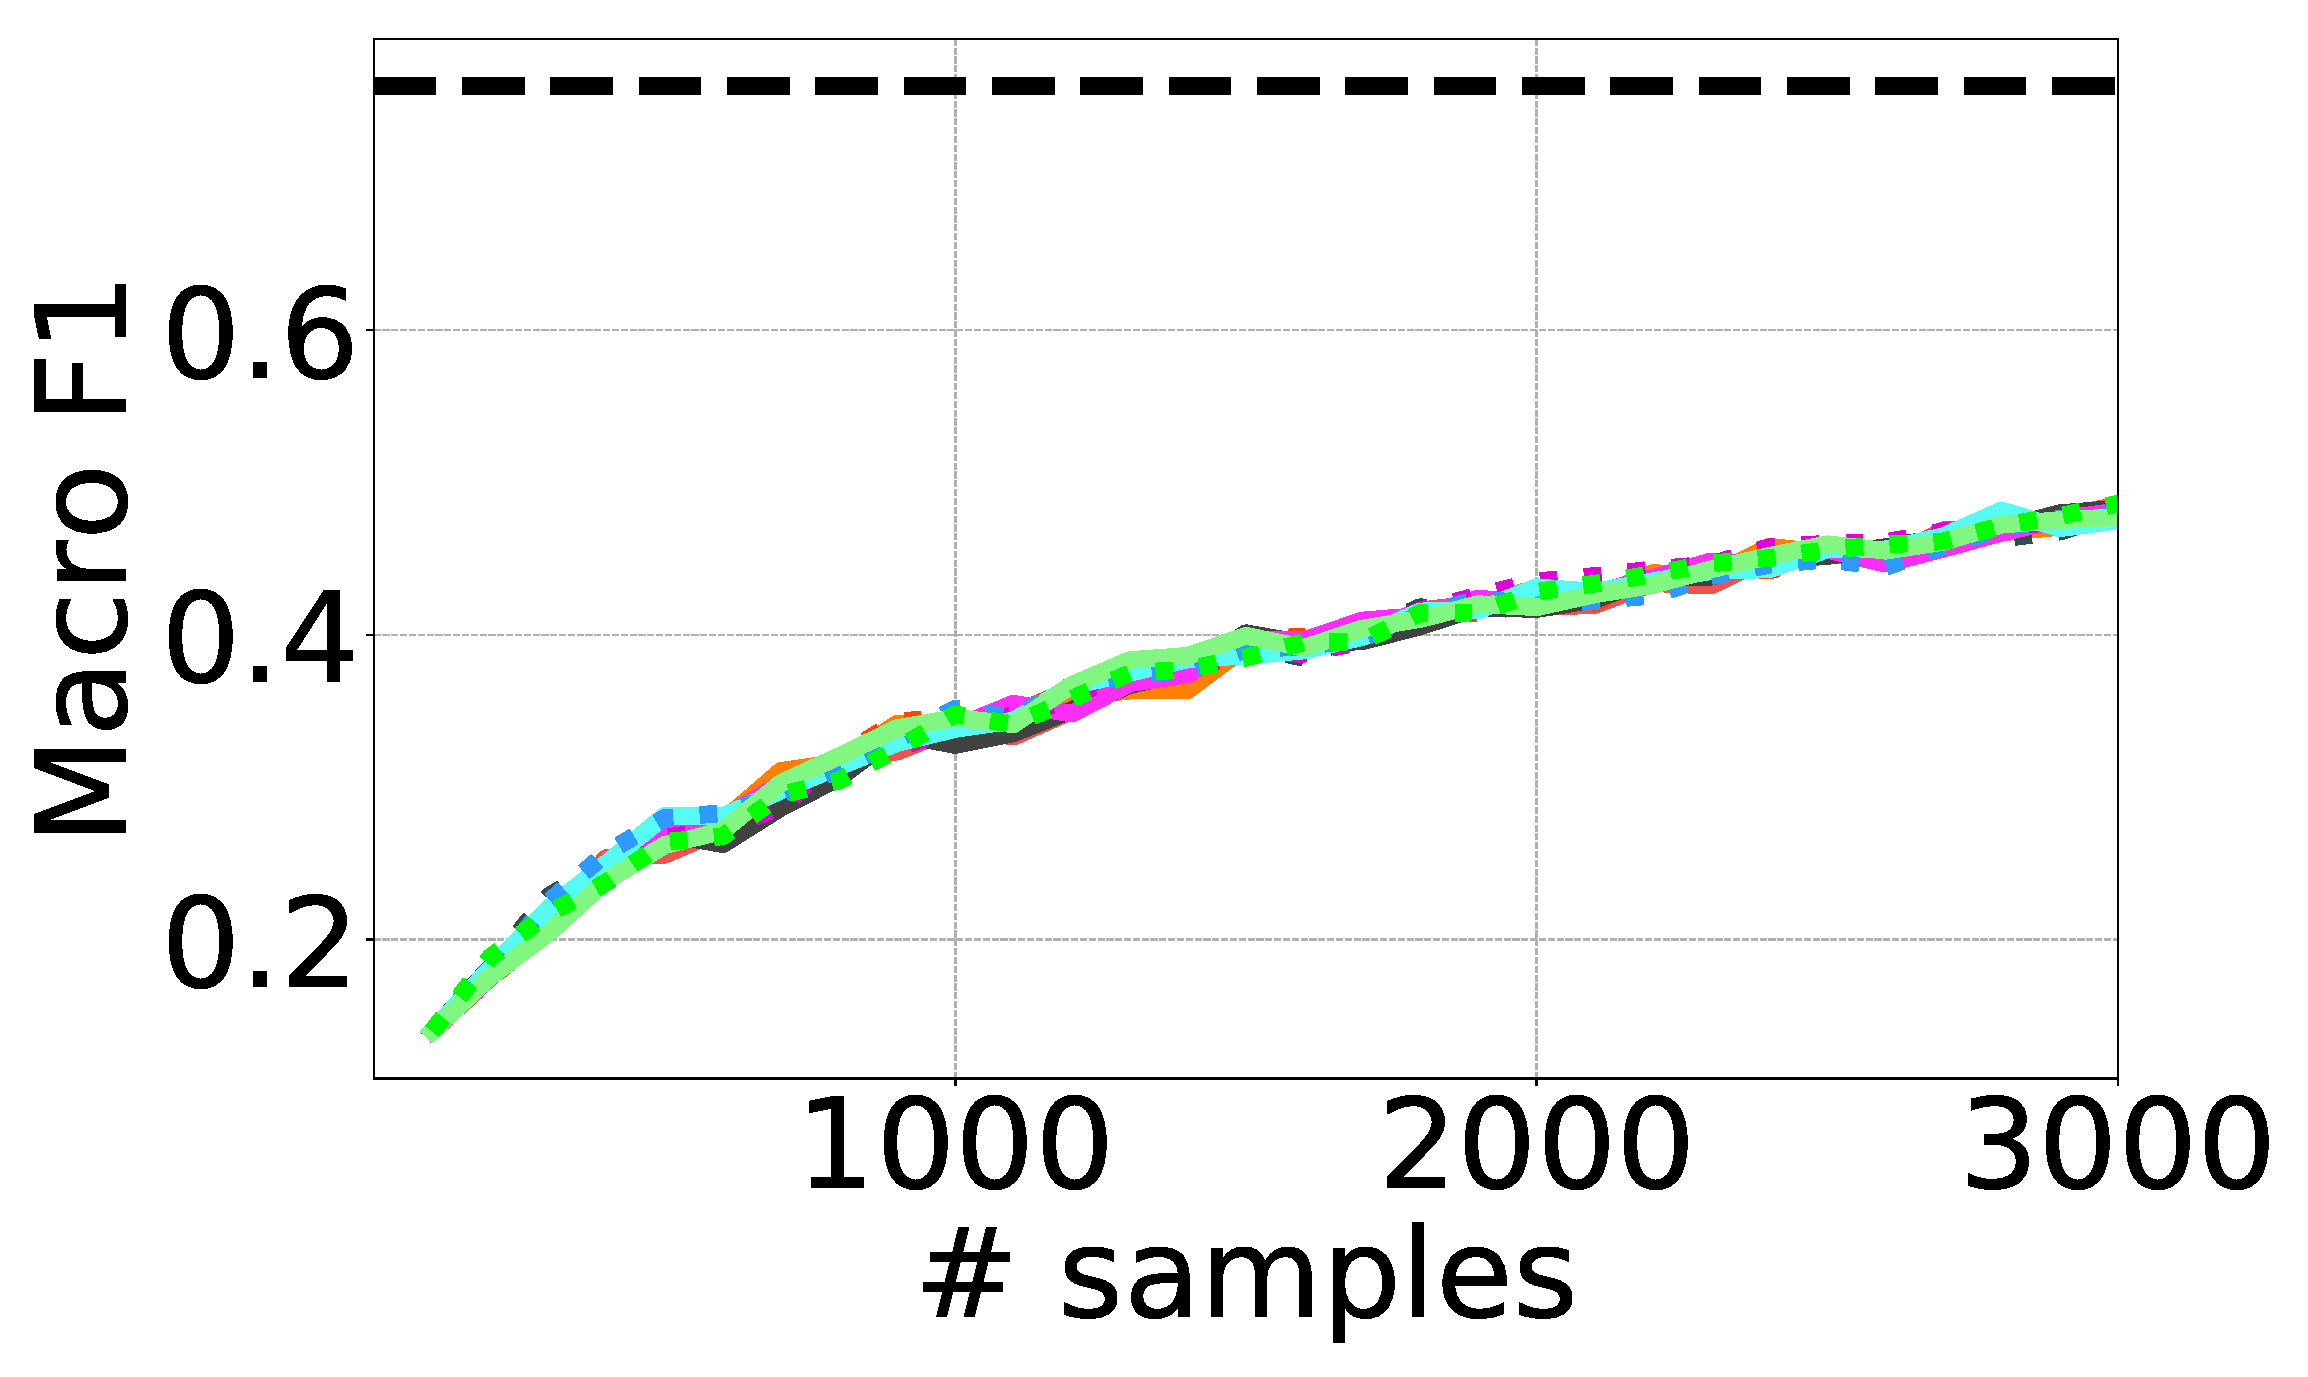
\includegraphics[width=0.23\textwidth]{res/lstm_pytorch_tnews_tokenized_acc_all.eps}} 
		\subfloat[GCS]{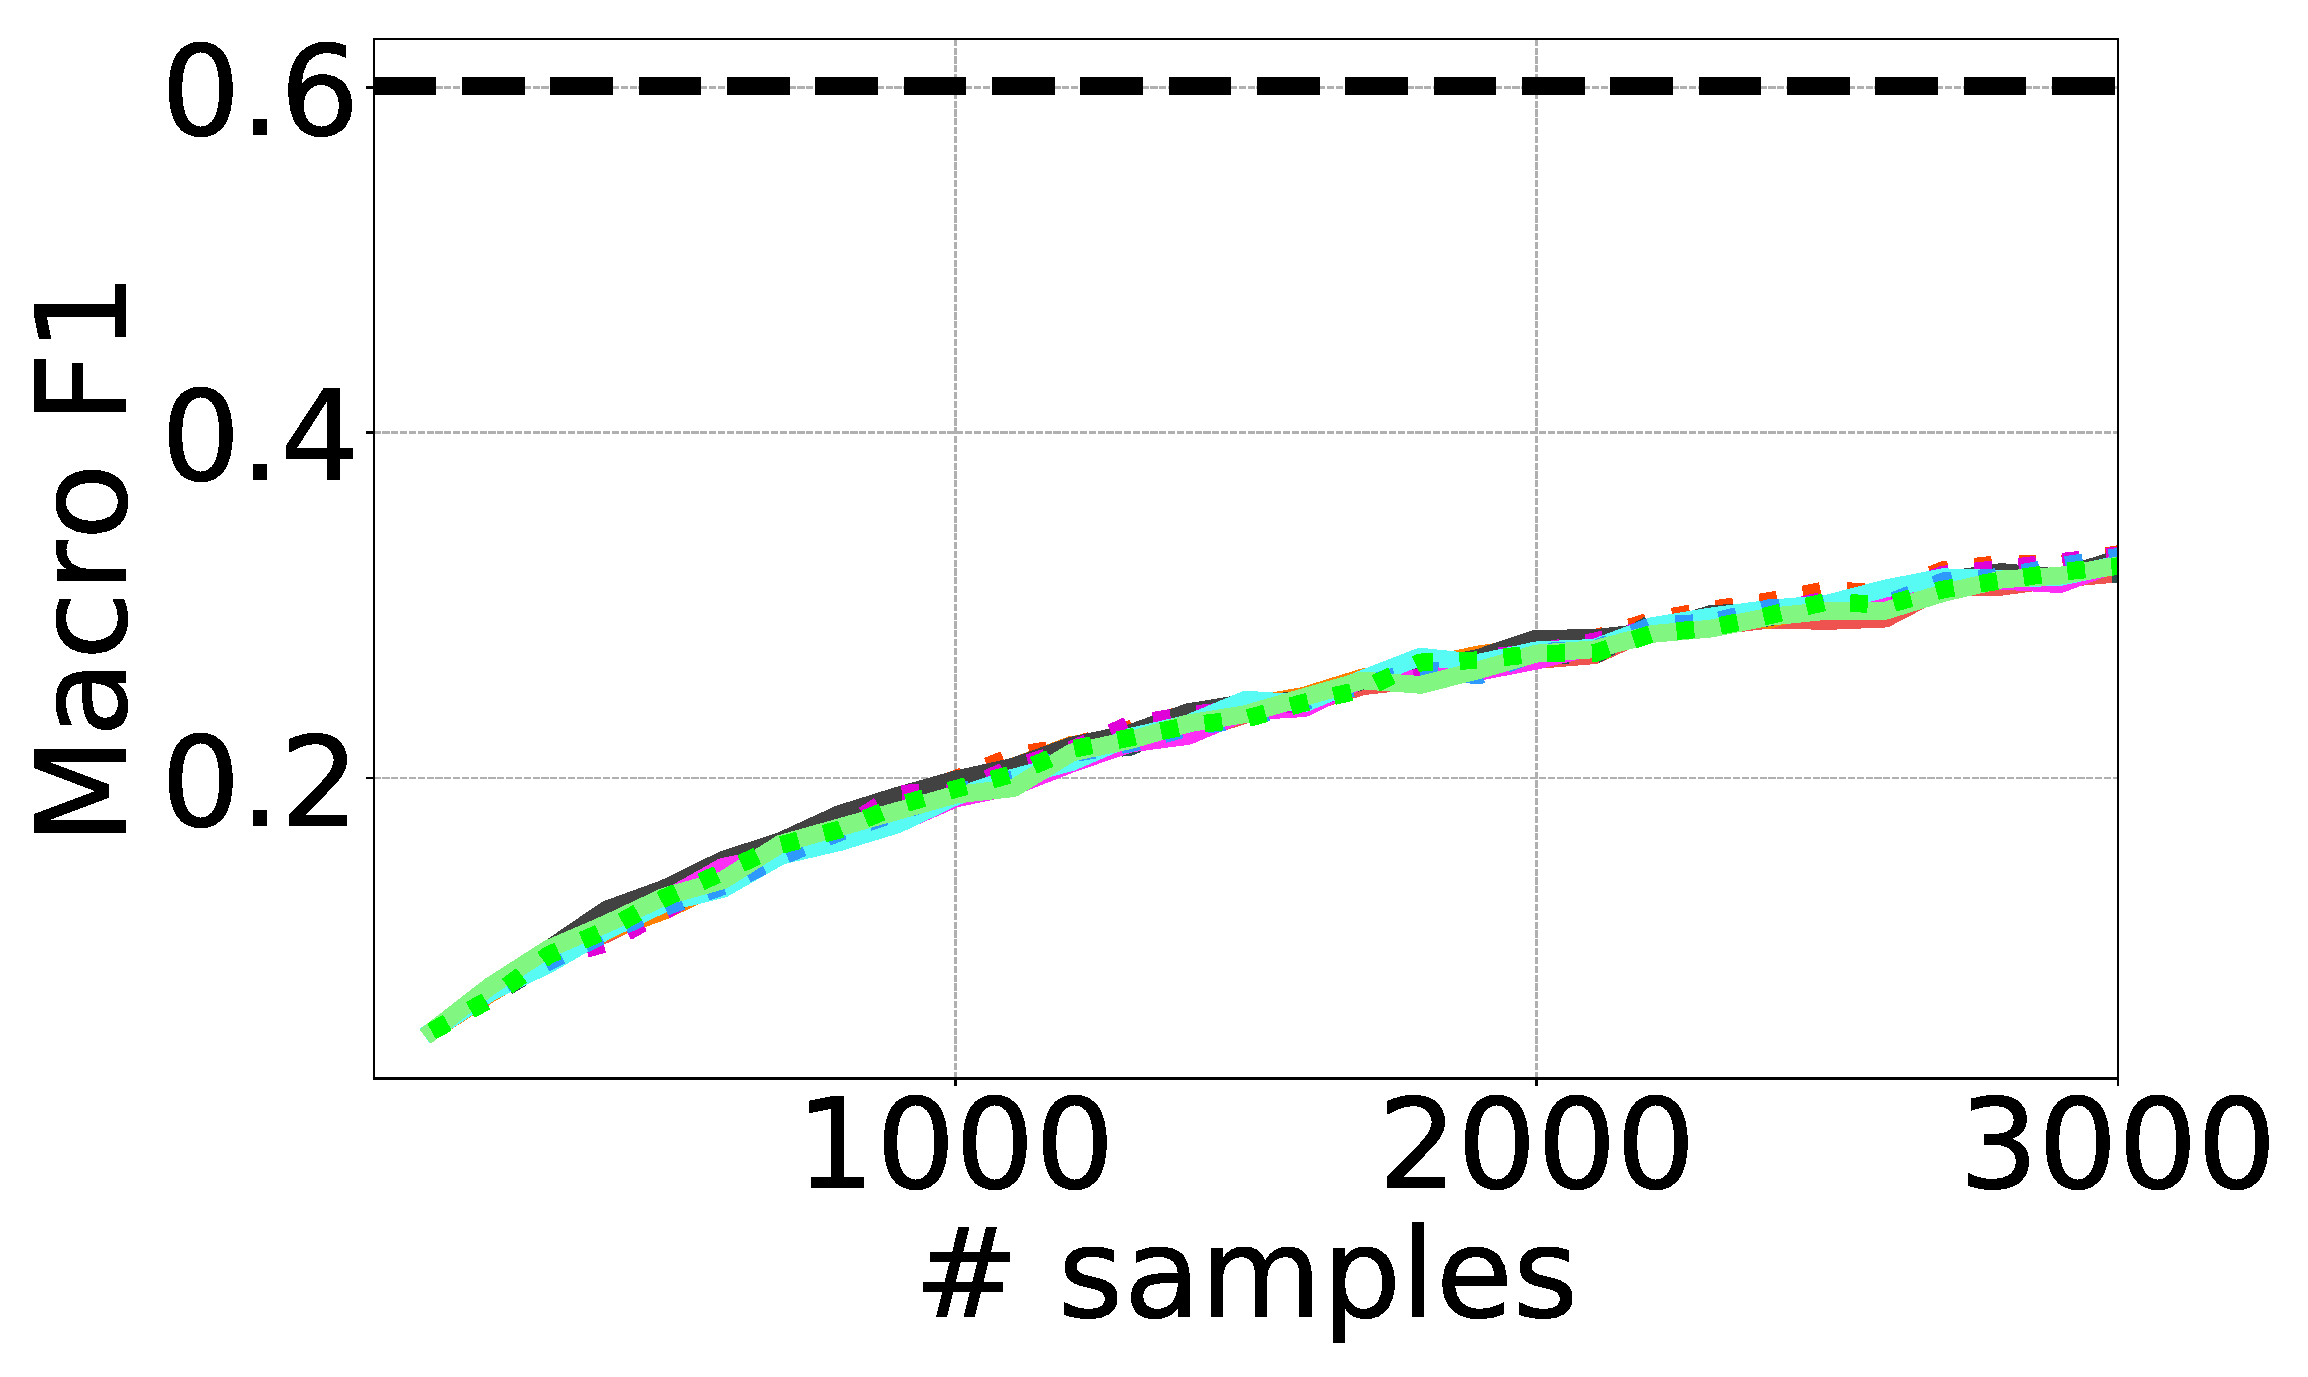
\includegraphics[width=0.23\textwidth]{res/lstm_pytorch_yanjing_tokenized_acc_all.eps}}
		\subfloat[Book]{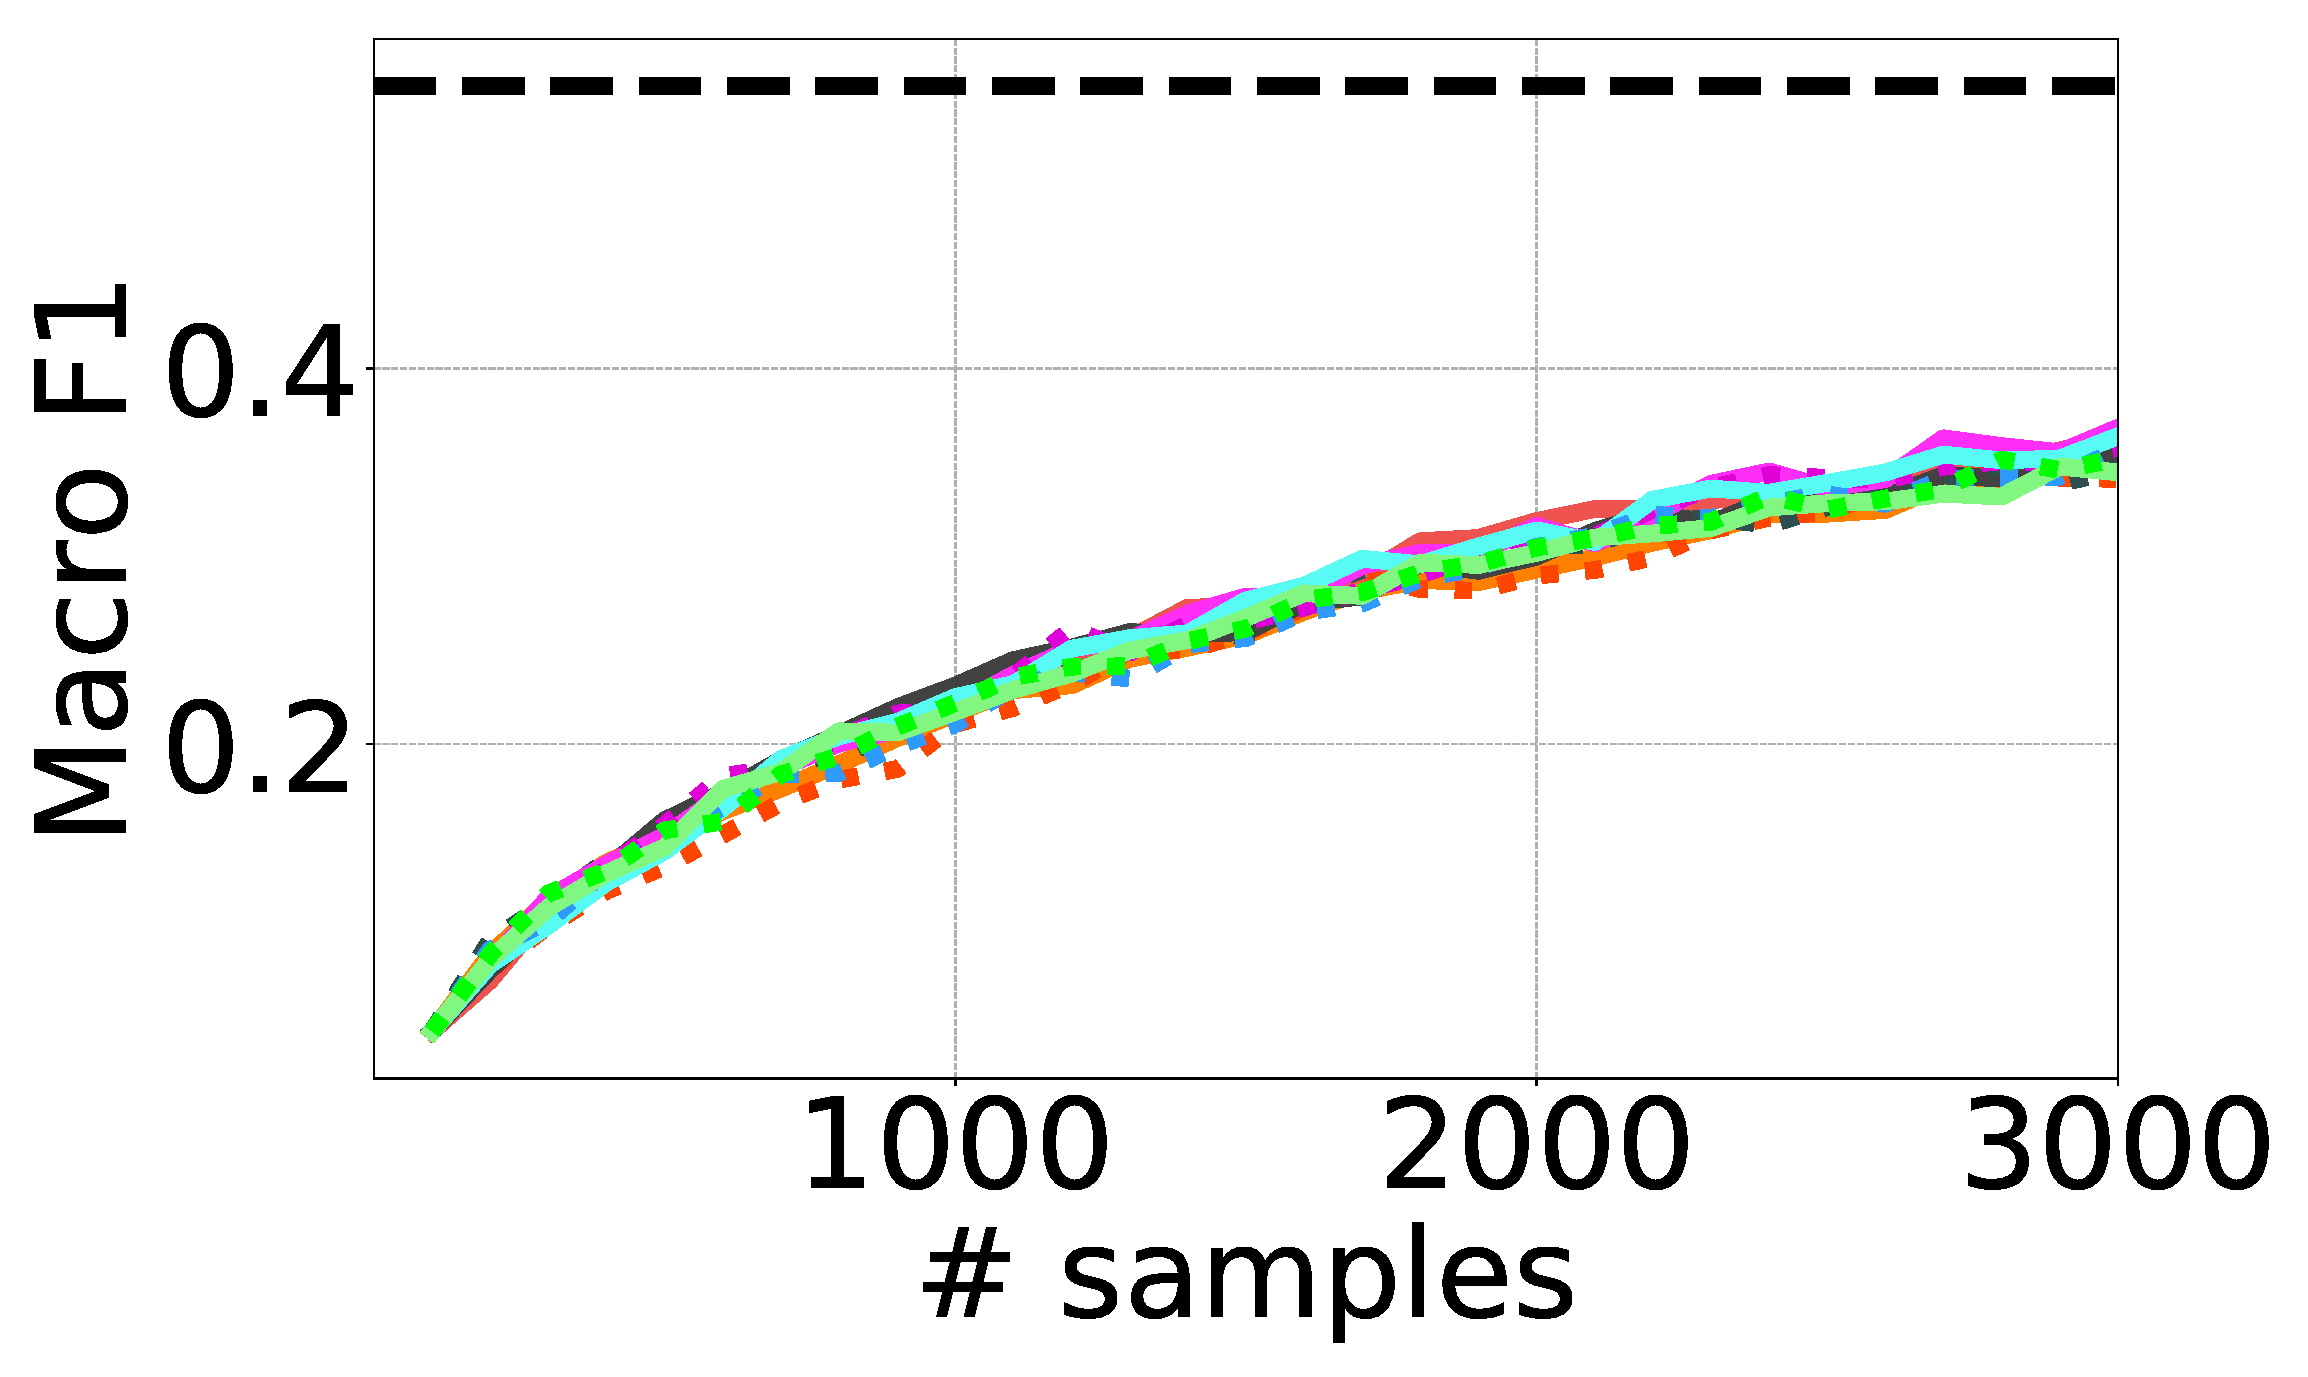
\includegraphics[width=0.23\textwidth]{res/lstm_pytorch_book_tokenized_acc_all.eps}}
	\end{center}
	\caption{Macro F1 curve of AL approaches on 8 datasets using LSTM.}
	\label{fig:acc_all_lstm}
\end{figure*}

\begin{figure*}[th!]%[!hbt]
	\noindent
	\begin{center}
		\subfloat[Reuters]{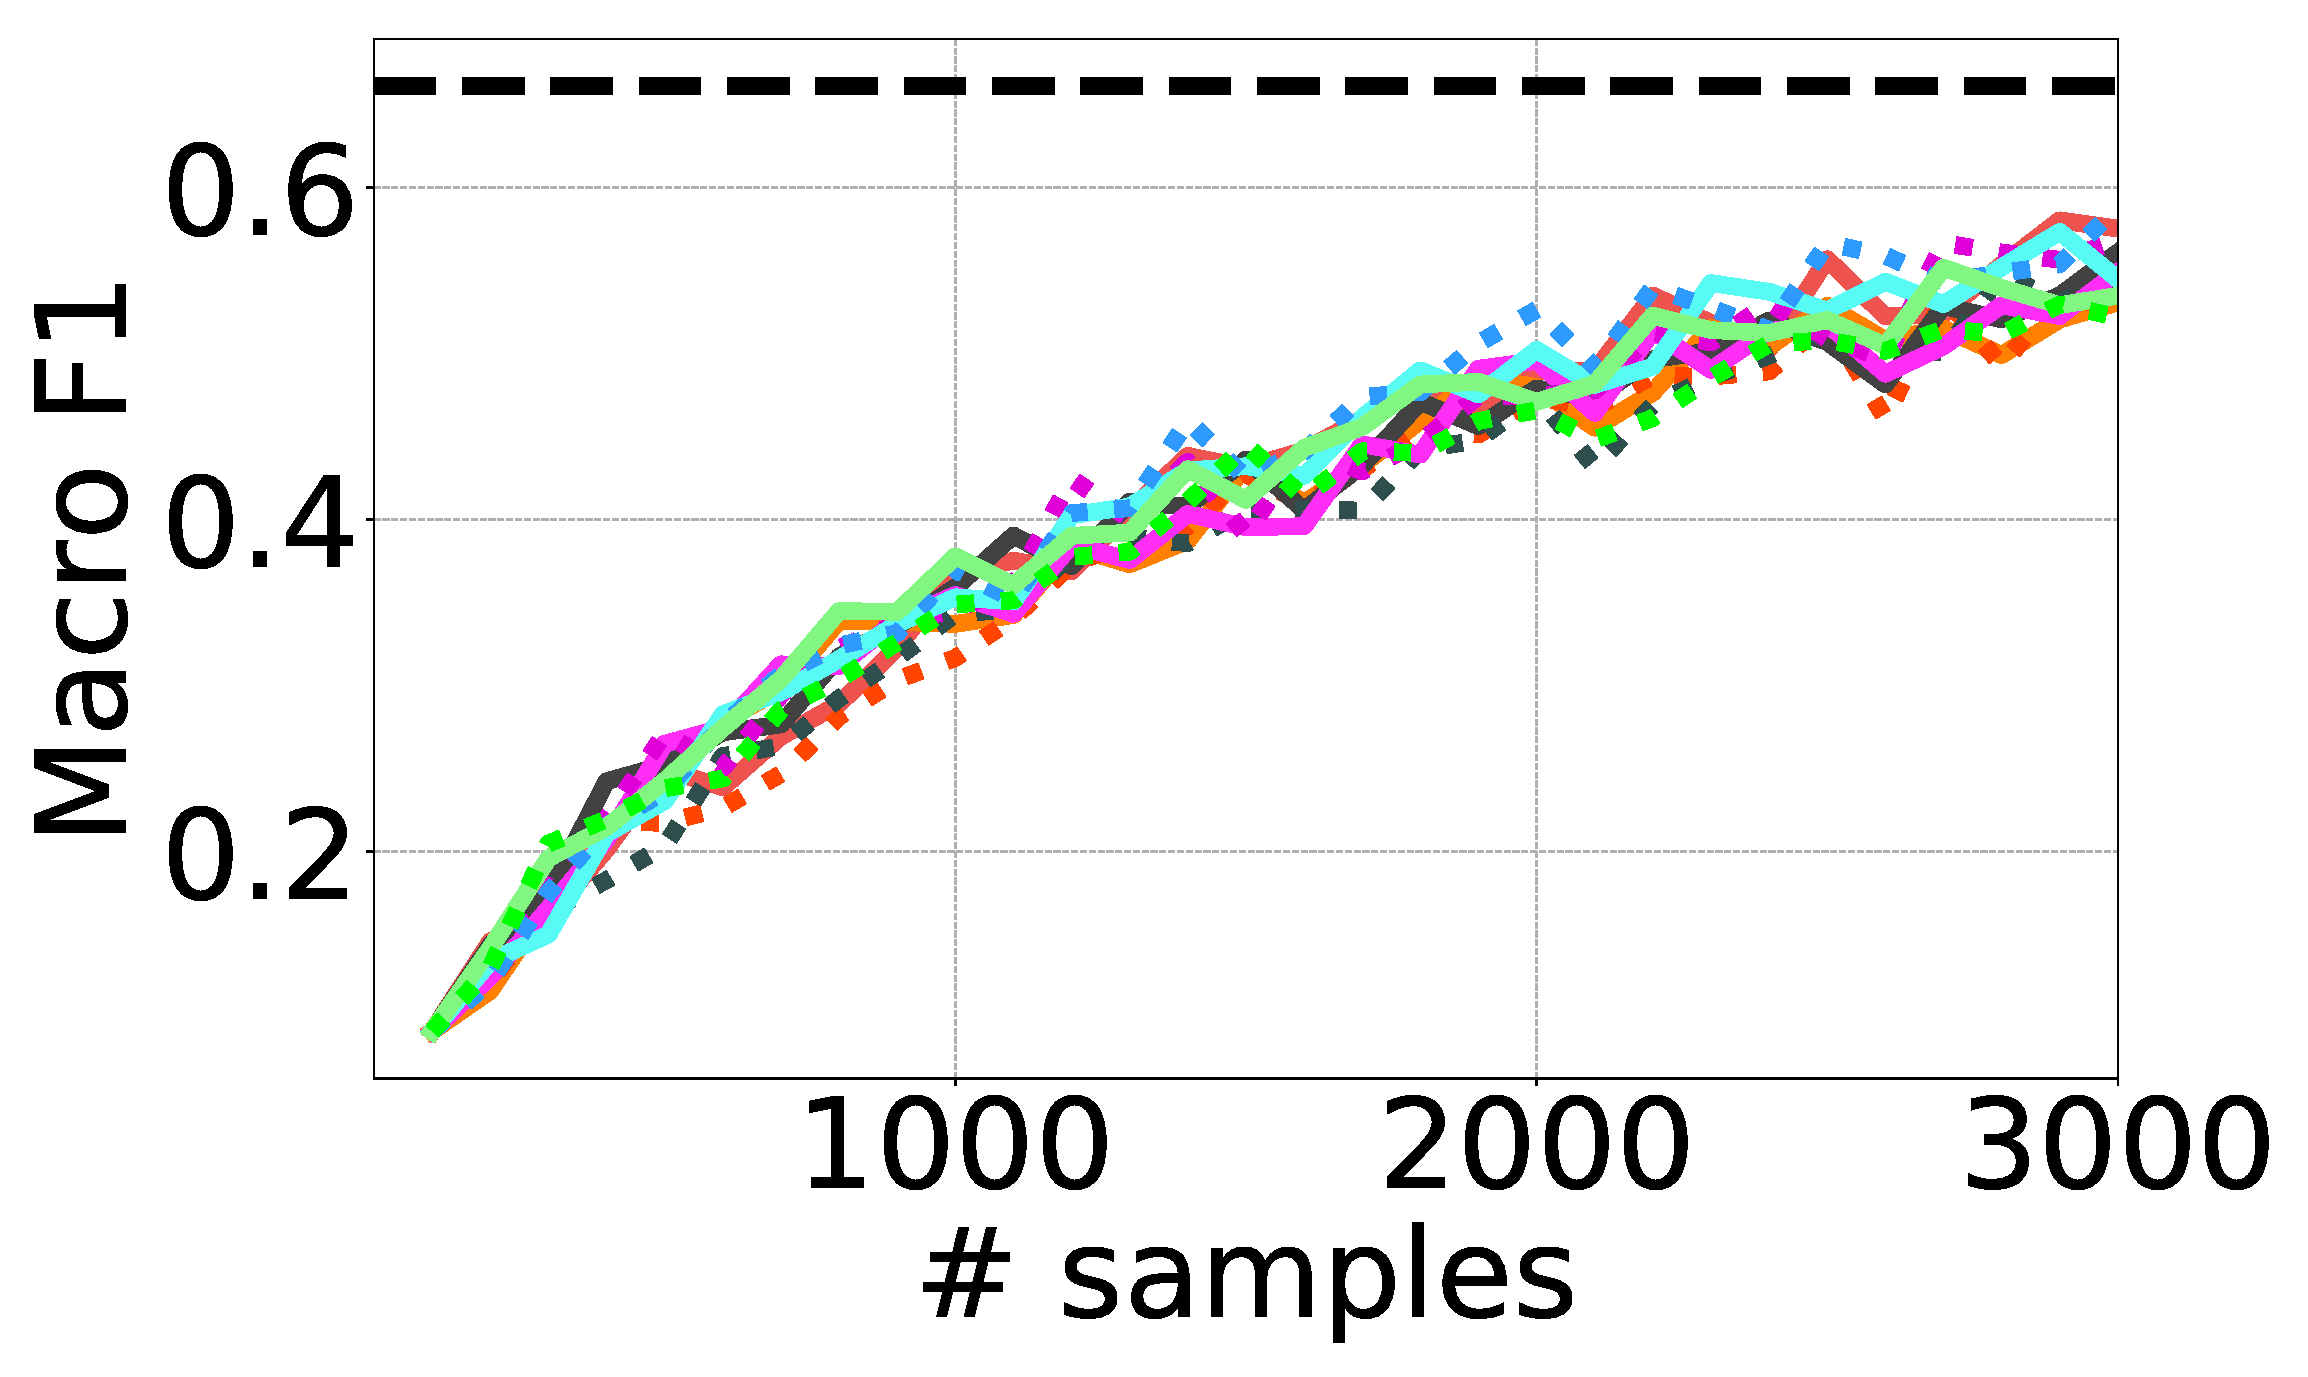
\includegraphics[width=0.23\textwidth]{res/cnn_pytorch_reuters_new_acc_all.eps}}
		\subfloat[HuffPost]{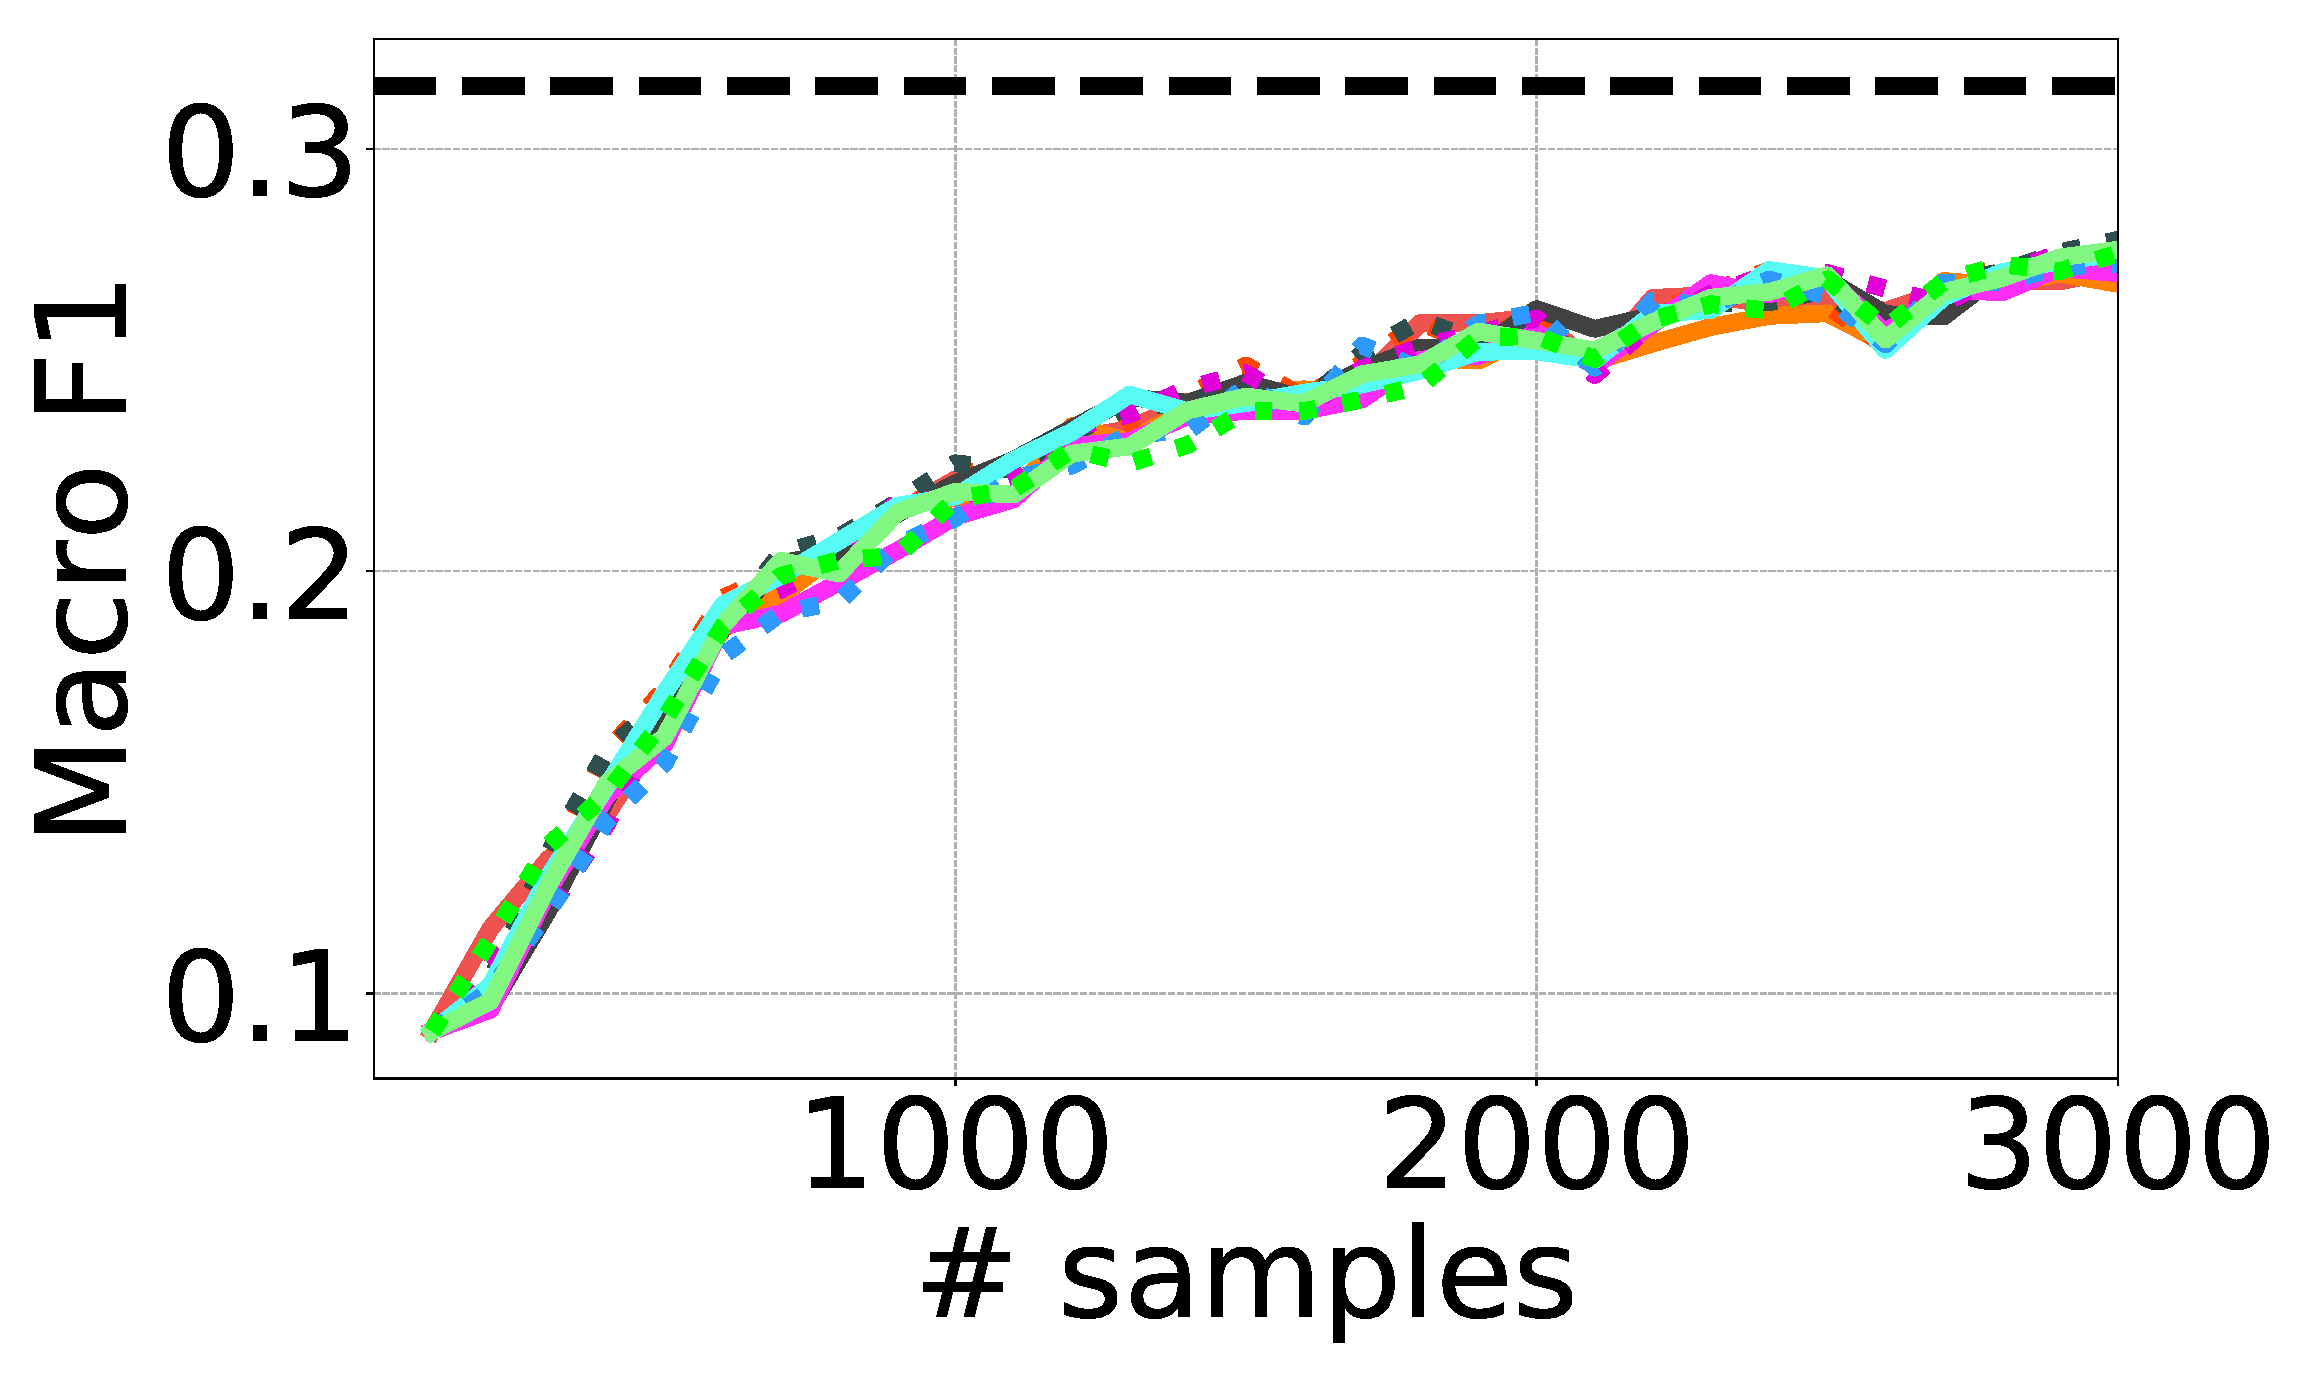
\includegraphics[width=0.23\textwidth]{res/cnn_pytorch_news_reshuffle_tokenized_acc_all.eps}}
		\subfloat[Biomedical]{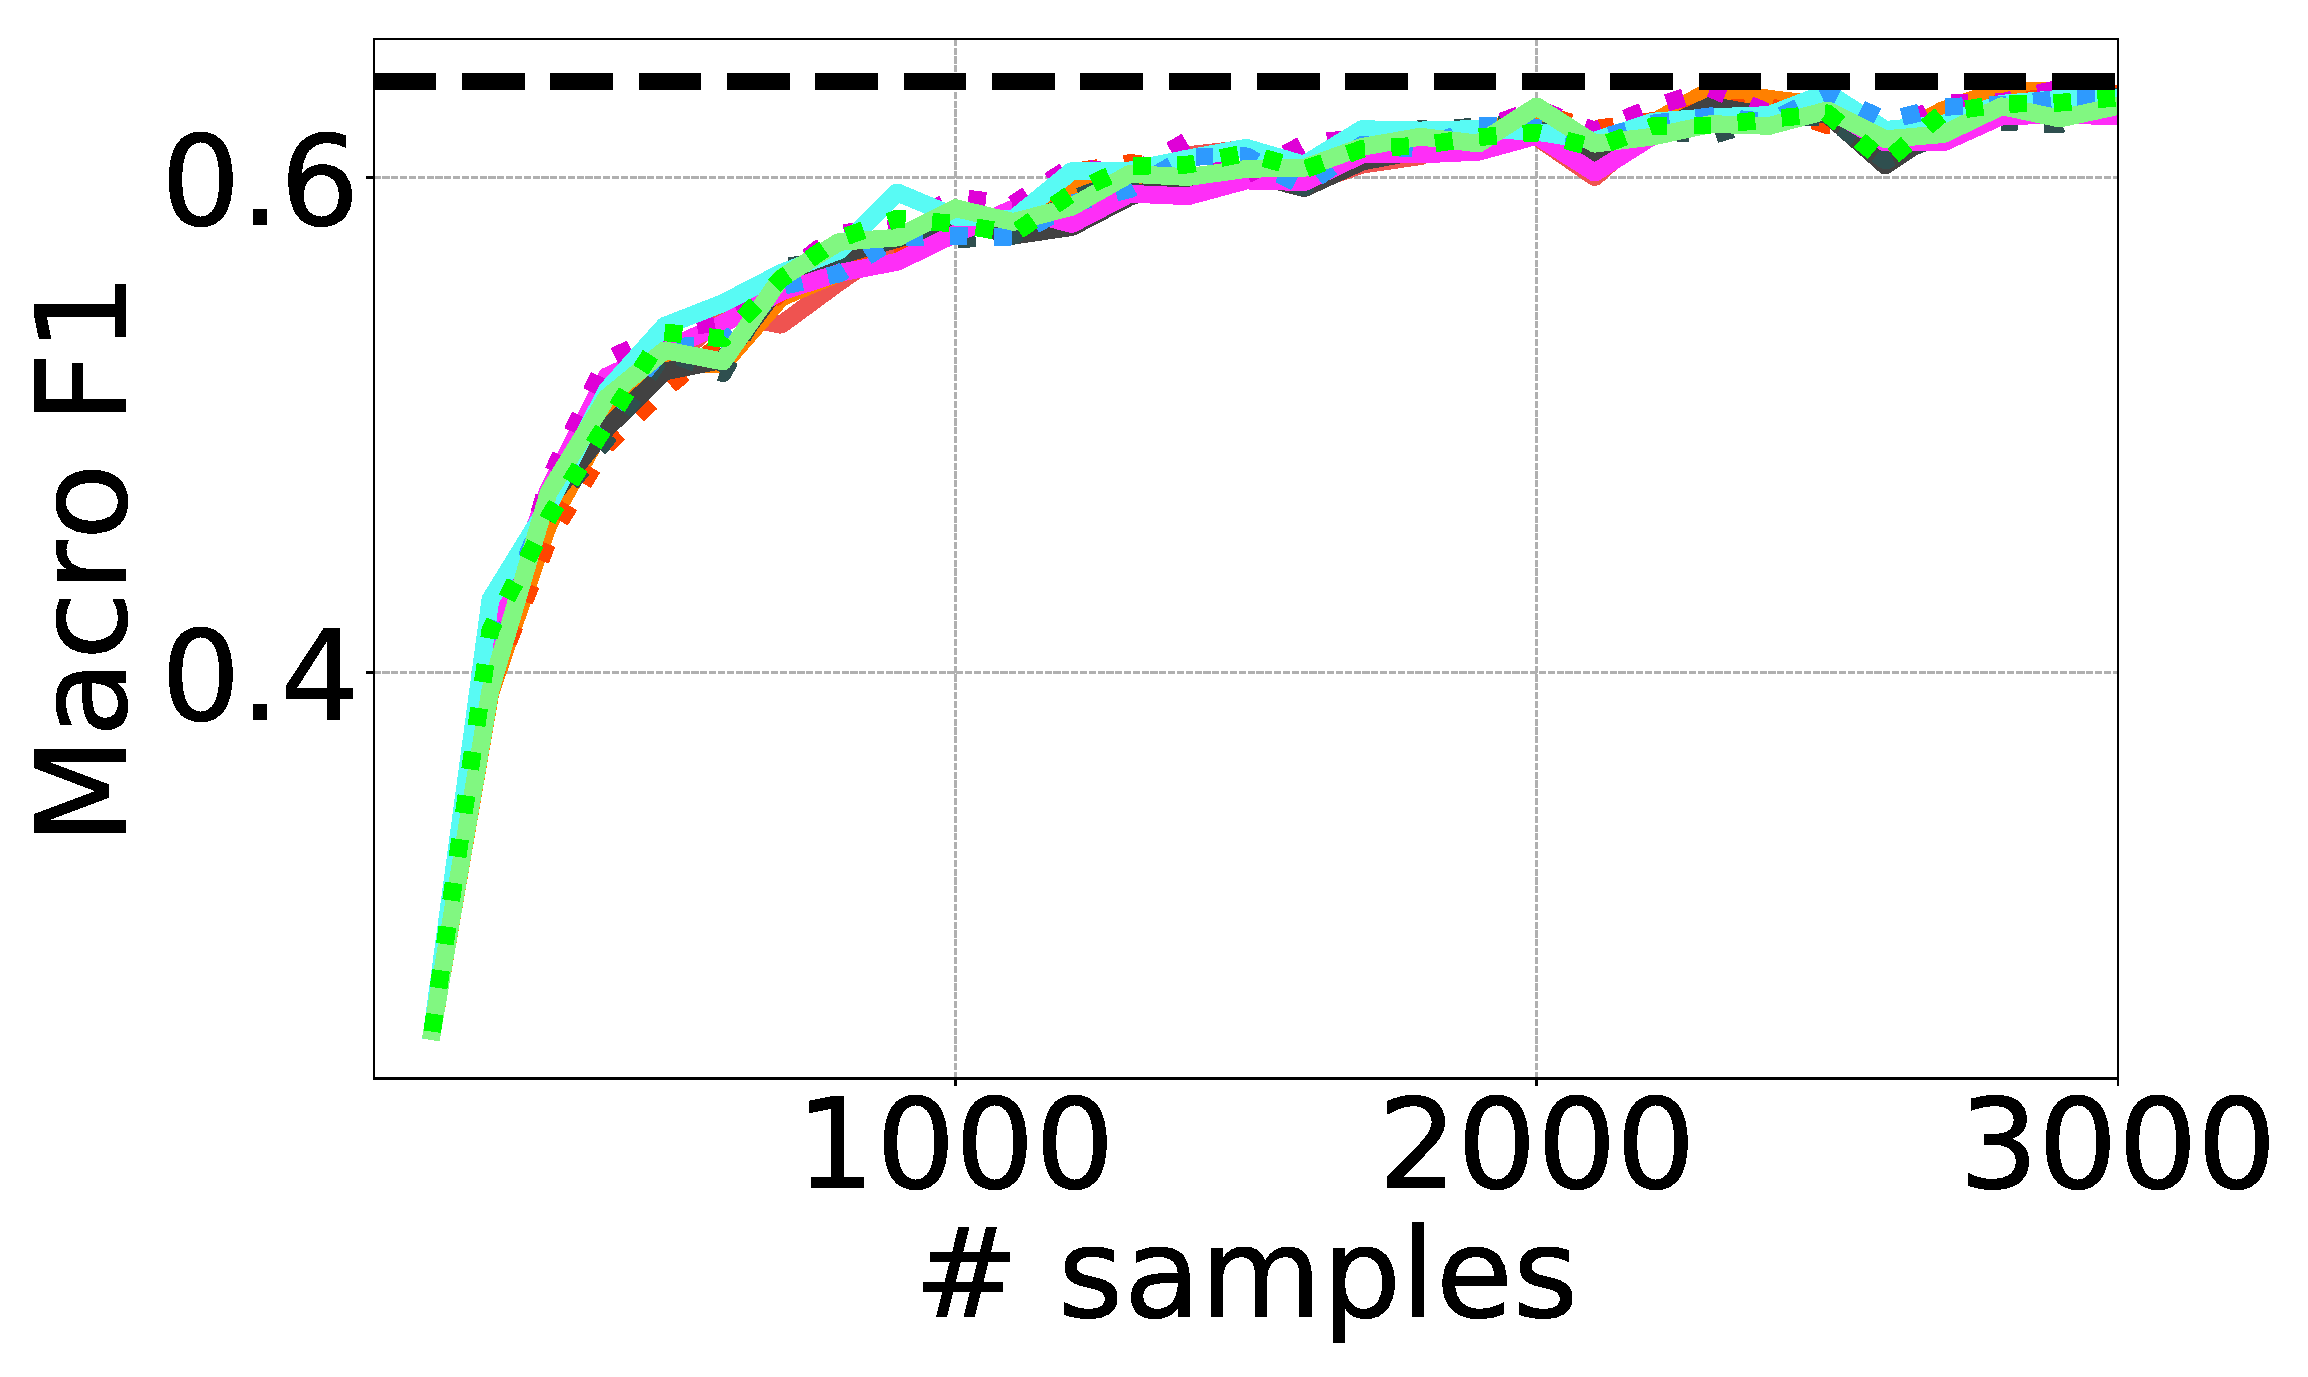
\includegraphics[width=0.23\textwidth]{res/cnn_pytorch_Biomedical_tokenized_acc_all.eps}}
		\subfloat[SearchSnippets]{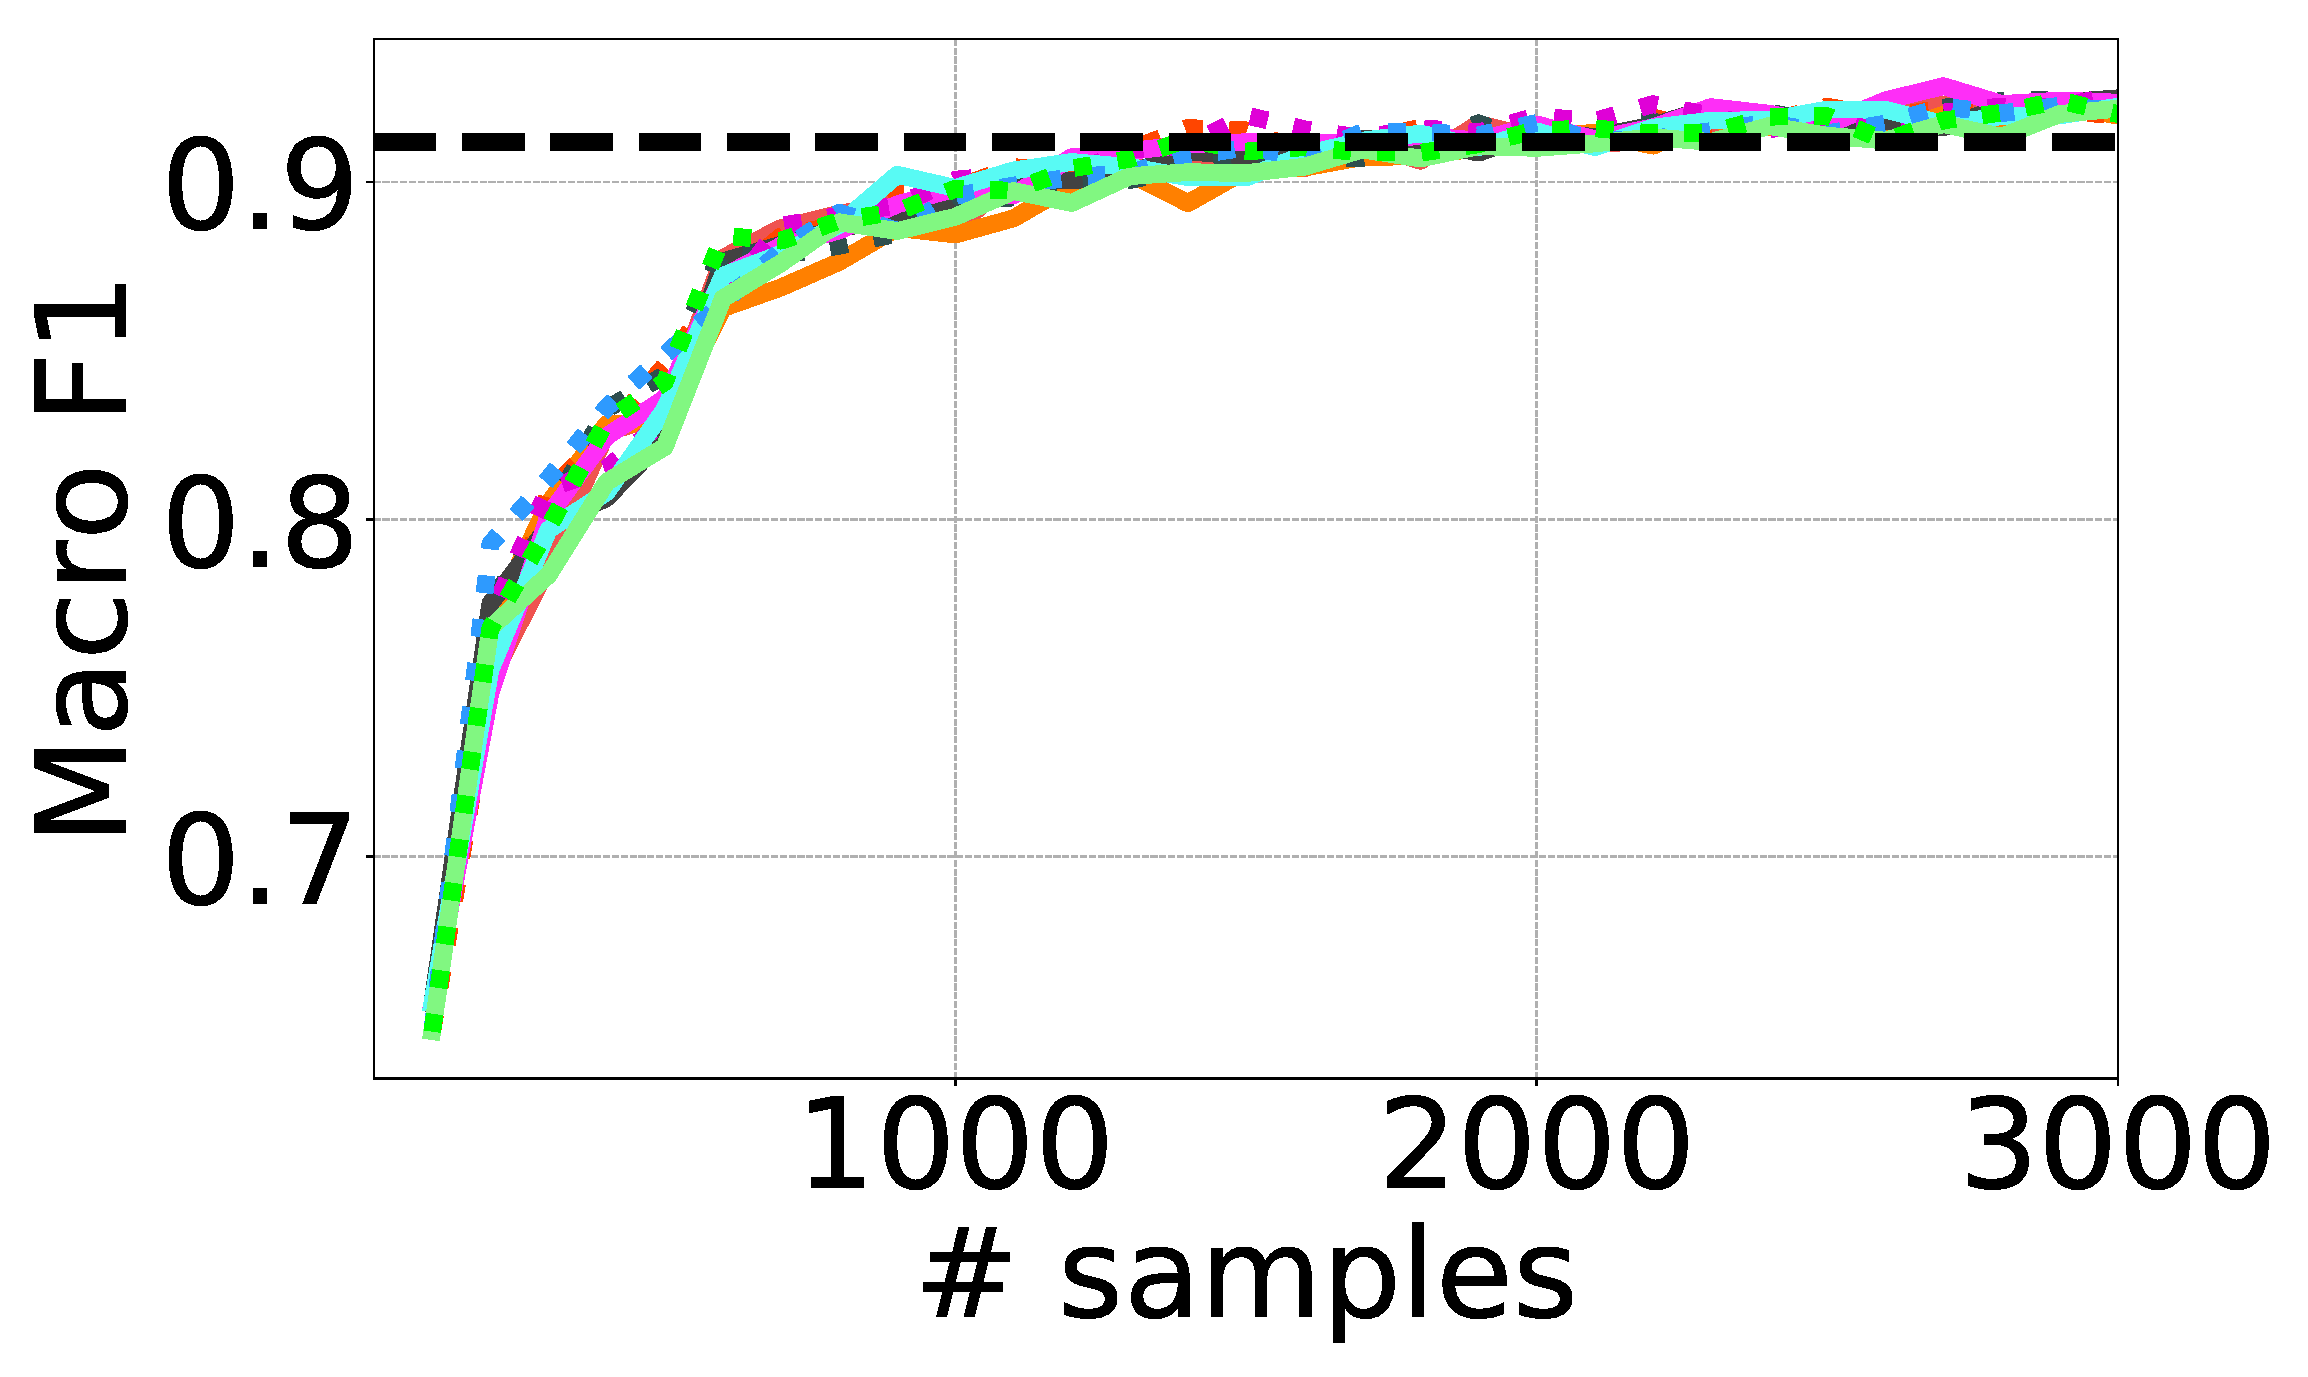
\includegraphics[width=0.23\textwidth]{res/cnn_pytorch_SearchSnippets_tokenized_acc_all.eps}}
	\end{center}

	\noindent
	\begin{center}
		\subfloat[Emoji]{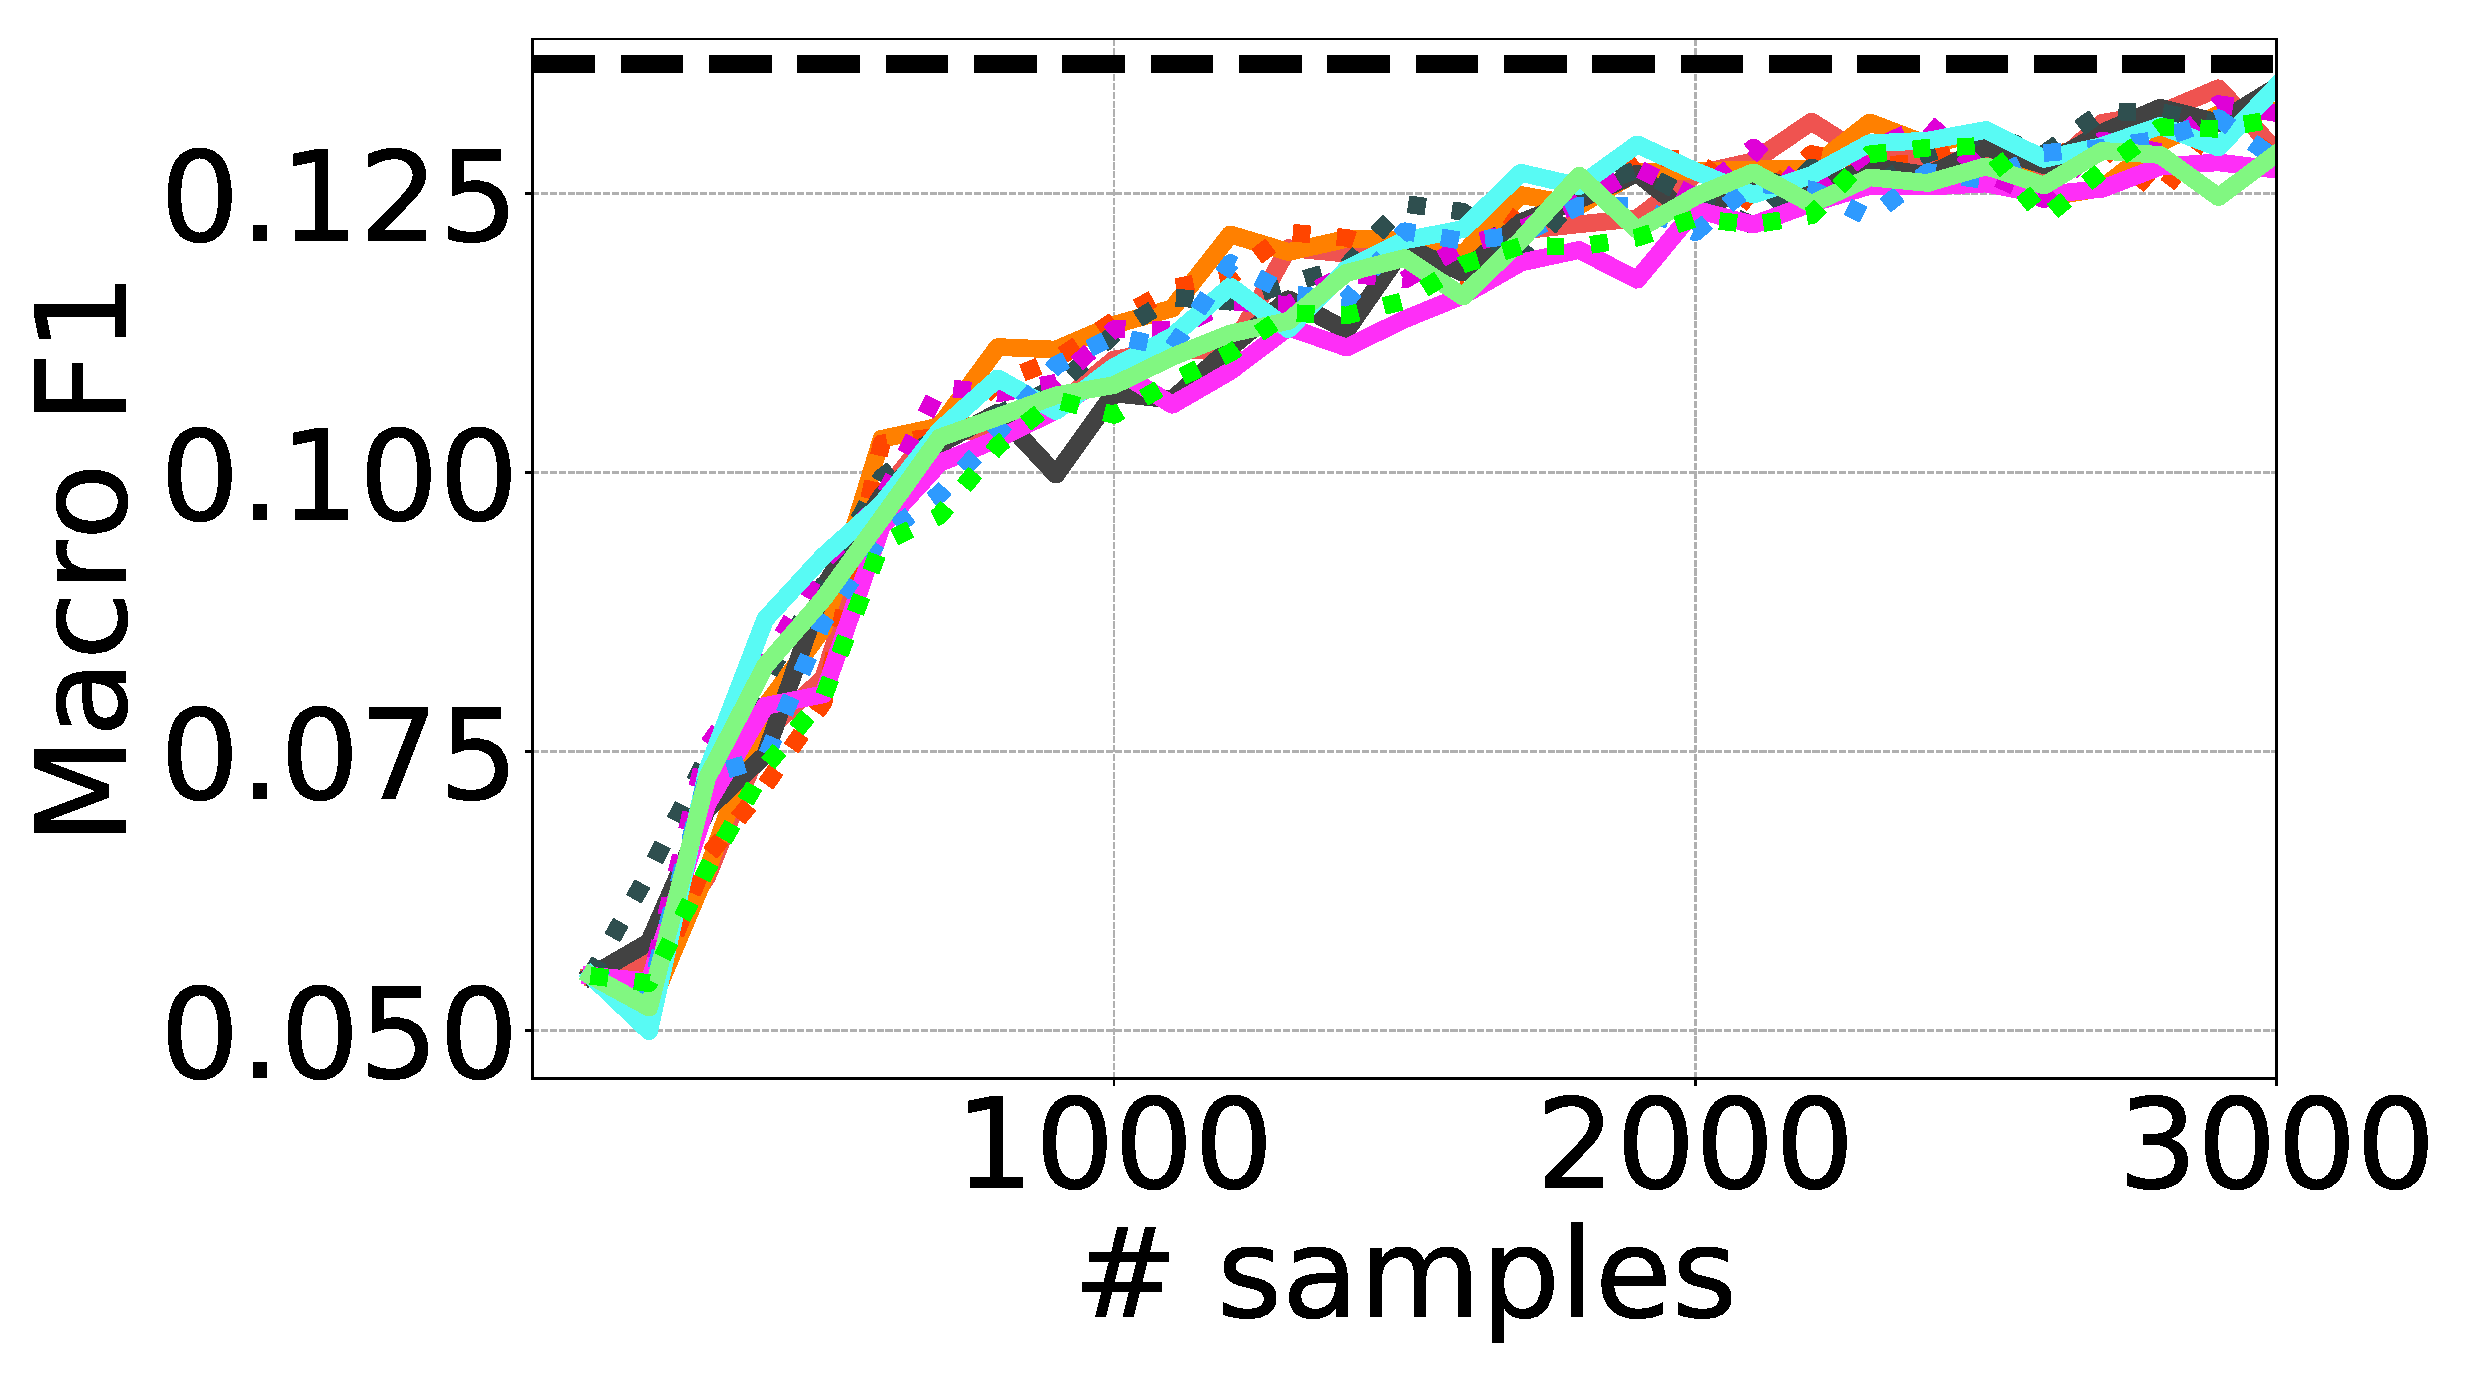
\includegraphics[width=0.23\textwidth]{res/cnn_pytorch_emoji_tokenized_acc_all.eps}}
		\subfloat[TNEWS]{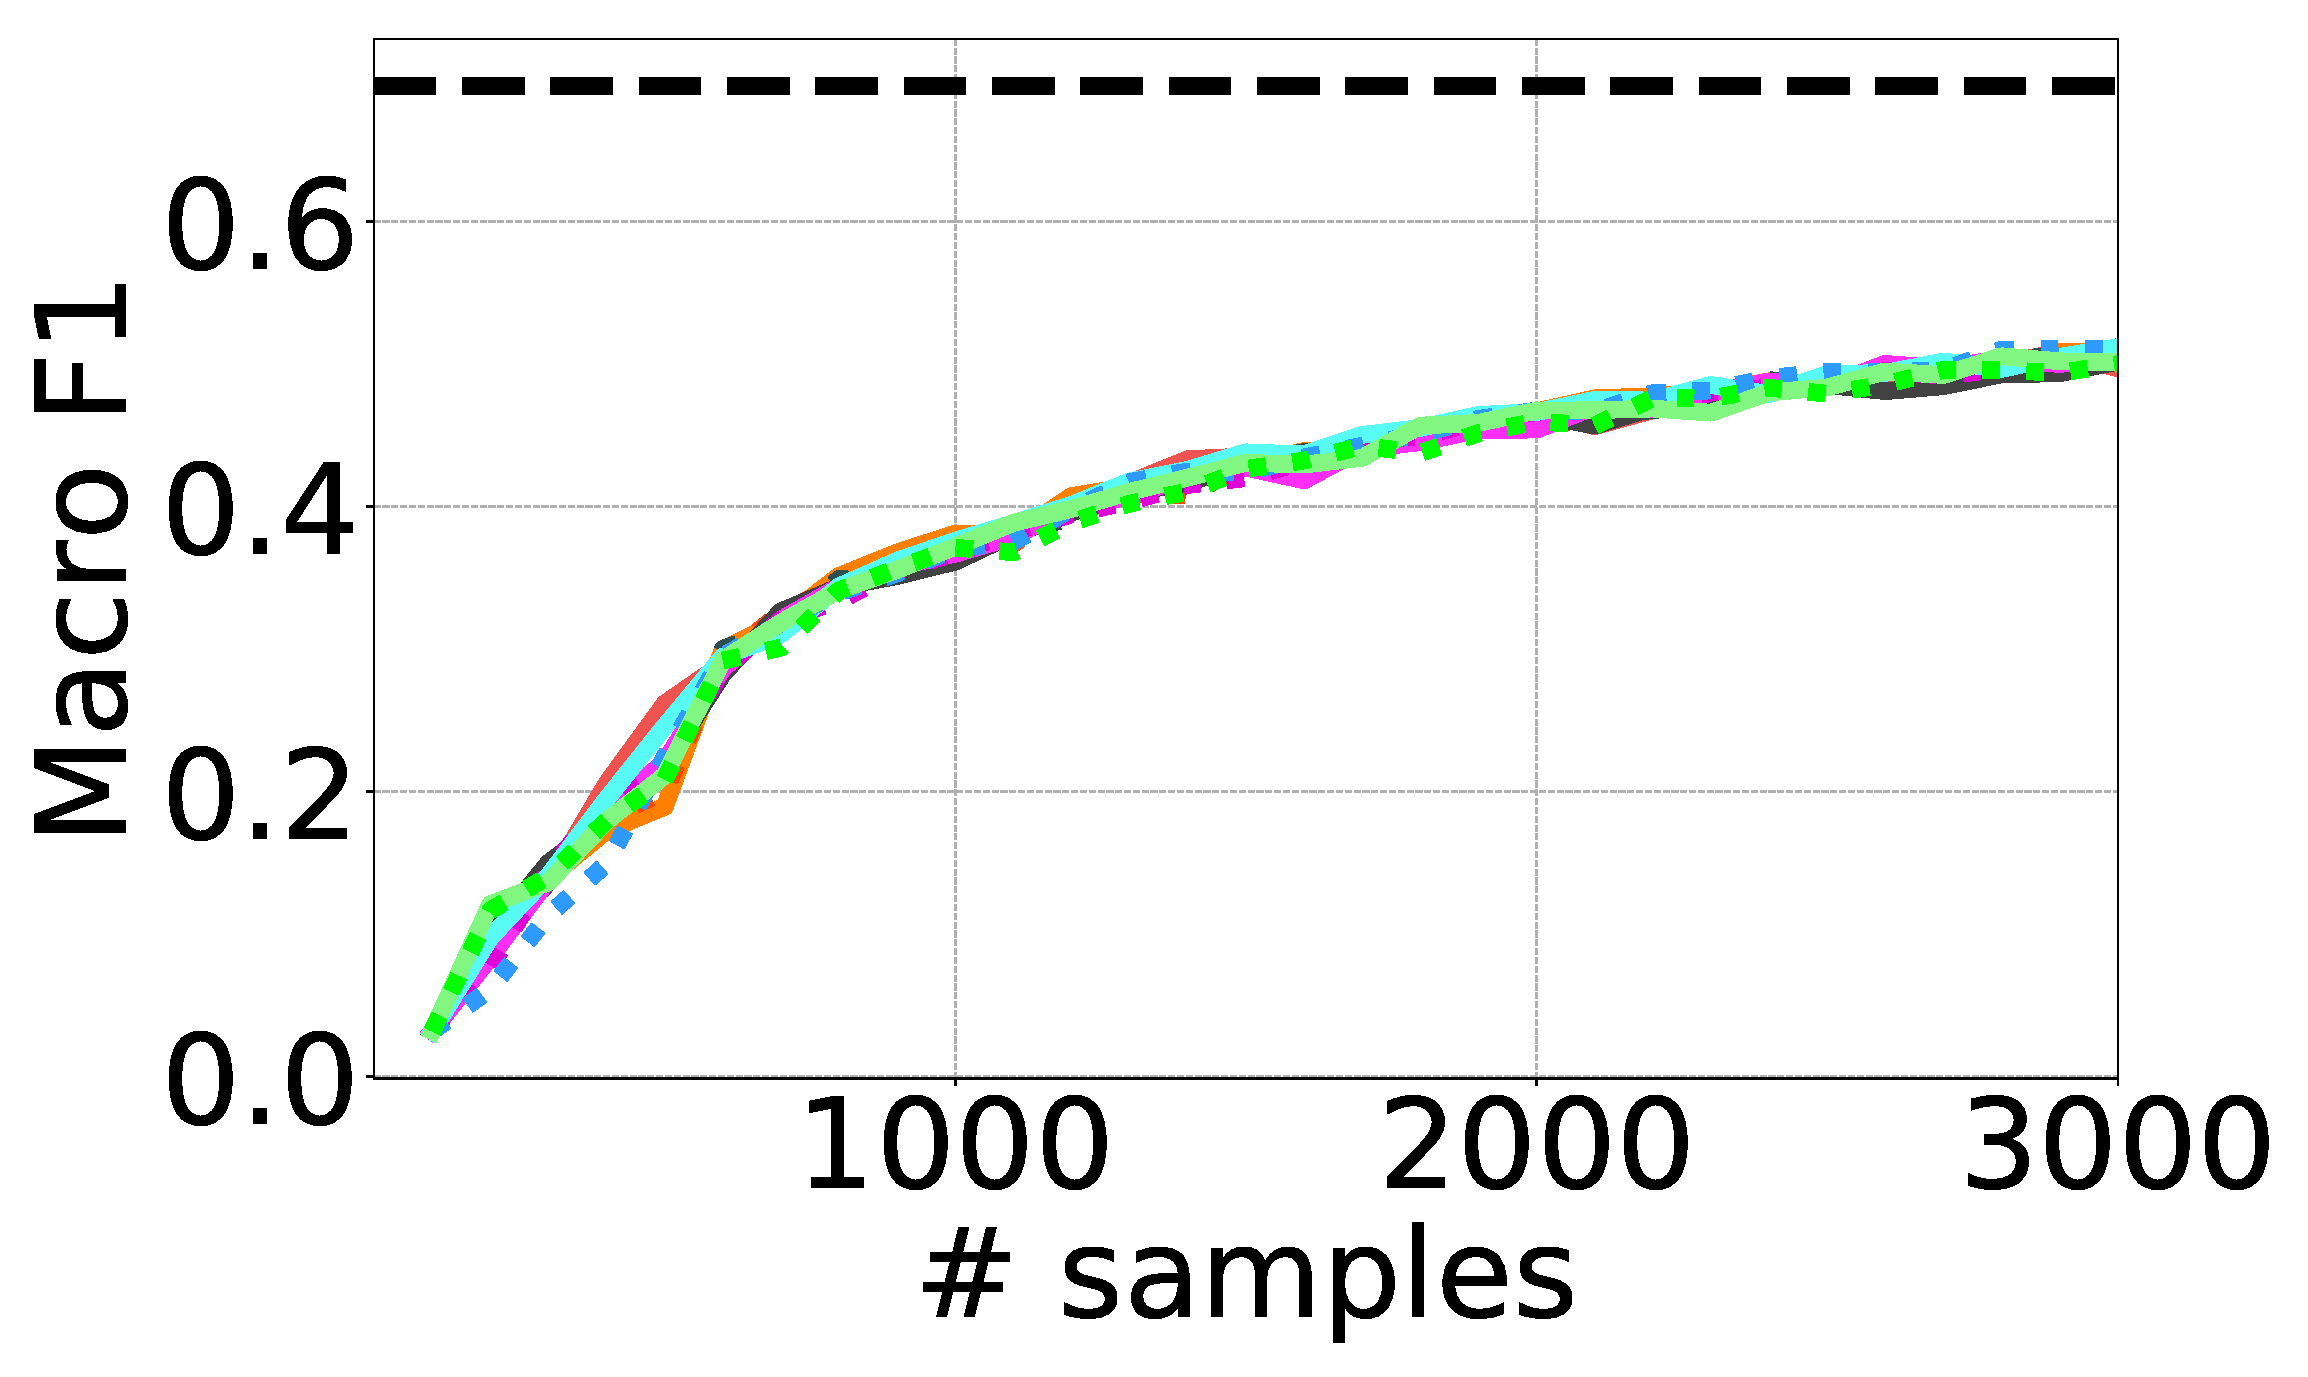
\includegraphics[width=0.23\textwidth]{res/cnn_pytorch_tnews_tokenized_acc_all.eps}} % \newline
		\subfloat[GCS]{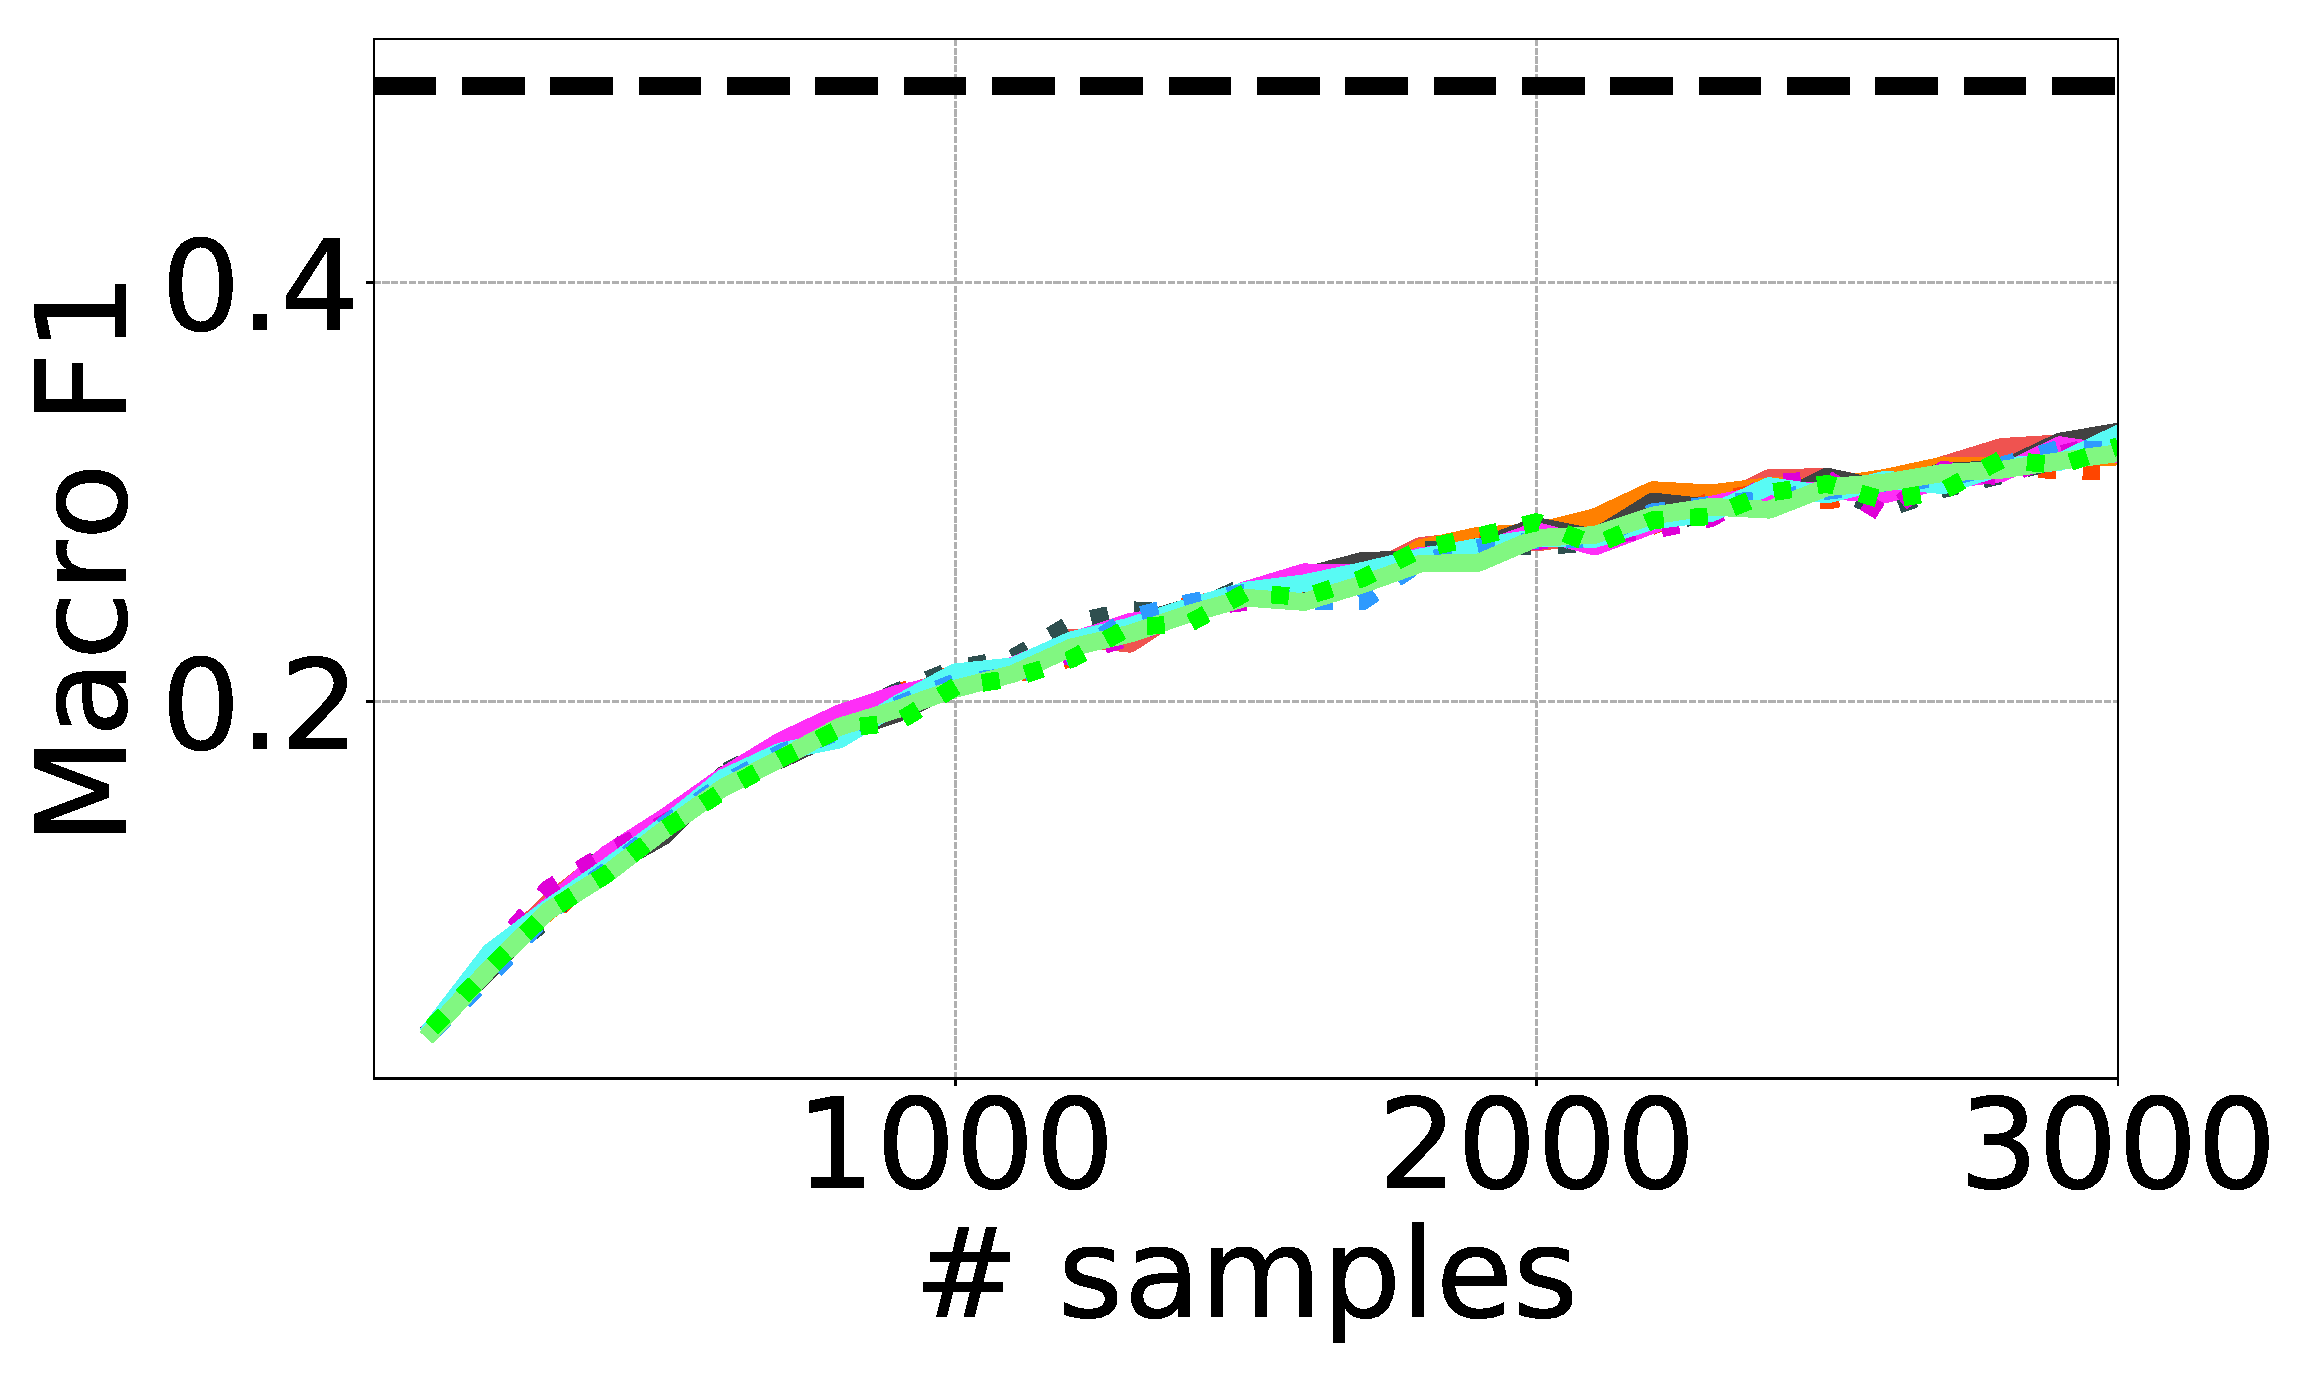
\includegraphics[width=0.23\textwidth]{res/cnn_pytorch_yanjing_tokenized_acc_all.eps}}
		\subfloat[Book]{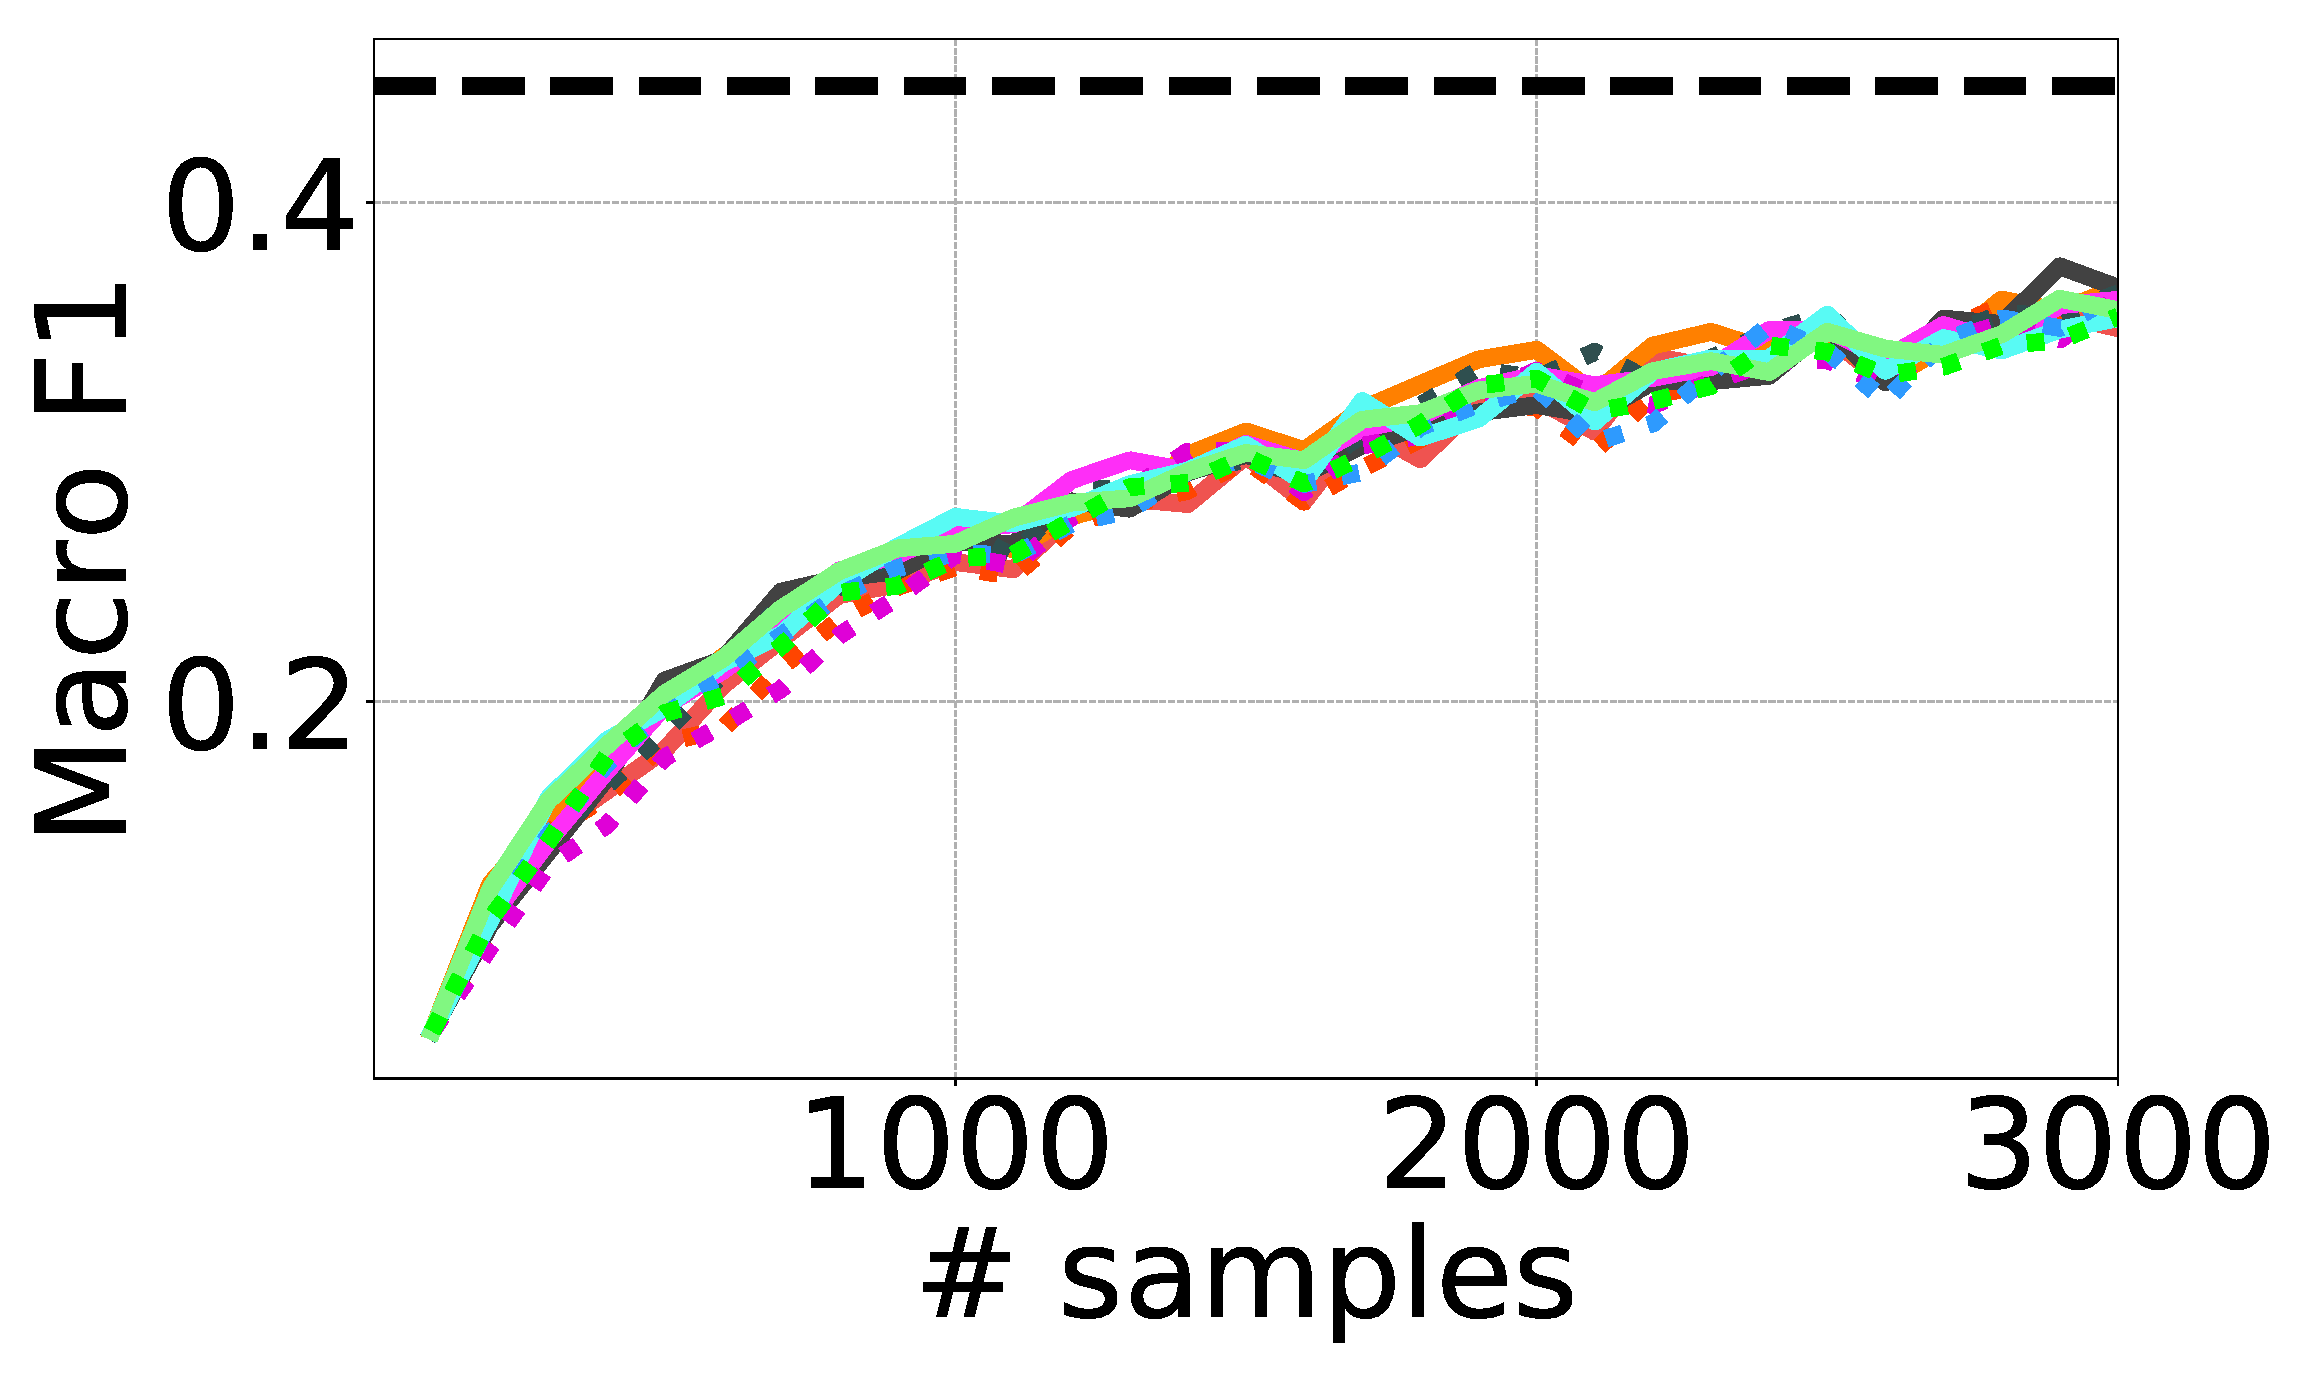
\includegraphics[width=0.23\textwidth]{res/cnn_pytorch_book_tokenized_acc_all.eps}}
	\end{center}
	\caption{Macro F1 curve of AL approaches on 8 datasets using CNN.}
	\label{fig:acc_all_cnn}
\end{figure*}


\subsubsection{Which classifier to choose?}
In order to determine which classifier is better to use with AL, we conduct same experiments on four popular classifiers. \Cref{fig:acc_all,fig:acc_all_bert,fig:acc_all_lstm,fig:acc_all_cnn} show AUC* of different strategies on fastText, CNN, LSTM as well as pretrained BERT. As depicted in the figures, 
the AUC* curves of CNN and LSTM are tightly entangled and 
sampling strategies show little advantage over the baseline random sampling, 
while fastText and BERT do show the difference. To quantify the margin gap 
of sampling strategies and random sampling in different classifiers, 
we calculate the ratio of best method to the random sampling on 
different classifiers in \tabref{table:ratioOfClassifiers}.

Similar to our observation from Figure 3-6, \tabref{table:ratioOfClassifiers} 
shows better classifiers are fastText and BERT. Although BRET also 
performs well for AL, the time cost to train the model is substantially
larger, compared with fastText. \tabref{table:trainingtime} shows that 
the average training time of BERT is 10 times longer than fastText. 
Therefore, we conclude that fastText is the more suitable classifier to use 
for AL on text classification.

\begin{table}[th]
	\small
	\centering
	\begin{tabular}{ccccccccc}
		\toprule
		Classifer & RT & HP & Bio & SS & EM & TN & GCS & BK\\ \hline
		fastText & \textbf{2.60} & \textbf{1.06} & 1.00 & \textbf{1.08} & 1.01 & 1.01 & 1.17 & 1.20\\
		BERT & 2.00 & 1.00 & 1.00 & 1.03 & \textbf{1.17} & \textbf{1.03} & \textbf{1.40} & \textbf{1.97}\\ 
		LSTM & 1.06 & 1.02 & \textbf{1.01} & 1.00 & 1.03 & 1.01 & 1.03 & 1.00\\
		CNN & 1.03 & 1.00 & \textbf{1.01} & 1.00 & 1.01 & 1.00 & 1.00 & 1.03\\		
		\bottomrule              
	\end{tabular}
\caption{AUC* ratio of best strategies to random sampling on datasets on four classifiers.}
\label{table:ratioOfClassifiers}
\end{table}
\begin{table}[th]
	\small
	\centering
	\begin{tabular}{ccccc}
% 		\toprule
% 		Classifer & AVG & Min & Max\\ \hline
% 		fastText & 20.7 & 12.2 & 29.3\\
% 		BERT & 204.0 & 200.6 & 214.2\\
% 		LSTM & 2.8 & 1.9 & 3.8\\
% 		CNN & 42.8 & 40.8 & 45.7\\ 
% 		\bottomrule  
		\toprule
		Time & fastText & BERT & LSTM & CNN\\ \hline
		AVG & 20.7 & 204.0 & 2.8 & 42.8  \\
		Min & 12.2 & 200.6 & 1.9 & 40.8\\
		Max & 29.3  & 214.2 & 3.8  & 45.7\\
		\bottomrule  
	\end{tabular}
	\caption{Training time on 3000 samples of four classifiers. \emph{AVG, Min, Max} is the average/minimum/maximum training time over 8 datasets. The values are in \emph{seconds}.}
	\label{table:trainingtime}
\end{table}

\begin{table}[!th]
	\small
	\centering
	\begin{tabular}{ccccccccc}
		\toprule
		\# of Classes  & RT & HP & Bio & SS & EM & TN & GCS & BK \\ \hline
		2  & 1.05  & 1.00 & \textbf{1.01} & 1.01 & 1.00 & 1.02  & 1.03 & 1.02\\
		5   & 1.07 & 1.00 & \textbf{1.01} & 1.04 & 1.03 & \textbf{1.03} & 1.03 & 1.06\\
		10 & 1.05 & 1.02 & \textbf{1.01} & - & \textbf{1.07} & \textbf{1.03}  & 1.05  &  1.01\\
		original  & \textbf{2.60} & \textbf{1.06} & 1.00 & \textbf{1.08} & 1.01 & 1.01  & \textbf{1.17}  & \textbf{1.20}\\ 
		\bottomrule              
	\end{tabular}
\caption{AUC* ratio of best strategies to random sampling on datasets on fastText with class number of 2,5,10 and all.}
\label{table:ratioOfDataset}
\end{table}



\subsubsection{Many-class or few-class?}
To illustrate the effect of the number of classes on AL performance, 
we conduct another experiment. We calculate the ratio of best strategy to 
the random sampling to show the effectiveness of active learning. 
We record the AUC* ratio of the original dataset as well as the subsets 
of the datasets with being only 2, 5 and 10 classes. This can be done by
filtering the dataset leaving only those data points with the top 2, 5 and 10 
class labels. 
%If in most cases, the original dataset has a great margin over subset dataset, 
%we can conclude the number of classes does an affect on active learning. 
%The more distinct class labels, the better the AL performance.
As \tabref{table:ratioOfDataset} shows, in almost all cases, 
the ratio increases with the number of classes, indicating that AL does work 
for many-class task, the more distinct class labels the better.

\subsubsection{Does the best sampling strategy exist?}
We would certainly hope to find an active learning strategy 
that outshines the rest on all datasets on all classifiers. 
Unfortunately, our experiments show otherwise: there is no clear winner 
for the datasets we evaluated. 

Even if we analyze the results on a single classifier, 
the best strategy varies. For example, according to the AUC* on 
fastText in \tabref{table:auc_ft}, we can't find a method which outperforms 
other on all datasets.  However, if we only compare a strategy with
or without the frequency tuning, conclusion can be made. We calculate the average AUC* of each strategy and also sort the AUC* on each dataset in 
descending order and calculate the MRR of 
each sampling strategies.
\begin{equation}
    AVG(method) = \frac{1}{|Q|}\sum_{i=1}^{|Q|}AUC*_i^{method},
\end{equation}
\begin{equation}
    MRR(method) = \frac{1}{|Q|}\sum_{i=1}^{|Q|}\frac{1}{rank_i^{method}},
\end{equation}
where in our experiment, $Q$ denotes the number of datasets we want to compare, $rank_i^{method}$ means the AUC* ranking of $method$ on dataset $i$. ${AUC^*}^{method}_{i}$ is the AUC* of $method$ on $dataset_i$.
The larger the MRR and the AVG, the better the performance. In \tabref{table:auc_ft}, 
except for least confidence sampling, all other strategies show improvement
with the class frequency tuning on both AVG and MRR.
Also, K-center greedy with frequency works the best with fastText.

\begin{table*}[th]
	\centering
	\small
	\begin{tabular}{ccccccccc|cc}
		\toprule
Method & Reuters & HuffPost & Biomedical & SearchSnippets & Emoji & TNEWS & GCS & Book & AVG & MRR\\ \hline
Random Sampling & 365.96 & 553.08 & 1601.06 & 2397.09 & 355.35 & 1673.69 & 892.04 & 965.12 & 1100.42 & 1.82\\ \hline
Least Confidence & \textbf{1003.46} & 510.76 & 1448.65 & \textbf{2577.79} & 321.99 & 1597.56 & 900.37 & 1116.35 & 1184.62 & 2.71\\
LC with Freq & 947.62 & 511.51 & 1457.55 & 2560.64 & 320.41 & 1701.79 & 945.64 & 1077.4 & \underline{1190.32} & 1.22\\ \hline
K-center Greedy & 761.08 & 525.58 & 1428.09 & 2542.13 & \textbf{357.15} & 1555.7 & 901.12 & 1004.73 & 1134.45 & 1.86\\
KG with Freq & 777.75 & \textbf{563.45} & \textbf{1607.86} & 2537.36 & 347.68 & \textbf{1725.67} & 1033.42 & 1132.34 & \underline{1215.69} & \textbf{\underline{4.01}}\\ \hline        
Uncertainty Sampling & 957.36 & 505.95 & 1466.59 & 2569.79 & 315.03 & 1694.25 & 980.86 & 1096.8 & 1198.33 & 1.77\\
US with Freq & 950.81 & 545.73 & 1570.32 & 2517.53 & 346.17 & 1717.1 & 1063.07 & \textbf{1161.62} & \textbf{\underline{1234.04}} & \underline{2.88}\\ \hline
Weighted Uncertainty & 844.36 & 537.29 & 1489.05 & 2518.29 & 309.94 & 1672.12 & 1045.88 & 1135.19 & 1194.01 & 1.31\\
WU with Freq & 927.6 & 553.26 & 1547.8 & 2511.87 & 339.43 & 1685.87 & 1078.72 & 1150.2 & \underline{1224.34} & \underline{2.29}\\ \hline
Radius Uncertainty & 936.43 & 523.49 & 1524.43 & 2568.68 & 321.09 & 1702.76 & 1009.78 & 1090.55 & 1209.65 & 1.48\\
RU with Freq & 953.28 & 523.47 & 1562.1 & 2516.44 & 331.15 & 1725.12 & \textbf{1080.33} & 1147.4 & \underline{1229.91} & \underline{2.82}\\ \hline
	\end{tabular}
\caption{AUC* of sampling strategies on seven datasets running from 100 to 3000 with batch size 100 using fastText. For AVG and MRR, 
the strategies that benefit from frequency tuning are underlined.}
\label{table:auc_ft}
\end{table*}


\subsubsection{Which AL strategy for which dataset?}
Since the performance of sampling strategies vary on different datasets, it is natural for us to aim to figure out which characteristics of datasets will affect the results. We mainly try to find out the correlation between performance of sampling strategies and characteristics of datasets like average text length of samples, size of datasets and class distribution.

We calculate the standard deviation of the sizes of all labels to describe the class distribution of different datasets. Average text length and dataset size are shown in \tabref{table:statsOfDataset}.  We calculate the Spearman's rank correlation using the AUC* of sampling strategies and the characteristics of eight datasets. For example, the formula to calculate the relation between random sampling and average text length of datasets is shown as follows,
\begin{equation}
    \rho = 1 - \frac{6\sum_i(avg\_len_i - {AUC^*}^{Random}_{i})}{n(n^2 - 1)},
\end{equation}
where $i$ denotes for one of the 8 datasets and $n$ equals to the total number of datasets, 
and in our case is 8. ${AUC^*}^{Random}_{i}$ is the AUC* of random sampling on $dataset_i$.

As \tabref{table:correkationOfDataset} shows, size of dataset and class distribution have weak correlation with the AL performance since the absolute value of Spearman's correlations are less than 0.39, while average text length of samples have moderate correlation to AL performance (less than 0.6). All these features don't have strong correlation to the performance. Thus in practice, given a dataset, we can't pre-determine a theoretically suitable sampling strategy without 
running some tests.

\begin{table*}[th]
	\small
	\centering
	\begin{tabular}{cccccccccccc}
		\toprule
		 &  R & LC & LC with Freq & KG & KG with Freq & US & US with Freq & WU & WU with Freq & RU & RU with Freq\\\hline
		Avg Tokens/sample & 0.38 & 0.38 & 0.38 & \textbf{0.42} & \textbf{0.42} & 0.38 & 0.38 & 0.31 & 0.38 & 0.38 & 0.38 \\
		\#Samples & -0.24 & \textbf{-0.33} & \textbf{-0.33} & -0.24 & -0.24 & -0.24 & -0.24 & -0.21 & -0.24 &-0.24 & -0.24\\
		Distribution & -0.24 & \textbf{-0.29} &\textbf{ -0.29} & -0.24 & -0.24 & -0.24 & -0.24 & -0.21 & -0.24 & -0.24& -0.24 \\ 
		\bottomrule              
	\end{tabular}
\caption{Spearman's correlation between average tokens per sample, number of samples and normal distribution of classes on eight datasets with AUC* of 11 sampling strategies.}
\label{table:correkationOfDataset}
\end{table*}

%\begin{figure}[th]
%	\centering
%	\includegraphics[scale=0.3]{figs/all_radiusfreq.pdf}
%	\caption{Training using Random Uncertainty with Freq}
%	\label{fig:all_radiusfreq}
%\end{figure}
% \begin{table}[th]
% 	\scriptsize
% 	\centering
% 	\begin{tabular}{ccc}
% 		\toprule
% 		Dataset & \% of All Training Samples & Required Samples \\ \hline
% 		Reuters & 82.08   &  6,200 \\
% 		SQD     & 28.44   &  9,100 \\
% 		TNEWS   & 20.57    &  55,100 \\
% 		GCS     & 68.09   &  35,100 \\
% 		Biomedical & 43.13 & 6,900\\
% 		StackOverflow & 3.44 &550 \\
% 		SearchSnippets & 24.31 & 2,400 \\
% 		\bottomrule
% 	\end{tabular}
% 	\caption{\% samples and \# samples required to reach 95\% of the best accuracy (using fastText)}
% 	\label{table:all_radiusfreq}
% \end{table}


% \begin{table*}[th]
% 	\centering
% 	\scriptsize
% 	\begin{tabular}{ccccccccc}
% 		\toprule
% 		Method & Reuters & HuffPost & Biomedical & SearchSnippets & Emoji & TNEWS & GCS & Book\\ \hline
% 		Random Sampling & 735.48 & \textbf{631.47} & 1645.23 & 2635.49 & 311.04 & 2165.06 & 722.41 & 607.93\\ \hline
% 		Least Confidence & 1457.27 & 413.61 & 1646.54 & 2701.42 & 319.47 & 2209.68 & \textbf{1011.2} & \textbf{1196.92}\\
% 		LC with Freq & 1236.85 & 389.19 & 1622.93 & 2642.65 & 330.05 & 2186.32 & 862.58 & 882.74\\
% 		LC with Sqrtfreq & 1380.05 & 393.7 & 1608.29 & 2671.16 & 318.57 & 2197.42 & 940.76 & 1006.02\\ \hline
% 		K-center Greedy & 1071.54 & 367.29 & 1498.01 & 2699.18 & 283.0 & 2180.65 & 706.6 & 917.25\\
% 		KG with Freq & 1313.01 & 396.13 & 1549.57 & \textbf{2708.4} & 357.83 & 2203.54 & 851.51 & 1021.27\\
% 		KG with Sqrtfreq & 1234.28 & 412.43 & 1591.73 & 2697.86 & \textbf{371.16} & 2188.17 & 830.44 & 992.39\\ \hline
% 		Uncertainty Sampling & 1473.7 & 439.76 & 1618.5 & 2705.07 & 334.16 & 2209.74 & 995.06 & 1175.11\\
% 		US with Freq & 1429.87 & 415.87 & 1642.42 & 2699.62 & 350.13 & 2197.19 & 855.54 & 1038.68\\
% 		US with Sqrtfreq & 1468.11 & 401.2 & \textbf{1654.19} & 2693.02 & 357.98 & 2199.49 & 899.07 & 1082.11\\ \hline
% 		Weighted Uncertainty & 1373.0 & 376.95 & 1563.85 & 2688.95 & 365.16 & 2195.93 & 793.33 & 998.61\\
% 		WU with Freq & 1413.31 & 357.99 & 1620.71 & 2691.48 & 362.79 & 2181.9 & 762.84 & 975.13\\
% 		WU with Sqrtfreq & 1403.26 & 366.0 & 1626.65 & 2693.51 & 370.73 & 2179.43 & 786.64 & 976.79\\ \hline
% 		Radius Uncertainty & \textbf{1488.56} & 438.08 & 1603.47 & 2696.04 & 341.99 & \textbf{2213.75} & 987.74 & 1193.83\\
% 		RU with Freq & 1450.33 & 408.85 & 1623.07 & 2693.76 & 350.15 & 2198.52 & 922.56 & 1038.41\\
% 		RU with Sqrtfreq & 1447.41 & 396.9 & 1640.04 & 2703.63 & 367.38 & 2200.49 & 869.24 & 1106.71\\ \hline
% 	\end{tabular}
% \caption{AUC* of sampling strategies on seven datasets up to 3000 samples using BERT (need update HuffPost)}
% \label{table:auc_bert}
% \end{table*}

% \begin{table*}[th]
% 	\centering
% 	\scriptsize
% 	\begin{tabular}{ccccccccc}
% 		\toprule
% 		Method & Reuters & HuffPost & Biomedical & SearchSnippets & Emoji & TNEWS & GCS & Book\\ \hline
% 		Random Sampling & 1171.85 & 356.05 & 1678.61 & 2574.88 & 325.49 & 1134.52 & 682.51 & 796.48\\ \hline
% 		Least Confidence & 1135.6 & 374.37 & 1680.56 & 2567.71 & 329.54 & 1129.27 & 678.87 & 823.07\\
% 		LC with Freq & 1131.98 & 348.28 & 1678.93 & 2565.62 & 320.68 & 1110.4 & 682.37 & 806.92\\
% 		LC with Sqrtfreq & \textbf{1191.21} & 353.76 & 1680.81 & \textbf{2583.16} & 327.63 & 1128.68 & 687.8 & 787.63\\ \hline
% 		K-center Greedy & 1152.38 & 370.74 & 1675.29 & 2576.36 & 323.76 & 1118.54 & 677.7 & 808.12\\
% 		KG with Freq & 1145.88 & 366.11 & 1682.51 & 2575.76 & 322.12 & 1131.99 & \textbf{692.8} & \textbf{839.18}\\
% 		KG with Sqrtfreq & 1171.33 & 366.21 & 1677.66 & 2573.71 & 322.21 & 1124.21 & 677.2 & 806.95\\ \hline
% 		Uncertainty Sampling & 1138.71 & 362.75 & 1674.35 & 2581.85 & 316.69 & 1120.9 & 679.54 & 817.39\\
% 		US with Freq & 1154.66 & 357.9 & 1682.91 & 2569.95 & 329.54 & 1116.91 & 672.61 & 801.9\\
% 		US with Sqrtfreq & 1140.45 & 364.12 & 1680.8 & 2574.77 & 325.26 & \textbf{1141.35} & 691.65 & 821.05\\ \hline
% 		Weighted Uncertainty & 1178.2 & \textbf{376.45} & \textbf{1696.91} & 2575.85 & 329.27 & 1138.16 & 676.96 & 812.7\\
% 		WU with Freq & 1105.28 & 360.02 & 1685.69 & 2577.46 & 323.38 & 1124.96 & 678.15 & 805.31\\
% 		WU with Sqrtfreq & 1143.39 & 366.89 & 1671.53 & 2572.86 & 316.65 & 1121.13 & 680.5 & 798.16\\ \hline
% 		Radius Uncertainty & 1137.96 & 361.3 & 1675.82 & 2572.12 & \textbf{334.4} & 1137.94 & 683.7 & 805.41\\
% 		RU with Freq & 1162.03 & 362.68 & 1666.85 & 2579.86 & 330.85 & 1126.01 & 682.56 & 810.49\\
% 		RU with Sqrtfreq & 1103.03 & 355.3 & 1681.99 & 2572.51 & 321.07 & 1110.42 & 675.38 & 814.03\\ \hline
% 	\end{tabular}
% \caption{AUC* of sampling strategies on seven datasets up to 3000 samples using CNN}
% \label{table:auc_cnn}
% \end{table*}


% \begin{table*}[th]
% 	\centering
% 	\scriptsize
% 	\begin{tabular}{ccccccccc}
% 		\toprule
% 		Method & Reuters & HuffPost & Biomedical & SearchSnippets & Emoji & TNEWS & GCS & Book\\ \hline
% 		Random Sampling & 967.97 & 384.44 & 1621.04 & \textbf{2556.06} & 317.09 & 1068.78 & 647.57 & 752.89\\ \hline
% 		Least Confidence & 1004.14 & 372.5 & 1618.59 & 2547.06 & 313.9 & 1075.34 & 657.38 & 719.13\\
% 		LC with Freq & 1039.73 & 373.99 & 1631.81 & 2548.83 & 307.91 & 1075.89 & 638.37 & 707.19\\
% 		LC with Sqrtfreq & 983.85 & 371.24 & 1622.49 & 2553.09 & 310.79 & 1078.52 & 647.46 & 751.82\\ \hline
% 		K-center Greedy & 991.42 & 377.23 & 1614.37 & 2544.96 & 302.66 & 1067.47 & \textbf{667.1} & 740.22\\
% 		KG with Freq & 964.34 & 377.54 & 1618.1 & 2551.58 & 322.58 & 1073.61 & 634.71 & 734.0\\
% 		KG with Sqrtfreq & 1021.28 & \textbf{389.99} & 1611.84 & 2549.26 & 314.6 & 1062.41 & 656.75 & 746.59\\ \hline
% 		Uncertainty Sampling & 946.19 & 376.03 & 1637.26 & 2539.56 & \textbf{325.55} & 1074.99 & 650.14 & 753.85\\
% 		US with Freq & 996.26 & 381.41 & 1619.85 & 2546.41 & 311.84 & 1078.46 & 645.45 & 747.56\\
% 		US with Sqrtfreq & 1009.67 & 383.92 & 1617.3 & 2539.38 & 308.68 & 1079.33 & 650.56 & 723.11\\ \hline
% 		Weighted Uncertainty & 972.58 & 382.46 & 1631.22 & 2551.66 & 313.79 & 1078.31 & 654.93 & 748.21\\
% 		WU with Freq & 1028.6 & 381.2 & \textbf{1642.74} & 2543.95 & 322.9 & 1075.1 & 657.96 & 723.93\\
% 		WU with Sqrtfreq & 966.16 & 379.39 & 1624.52 & 2547.77 & 316.39 & 1082.51 & 658.42 & 722.91\\ \hline
% 		Radius Uncertainty & \textbf{1052.84} & 384.97 & 1629.98 & 2548.66 & 309.41 & 1069.68 & 665.18 & \textbf{754.01}\\
% 		RU with Freq & 982.6 & 386.33 & 1624.4 & 2548.12 & 309.75 & 1063.08 & 637.45 & 744.45\\
% 		RU with Sqrtfreq & 945.36 & 380.38 & 1609.52 & 2550.56 & 312.38 & \textbf{1093.31} & 651.87 & 752.36\\
% 		\hline
% 	\end{tabular}
% \caption{AUC* of sampling strategies on seven datasets running from 100 to 3000 with batch size 100 using LSTM}
% \label{table:auc_lstm}
% \end{table*}

% \begin{table}[th]
% 	\centering
% 	\scriptsize
% 	\begin{tabular}{ccccc}
% 		\toprule
% 		Method & BERT & fastText & CNN & LSTM \\  \hline
% 		Random Sampling       & 1.72 & 1.24 & 1.26 & 2.2\\ \hline
% 		Least Confidence      & \textbf{3.91} & \textbf{2.55} & 1.87 & 0.95\\
% 		LC with Freq          & 0.73 & 1.02 & 0.68 & 1.39\\
% 		LC with Sqrtfreq      & 0.91 & 0.88 & 2.94 & 1.42\\ \hline
% 		K-center Greedy       & 0.63 & 1.51 & 1.15 & 1.59\\
% 		KG with Freq          & 1.85 & 2.36 & 2.97 & 1.07\\
% 		KG with Sqrtfreq      & 1.64 & 2.38 & 1.02 & 2.0\\ \hline
% 		Weighted Uncertainty  & 2.86 & 1.2 & 1.3 & 2.41\\
% 		WU with Freq          & 1.2 & 1.4 & 1.12 & 0.99\\
% 		WU with Sqrtfreq      & 2.32 & 2.03 & 2.46 & 1.13\\ \hline
% 		Uncertainty Sampling  & 0.84 & 1.77 & \textbf{3.6} & 1.44\\
% 		US with Freq          & 0.87 & 2.08 & 1.29 & 2.47\\
% 		US with Sqrtfreq      & 1.18 & 1.16 & 0.87 & 1.55\\ \hline
% 		Radius Uncertainty    & 3.39 & 1.33 & 2.02 & \textbf{3.32}\\
% 		RU with Freq          & 1.21 & 1.85 & 1.67 & 1.18\\
% 		RU with Sqrtfreq      & 1.79 & 2.28 & 0.83 & 1.92\\
% 		\hline
% 	\end{tabular}
% 	\caption{MRR score of sampling strategies on seven datasets using different classifiers.}
% 	\label{table:mrr}
% \end{table}



% Since frequency adjustment is specially designed for many-class scenarios, 
% we only compare the MRR scores on the original datasets. 
% As \figref{fig:mrr} shows, all the orange and green bars are higher than the blue bars. 
% In other words, strategies have increased their score to some extent after applying frequency 
% adjustment regardless of the ending point.

% \begin{figure*}
% 	\centering
% 	%\subfloat[Complaint]{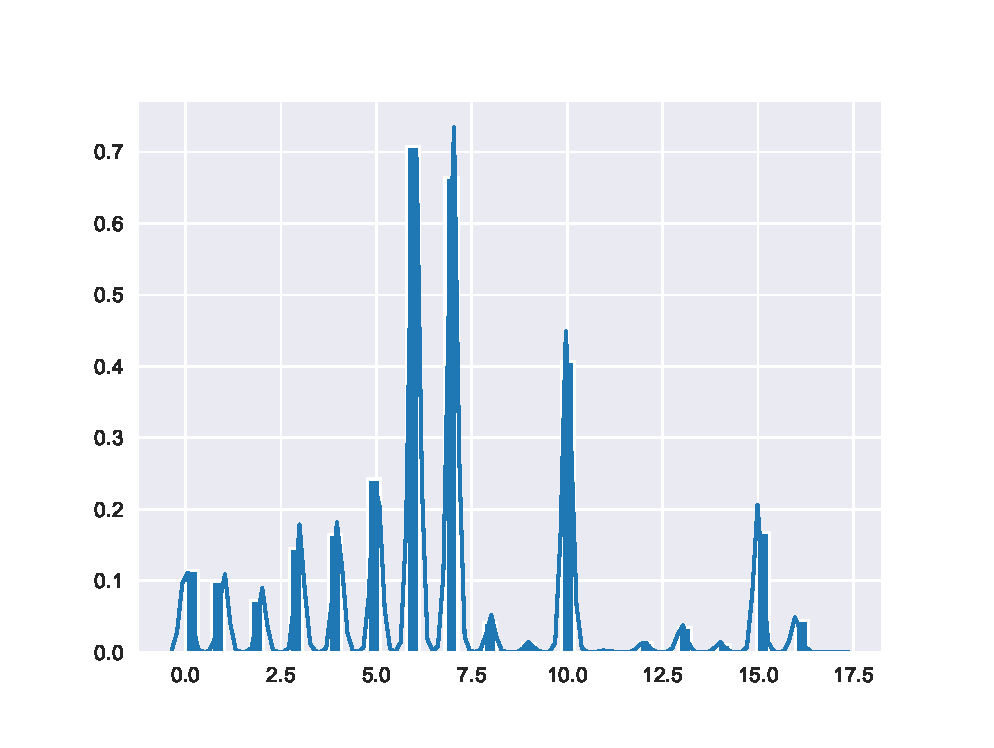
\includegraphics[width=0.2\textwidth]{figs/complaint.eps}}
% 	\subfloat[AL up to 1000 samples]{\includegraphics[width=0.3\textwidth]{figs/mrr_1000.pdf}}
% 	\subfloat[AL up to 2000 samples]{\includegraphics[width=0.3\textwidth]{figs/mrr_2000.pdf}}
% 	\subfloat[AL up to 3000 samples]{\includegraphics[width=0.3\textwidth]{figs/mrr_3000.pdf}}
% 	\caption{MRR scores before and after applying frequency adjustment on WU, US and RU. EP = 1000,2000,3000 denotes for AL up to 1000,2000,3000 respectively.} 
% 	\label{fig:mrr}
% \end{figure*}

% \begin{figure}[th]
% 	\centering
% 	\subfloat[][
% 	Drop of MRR score of tradition sampling strategies]{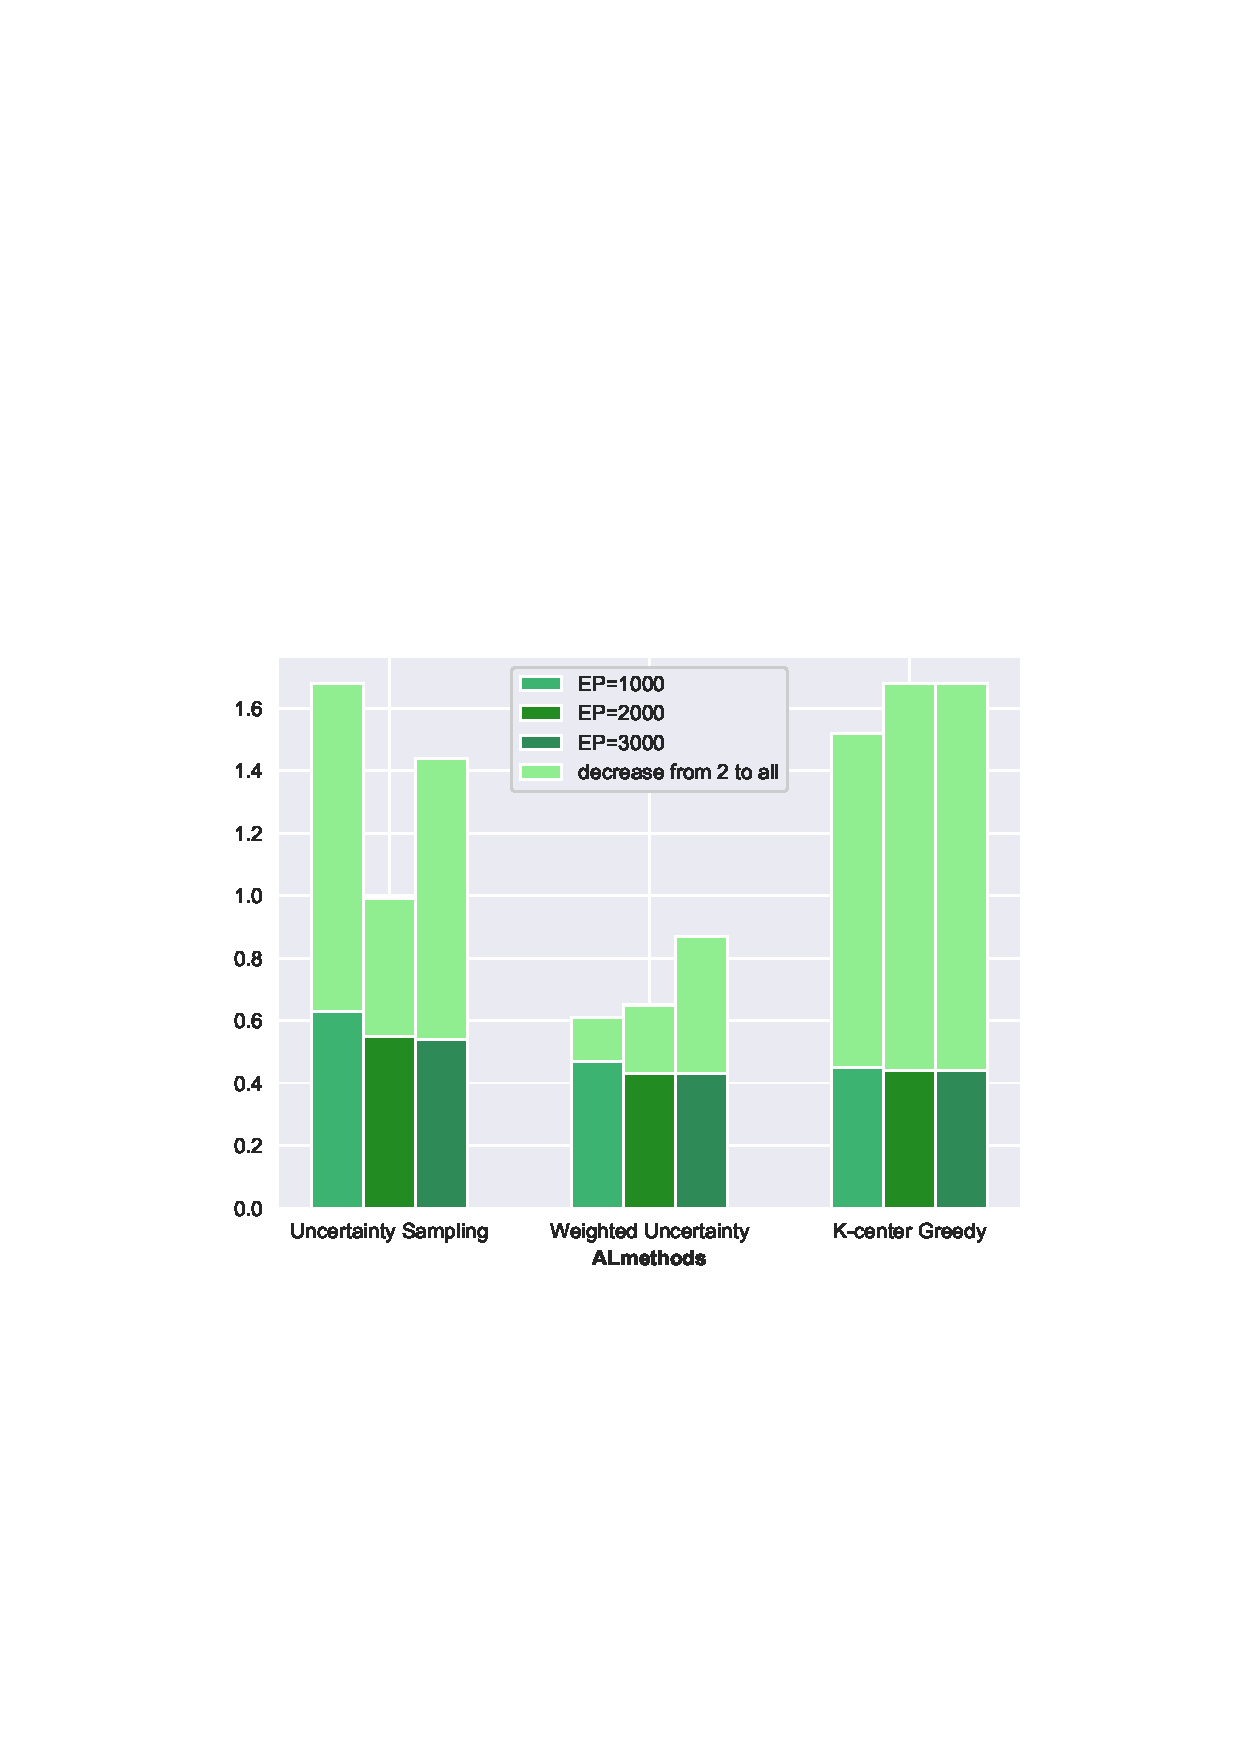
\includegraphics[width=0.25\textwidth]{figs/drop.pdf}}
% 	\subfloat[][ 
% 	Increase of MRR score of Radius-based strategies
% 	($\triangledown$ indicates decreasing)]{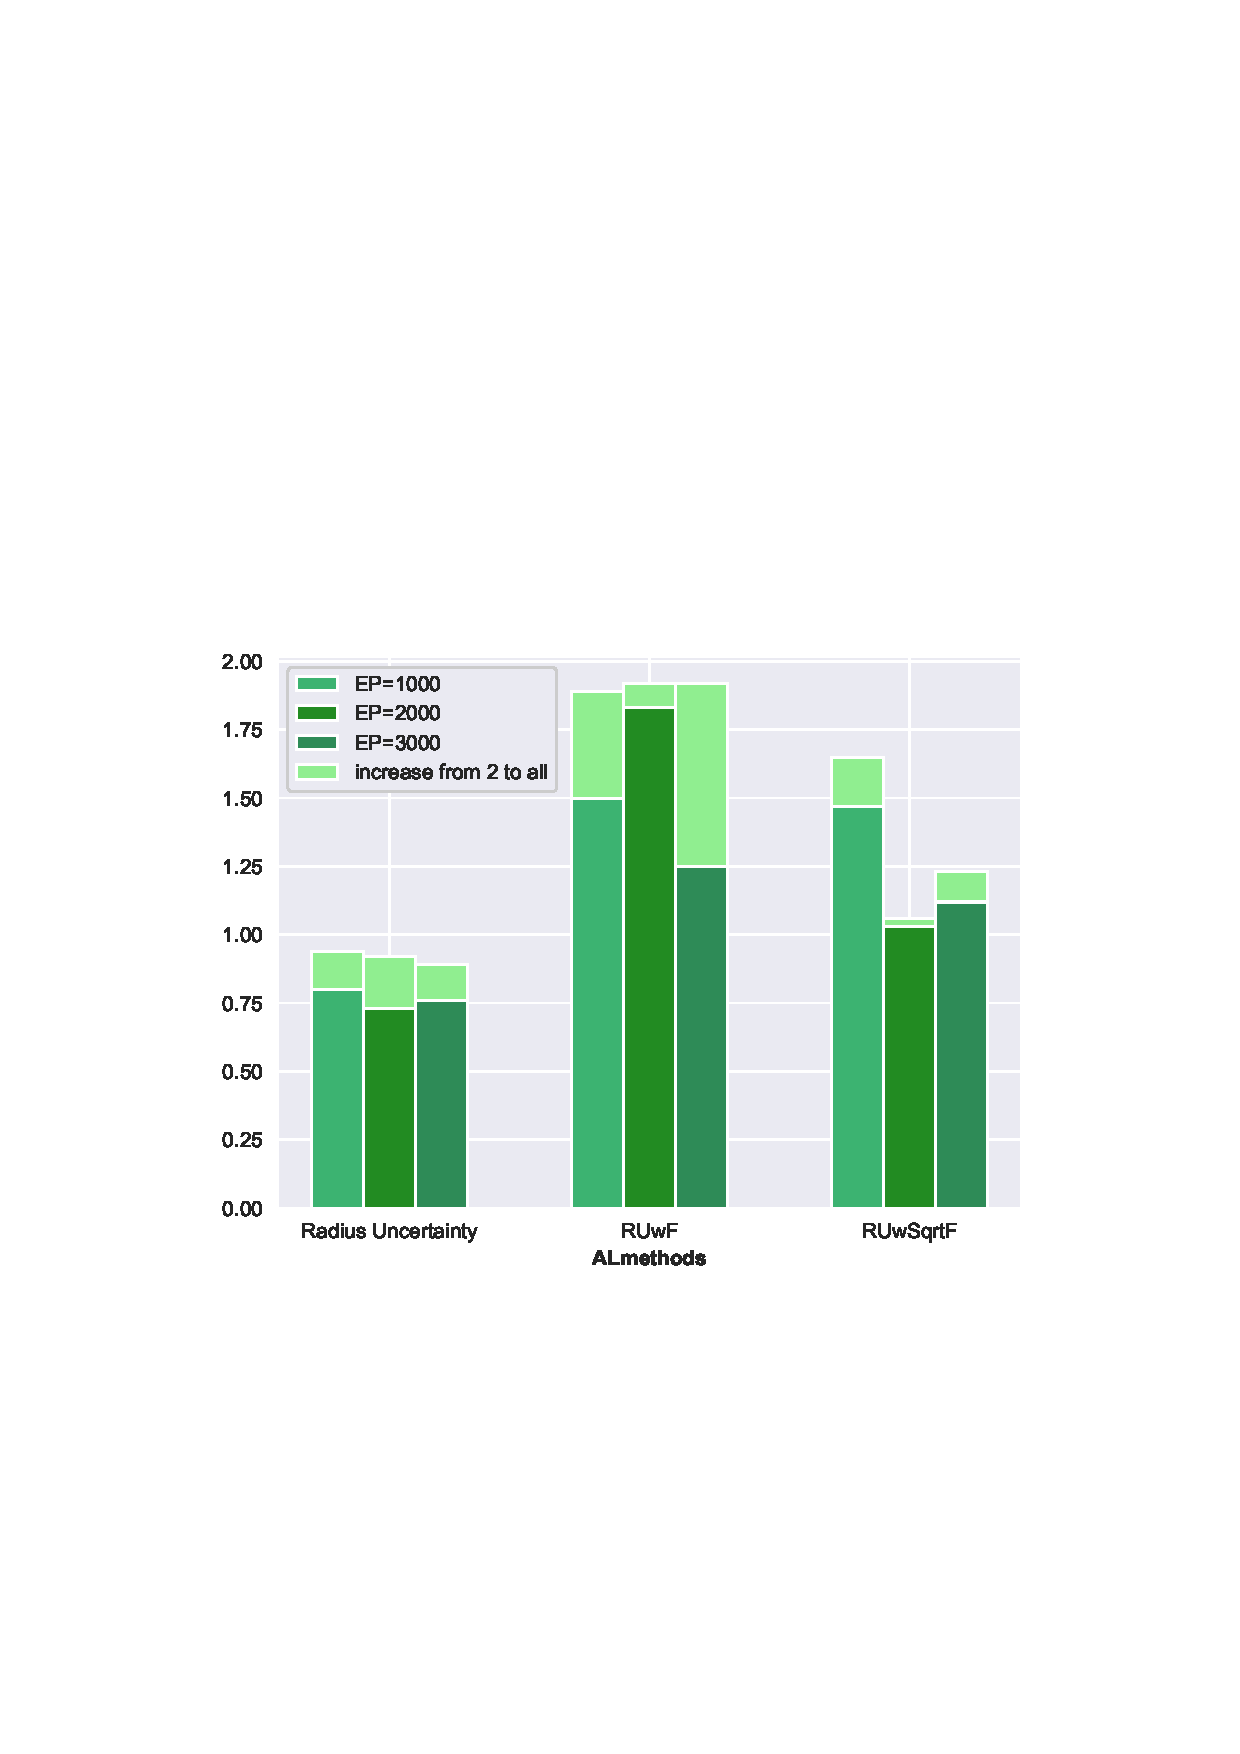
\includegraphics[width=0.25\textwidth]{figs/plus.pdf}}
% 	\caption{Difference in MRR scores between 2-class and all-class problems  (F is Freq and SqrtF is Sqrtfreq)}
% 	\label{fig:trend}
% \end{figure}

% \subsection{Effects of Frequency Adjustment}
% Figure ~\ref{fig:legend} shows the legend of all result figures. 
% Figure ~\ref{fig:complaint_exp1},~\ref{fig:reuters_exp1},~\ref{fig:so_exp1},~\ref{fig:tnews_exp1},~\ref{fig:yanjing_exp1} display Experiment (a) results and Figure ~\

% \begin{figure}[h]
% 	\centering
% 	\includegraphics[scale=0.5]{figs/legend.pdf}
% 	\caption{Legend of Result Figures. In following figures, 
% unless otherwise noted, \textit{x} denotes the size of training samples 
% and \textit{y} denotes macro-average F1 score of the classifier trained
% on the corresponding trainig sample.}
% 	\label{fig:legend}
% \end{figure}

% \begin{figure}[h]
% 	\includegraphics[scale=0.5]{figs/complaint_exp1.pdf}
% 	\caption{Exp (a) Result of Complaint. From left to right, from upper to lower is 2, 5, 10 and all classes.}
% 	\label{fig:complaint_exp1}
% \end{figure}

% \begin{figure}[h]
% 	\includegraphics[scale=0.5]{figs/reuters_exp1.pdf}
% 	\caption{Exp (a) Result of Reuters}
% 	\label{fig:reuters_exp1}
% \end{figure}

% \begin{figure}[h]
% 	\includegraphics[scale=0.5]{figs/so_exp1.pdf}
% 	\caption{Exp (a) Result of SO}
% 	\label{fig:so_exp1}
% \end{figure}

% \begin{figure}[h]
% 	\includegraphics[scale=0.5]{figs/tnews_exp1.pdf}
% 	\caption{Exp (a) Result of TNEWS}
% 	\label{fig:tnews_exp1}
% \end{figure}

% \begin{figure}[h]
% 	\includegraphics[scale=0.5]{figs/yanjing_exp1.pdf}
% 	\caption{Exp (a) Result of GCS}
% 	\label{fig:yanjing_exp1}
% \end{figure}


% \subsection{Radius vs. Other state-of-the-art strategies}
% \KZ{Here we show the results of applying freq to various
% base sampling strategies.}

% \begin{figure}[h]
% 	\includegraphics[scale=0.5]{figs/complaint_exp2.pdf}
% 	\caption{Exp (b) Result of Complaint}
% 	\label{fig:complaint_exp2}
% \end{figure}

% \begin{figure}[h]
% 	\includegraphics[scale=0.5]{figs/reuters_exp2.pdf}
% 	\caption{Exp (b) Result of Reuters}
% 	\label{fig:reuters_exp2}
% \end{figure}

% \begin{figure}[h]
% 	\includegraphics[scale=0.5]{figs/so_exp2.pdf}
% 	\caption{Exp (b) Result of SO}
% 	\label{fig:so_exp2}
% \end{figure}

% \begin{figure}[h]
% 	\includegraphics[scale=0.5]{figs/tnews_exp2.pdf}
% 	\caption{Exp (b) Result of TNEWS}
% 	\label{fig:tnews_exp2}
% \end{figure}

% \begin{figure}[h]
% 	\includegraphics[scale=0.5]{figs/yanjing_exp2.pdf}
% 	\caption{Exp (b) Result of GCS}
% 	\label{fig:yanjing_exp2}
% \end{figure}

% \begin{table}[]
% 	\begin{tabular}{cc|cc}
% 		\hline
% 		Method           & Score  & Method           & Score\\ \hline
% 		Random           & 2.40 & Density           & 2.73 \\
% 		Active           & 3.11 &  Density freq     & 4.12  \\
% 		Center           & 5.52 &  Density sqrtfreq & 3.43  \\
% 		Entropy          & 6.89 &  Radius           & 5.57  \\
% 		Entropy freq     & 7.83 &  Radius freq      & 6.83  \\
% 		Entropy sqrtfreq & 6.21 &  Radius sqrtfreq  & 7.44  \\ \hline
% 	\end{tabular}
% \caption{Score of strategies summed over datasets and number of classes}
% \label{table:score}
% \end{table}

% \subsection{Effect from different number of classes}

% \begin{figure*}[th]
% 	\centering
% 	\subfloat[Complaint]{\includegraphics[width=0.2\textwidth]{figs/complaint_exp3.pdf}}
% 	\subfloat[Reuters]{\includegraphics[width=0.2\textwidth]{figs/reuters_exp3.pdf}}
% 	\subfloat[SO]{\includegraphics[width=0.2\textwidth]{figs/so_exp3.pdf}}
% 	\subfloat[TNEWS]{\includegraphics[width=0.2\textwidth]{figs/tnews_exp3.pdf}}
% 	\subfloat[GCS]{\includegraphics[width=0.2\textwidth]{figs/yanjing_exp3.pdf}}
% 	\caption{Exp (c) Result} 
% 	\label{fig:exp3}
% \end{figure*}




%\subsection{Other models}
%In order to compare the performance on different deep models, we have chosen CNN, LSTM as well as BERT as classifier. \figref{fig:acc_all_bert} depicts the macro F1 on different datasets using BERT.

% \begin{figure*}
% 	\centering
% 	\subfloat[Legend]{\includegraphics[width=0.2\textwidth]{figs/legend.pdf}}
% 	\subfloat[Reuters]{\includegraphics[width=0.2\textwidth]{figs/reuters_acc_all.pdf}}
% 	\subfloat[SQD]{\includegraphics[width=0.2\textwidth]{figs/stackoverflow_acc_all.pdf}}
% 	\subfloat[TNEWS]{\includegraphics[width=0.2\textwidth]{figs/tnews_acc_all.pdf}}
% 	\subfloat[GCS]{\includegraphics[width=0.2\textwidth]{figs/yanjing_acc_all.pdf}}
% 	\caption{Macro-F1 score of all classes} 
% 	\label{fig:acc_all}
% \end{figure*}

% \begin{table*}[]
% 	\centering
% 	\small
% 	\begin{tabular}{ccccccccc}
% 		\toprule
% 		\multirow{2}{*}{Method} & \multicolumn{4}{c}{Reuters} & \multicolumn{4}{c}{SQD} \\
% 		\cmidrule(lr){2-5} \cmidrule(lr){6-9}
% 		& 2     & 5    & 10    & all    & 2    & 5    & 10    & all   \\ \hline
	
% Entropy & 1.36 & 13.09 & 64.58 & 148.56 & 1.85 & 1.22 & 0.69 & -3.82\\
% Entropy freq & 0.97 & 11.96 & 59.88 & 137.93 & 2.08 & 1.81 & -0.21 & -0.43\\
% Entropy sqrtfreq & 1.09 & 12.86 & 64.11 & 153.28 & 1.83 & 1.02 & -0.72 & 0.44\\ \hline
% Density & 0.93 & 10.38 & 46.98 & 97.94 & 1.93 & 1.17 & -1.63 & -6.84\\
% Density freq & 1.08 & 10.7 & 56.66 & 108.85 & 1.69 & 1.38 & -1.55 & -3.58\\
% Density sqrtfreq & 0.78 & 9.7 & 57.55 & 119.56 & 2.04 & 0.79 & -1.11 & -4.31\\ \hline
% Radius & 1.24 & 12.75 & 62.48 & 168.61 & 1.97 & 0.92 & -0.62 & -1.15\\
% Radius freq & 1.37 & 11.41 & 64.32 & 135.56 & 1.98 & 2.22 & 0.4 & 0.71\\
% Radius sqrtfreq & 1.34 & 12.82 & 64.1 & 140.35 & 1.98 & 1.27 & -0.11 & 0.73\\ \hline
% Active & 1.35 & 11.83 & 65.1 & 178.51 & 1.5 & 1.34 & -0.66 & -6.47\\
% Center & 1.52 & 12.3 & 59.76 & 130.25 & 0.87 & -0.83 & -1.95 & -1.78\\
% 		\hline
% 	\end{tabular}
% 	\caption{Improvement of strategies on English Datasets, 1000}
% 	\label{table:effectOfFreq_en}
% \end{table*}



% \begin{table*}[]
% 	\centering
% 	\small
% 	\begin{tabular}{ccccccccc}
% 		\toprule
% 		\multirow{2}{*}{Method} & \multicolumn{4}{c}{TNEWS} & \multicolumn{4}{c}{GCS} \\
% 		\cmidrule(lr){2-5} \cmidrule(lr){6-9}
% 		& 2     & 5    & 10    & all    & 2    & 5    & 10    & all   \\ \hline
% Entropy & 1.68 & 2.71 & 4.02 & -0.15 & 1.73 & 2.49 & 2.7 & 7.19\\
% Entropy freq & 1.16 & 2.52 & 4.2 & 0.17 & 2.09 & 2.64 & 3.76 & 13.13\\
% Entropy sqrtfreq & 1.27 & 2.65 & 4.29 & 0.55 & 1.53 & 2.48 & 3.62 & 10.9\\ \hline
% Density & 1.38 & 2.37 & 1.54 & -2.19 & 1.47 & 2.46 & 2.39 & 12.49\\
% Density freq & 1.11 & 0.69 & 2.0 & 1.17 & 1.49 & 2.34 & 2.79 & 15.51\\
% Density sqrtfreq & 1.0 & 1.35 & 1.43 & -0.95 & 1.54 & 2.32 & 2.13 & 13.15\\ \hline
% Radius & 1.46 & 3.23 & 5.11 & -0.14 & 1.49 & 2.48 & 2.05 & 6.83\\
% Radius freq & 1.49 & 1.85 & 3.18 & 0.12 & 1.65 & 2.1 & 2.21 & 16.5\\
% Radius sqrtfreq & 1.35 & 2.86 & 4.16 & -0.38 & 2.1 & 2.5 & 3.57 & 10.8\\ \hline
% Active & 0.88 & -0.35 & -3.77 & -7.08 & 1.76 & 2.43 & -1.47 & -5.95\\
% Center & 0.61 & -4.84 & -9.59 & -8.41 & 1.81 & 0.37 & -3.79 & 3.52\\

% 		\hline
% 	\end{tabular}
% 	\caption{Improvement of strategies on Chinese , 1000}
% 	\label{table:effectOfFreq_cn}
% \end{table*}


% \begin{table*}[]
% 	\centering
% 	\small
% 	\begin{tabular}{ccccccccc}
% 		\toprule
% 		\multirow{2}{*}{Method} & \multicolumn{4}{c}{Reuters} & \multicolumn{4}{c}{SQD} \\
% 		\cmidrule(lr){2-5} \cmidrule(lr){6-9}
% 		& 2     & 5    & 10    & all    & 2    & 5    & 10    & all   \\ \hline
		
% Entropy & 1.28 & 9.51 & 42.89 & 178.97 & 1.3 & 0.9 & 1.03 & -4.73\\
% Entropy freq & 1.04 & 8.39 & 40.93 & 174.54 & 1.48 & 1.53 & 0.25 & -0.49\\
% Entropy sqrtfreq & 1.16 & 9.37 & 42.45 & 184.59 & 1.44 & 1.04 & -0.04 & 0.11\\ \hline
% Density & 1.07 & 7.85 & 35.32 & 132.78 & 1.44 & 1.13 & -1.12 & -6.36\\
% Density freq & 1.15 & 8.16 & 39.32 & 135.57 & 1.25 & 1.58 & -0.65 & -3.46\\
% Density sqrtfreq & 0.85 & 7.57 & 39.28 & 149.74 & 1.59 & 0.93 & -0.52 & -4.61\\ \hline
% Radius & 1.32 & 9.27 & 42.32 & 194.79 & 1.42 & 0.7 & -0.09 & -3.5\\
% Radius freq & 1.37 & 8.34 & 42.73 & 175.81 & 1.45 & 1.9 & 0.6 & 0.69\\
% Radius sqrtfreq & 1.36 & 9.44 & 42.64 & 182.29 & 1.38 & 1.0 & 0.38 & -0.19\\ \hline
% Active & 1.38 & 8.92 & 43.47 & 203.13 & 1.18 & 1.12 & 0.49 & -6.45\\
% Center & 1.46 & 9.16 & 40.19 & 131.81 & 0.57 & -0.3 & -0.77 & -1.02\\

% 		\hline
% 	\end{tabular}
% 	\caption{Improvement of strategies on English Datasets, 2000}
% 	\label{table:effectOfFreq_en}
% \end{table*}



% \begin{table*}[]
% 	\centering
% 	\small
% 	\begin{tabular}{ccccccccc}
% 		\toprule
% 		\multirow{2}{*}{Method} & \multicolumn{4}{c}{TNEWS} & \multicolumn{4}{c}{GCS} \\
% 		\cmidrule(lr){2-5} \cmidrule(lr){6-9}
% 		& 2     & 5    & 10    & all    & 2    & 5    & 10    & all   \\ \hline
% 		Entropy & 1.99 & 2.96 & 4.05 & 0.75 & 2.83 & 2.54 & 3.74 & 8.83\\
% 		Entropy freq & 1.85 & 2.97 & 4.67 & 1.84 & 2.9 & 2.59 & 4.52 & 18.54\\
% 		Entropy sqrtfreq & 1.79 & 3.15 & 4.31 & 2.35 & 2.57 & 2.47 & 4.31 & 16.05\\ \hline
% 		Density & 1.87 & 2.52 & 2.66 & -1.33 & 2.41 & 2.46 & 3.25 & 15.77\\
% 		Density freq & 1.73 & 1.73 & 2.55 & 2.0 & 2.56 & 2.35 & 3.37 & 20.53\\
% 		Density sqrtfreq & 1.65 & 2.05 & 2.2 & 0.25 & 2.52 & 2.31 & 3.01 & 18.41\\ \hline
% 		Radius & 1.9 & 3.19 & 4.72 & 0.94 & 2.54 & 2.58 & 3.23 & 9.43\\
% 		Radius freq & 2.0 & 2.48 & 3.93 & 1.86 & 2.73 & 2.31 & 3.18 & 19.52\\
% 		Radius sqrtfreq & 1.92 & 3.1 & 4.67 & 1.99 & 2.94 & 2.63 & 3.81 & 16.79\\ \hline
% 		Active & 1.42 & 0.77 & -1.21 & -5.48 & 3.02 & 2.48 & 1.75 & -1.5\\
% 		Center & 1.17 & -2.4 & -6.35 & -7.89 & 2.96 & 0.57 & -1.31 & 3.08\\
		
% 		\hline
% 	\end{tabular}
% 	\caption{Improvement of strategies on Chinese , 2000}
% 	\label{table:effectOfFreq_cn}
% \end{table*}

% \begin{table*}[]
% 	\centering
% 	\small
% 	\begin{tabular}{ccccccccc}
% 		\toprule
% 		\multirow{2}{*}{Method} & \multicolumn{4}{c}{Reuters} & \multicolumn{4}{c}{SQD} \\
% 		\cmidrule(lr){2-5} \cmidrule(lr){6-9}
% 		& 2     & 5    & 10    & all    & 2    & 5    & 10    & all   \\ \hline
		
% 		Entropy & 1.06 & 7.56 & 29.31 & 161.6 & 0.78 & 1.19 & 1.05 & -4.32\\
% 		Entropy freq & 0.9 & 6.75 & 28.14 & 156.37 & 0.9 & 1.63 & 0.49 & -0.4\\
% 		Entropy sqrtfreq & 1.0 & 7.38 & 29.09 & 162.14 & 0.86 & 1.34 & 0.32 & -0.34\\ \hline
% 		Density & 0.94 & 6.41 & 24.78 & 130.73 & 0.95 & 1.26 & -0.66 & -5.75\\
% 		Density freq & 1.04 & 6.6 & 27.32 & 131.84 & 0.83 & 1.71 & -0.03 & -3.18\\
% 		Density sqrtfreq & 0.83 & 6.29 & 27.15 & 144.01 & 1.03 & 1.29 & -0.16 & -4.28\\ \hline
% 		Radius & 1.11 & 7.28 & 29.1 & 170.41 & 0.86 & 1.03 & 0.28 & -3.64\\
% 		Radius freq & 1.13 & 6.71 & 29.3 & 158.71 & 0.88 & 1.92 & 0.83 & 0.45\\
% 		Radius sqrtfreq & 1.13 & 7.39 & 29.23 & 163.08 & 0.82 & 1.22 & 0.62 & -0.46\\ \hline
% 		Active & 1.13 & 7.12 & 29.77 & 174.2 & 0.71 & 1.5 & 0.8 & -5.66\\
% 		Center & 1.19 & 7.24 & 27.17 & 107.97 & 0.18 & -0.12 & 0.13 & -0.69\\
		
% 		\hline
% 	\end{tabular}
% 	\caption{Improvement of strategies on English Datasets, 3000}
% 	\label{table:effectOfFreq_en}
% \end{table*}



% \begin{table*}[]
% 	\centering
% 	\small
% 	\begin{tabular}{ccccccccc}
% 		\toprule
% 		\multirow{2}{*}{Method} & \multicolumn{4}{c}{TNEWS} & \multicolumn{4}{c}{GCS} \\
% 		\cmidrule(lr){2-5} \cmidrule(lr){6-9}
% 		& 2     & 5    & 10    & all    & 2    & 5    & 10    & all   \\ \hline
% 		Entropy & 1.95 & 3.0 & 3.98 & 1.23 & 3.14 & 2.66 & 4.05 & 9.96\\
% 		Entropy freq & 1.85 & 3.04 & 4.69 & 2.78 & 3.15 & 2.68 & 4.68 & 19.96\\
% 		Entropy sqrtfreq & 1.82 & 3.16 & 4.21 & 3.01 & 2.96 & 2.57 & 4.56 & 18.12\\ \hline
% 		Density & 1.84 & 2.6 & 2.8 & -0.09 & 2.83 & 2.5 & 3.72 & 17.25\\
% 		Density freq & 1.74 & 2.09 & 2.64 & 2.21 & 2.89 & 2.41 & 3.79 & 21.88\\
% 		Density sqrtfreq & 1.7 & 2.28 & 2.6 & 1.65 & 2.92 & 2.45 & 3.38 & 19.37\\ \hline
% 		Radius & 1.86 & 3.19 & 4.53 & 1.55 & 2.98 & 2.66 & 3.74 & 10.59\\
% 		Radius freq & 1.95 & 2.65 & 4.08 & 2.61 & 3.15 & 2.47 & 3.74 & 20.37\\
% 		Radius sqrtfreq & 1.91 & 3.1 & 4.51 & 2.79 & 3.22 & 2.76 & 4.16 & 18.35\\ \hline
% 		Active & 1.48 & 1.1 & -0.41 & -4.55 & 3.33 & 2.59 & 2.94 & 0.93\\
% 		Center & 1.22 & -1.28 & -4.66 & -7.05 & 3.31 & 0.9 & -0.07 & 1.02\\
		
% 		\hline
% 	\end{tabular}
% 	\caption{Improvement of strategies on Chinese , 3000}
% 	\label{table:effectOfFreq_cn}
% \end{table*}


% \begin{table}[]
% 	\centering
% 	\small
% 	\begin{tabular}{lllll}
% 		\toprule
% 		Method           & 2 & 5 & 10 & all \\ \hline
% 		Random & 0.33 & 0.36 & 0.62 & 0.62 \\
% 		Active & 0.7 & 0.63 & 1.32 & 1.27 \\
% 		Center & 1.52 & 0.46 & 0.37 & 0.45 \\ \hline
% 		Density & 0.61 & 0.58 & 0.47 & 0.47 \\
% 		Density freq & 0.47 & 0.68 & 0.59 & 1.73 \\
% 		Density sqrtfreq & 0.84 & 0.43 & 0.46 & 0.66 \\ \hline
% 		Entropy & 1.68 & 1.83 & 1.9 & 0.63 \\
% 		Entropy freq & \textbf{1.75} & \textbf{1.87} & \textbf{1.68} & 0.95 \\
% 		Entropy sqrtfreq & 0.56 & 1.07 & 1.38 & 1.33 \\ \hline
% 		Radius & 0.8 & 1.61 & 1.44 & 0.94 \\
% 		Radius freq & 1.5 & 1.37 & 1.14 & \textbf{1.89} \\
% 		Radius sqrtfreq & 1.65 & 1.53 & 1.03 & 1.47 \\

% 		\bottomrule
% 	\end{tabular}
% \caption{MRR Score of all classes summed over datasets, 1000}
% \label{table:score_1000}
% \end{table}

% \begin{table}[]
% 	\centering
% 	\small
% 	\begin{tabular}{lllll}
% 		\toprule
% 		Method           & 2 & 5 & 10 & all \\ \hline
% 		Random & 0.33 & 0.35 & 0.44 & 0.62 \\
% 		Active & 1.7 & 0.67 & 1.52 & 1.26 \\
% 		Center & 1.68 & 0.46 & 0.38 & 0.44 \\ \hline
% 		Density & 0.65 & 0.66 & 0.48 & 0.43 \\
% 		Density freq & 0.49 & 0.85 & 0.54 & 1.75 \\
% 		Density sqrtfreq & 1.3 & 0.44 & 0.43 & 0.61 \\ \hline
% 		Entropy & 0.99 & 1.56 & \textbf{1.95} & 0.55 \\
% 		Entropy freq & 1.02 & 1.23 & 1.84 & 0.88 \\
% 		Entropy sqrtfreq & 0.63 & 1.17 & 1.09 & \textbf{2.0} \\ \hline
% 		Radius & 0.73 & 1.68 & 1.43 & 0.92 \\
% 		Radius freq & \textbf{1.83} & 1.38 & 1.12 & 1.92 \\
% 		Radius sqrtfreq & 1.06 & \textbf{1.98} & 1.17 & 1.03 \\
		
% 		\bottomrule
% 	\end{tabular}
% \caption{MRR Score of all classes summed over datasets, 2000}
% \label{table:score_2000}
% \end{table}

% \begin{table}[]
% 	\centering
% 	\small
% 	\begin{tabular}{lllll}
% 		\toprule
% 		Method           & 2 & 5 & 10 & all \\ \hline
% 		Random & 0.33 & 0.35 & 0.39 & 0.78 \\
% 		Active & \textbf{1.7} & 0.72 & 1.52 & 1.27 \\
% 		Center & 1.68 & 0.46 & 0.4 & 0.44 \\ \hline
% 		Density & 0.87 & 0.53 & 0.44 & 0.43 \\
% 		Density freq & 0.51 & 0.82 & 0.55 & 1.45 \\
% 		Density sqrtfreq & 1.31 & 0.49 & 0.41 & 0.65 \\ \hline
% 		Entropy & 1.44 & 1.56 & 1.92 & 0.54 \\
% 		Entropy freq & 0.83 & 1.23 & \textbf{2.34} & 1.06 \\
% 		Entropy sqrtfreq & 0.59 & 1.2 & 1.08 & 1.75 \\ \hline
% 		Radius & 0.76 & 1.68 & 1.01 & 0.89 \\
% 		Radius freq & 1.25 & 1.42 & 1.18 & \textbf{1.92} \\
% 		Radius sqrtfreq & 1.12 & \textbf{1.96} & 1.17 & 1.23 \\
		
% 		\bottomrule
% 	\end{tabular}
% \caption{MRR Score of all classes summed over datasets, 3000}
% \label{table:score_3000}
% \end{table}


\subsection{Application Deployment}
Since this is a joint work with Leyan Tech\footnote{https://www.leyantech.com/}, an NLP start-up company 
headquartered in Shanghai, China, two of our datasets (Book and GCS) come 
from their production environment. These datasets are composed of questions 
asked by customers to the online human agents about books and eyewear. 
The datasets are classified into many classes with some very similar to 
others such as asking about coupon vs. asking about discount. Therefore
classifying these rather colloguial text is highly challenging.

We deployed the strategies discussed in Section \ref{sec:approach} 
together with fastText and Bert on Leyan's
production since March 2019. Our proposed approaches like frequency tuning 
have shown to be effective and already helped make substantial cost savings. 
The samples with better quality enable the underlying classifiers 
such as fastText to train better online sales agent robots 
in various domains such as software, toys, and garments.
